% vim: tw=80

\chapter{Appendix}
\label{ch:app:physics}

\section{Jet ID Efficiency}

The jet ID selection ensures a high purity of real jet events while keeping more than 99\% of the real jets.
The efficiency of the jet id is studied using a tag-and-probe approach. Well balanced jets in $\phi$ are selected
using a criteria of $\Delta \phi > 2.7$. While one jet needs to pass the tight jet id criteria, the balanced jet is probed
if if satisfies the criteria as well. The ratio of events where the probe jet passes the criteria versus the number of events
in which the probe doesn't pass the critera is used to estimate the efficiency. The efficiency is plotted as a function of the
dijet \ptavg as can be seen in Figure~\ref{fig:jetid_eff}. The efficiency is in all bins larger than 99\%.

\begin{figure}[htbp]
    \centering
    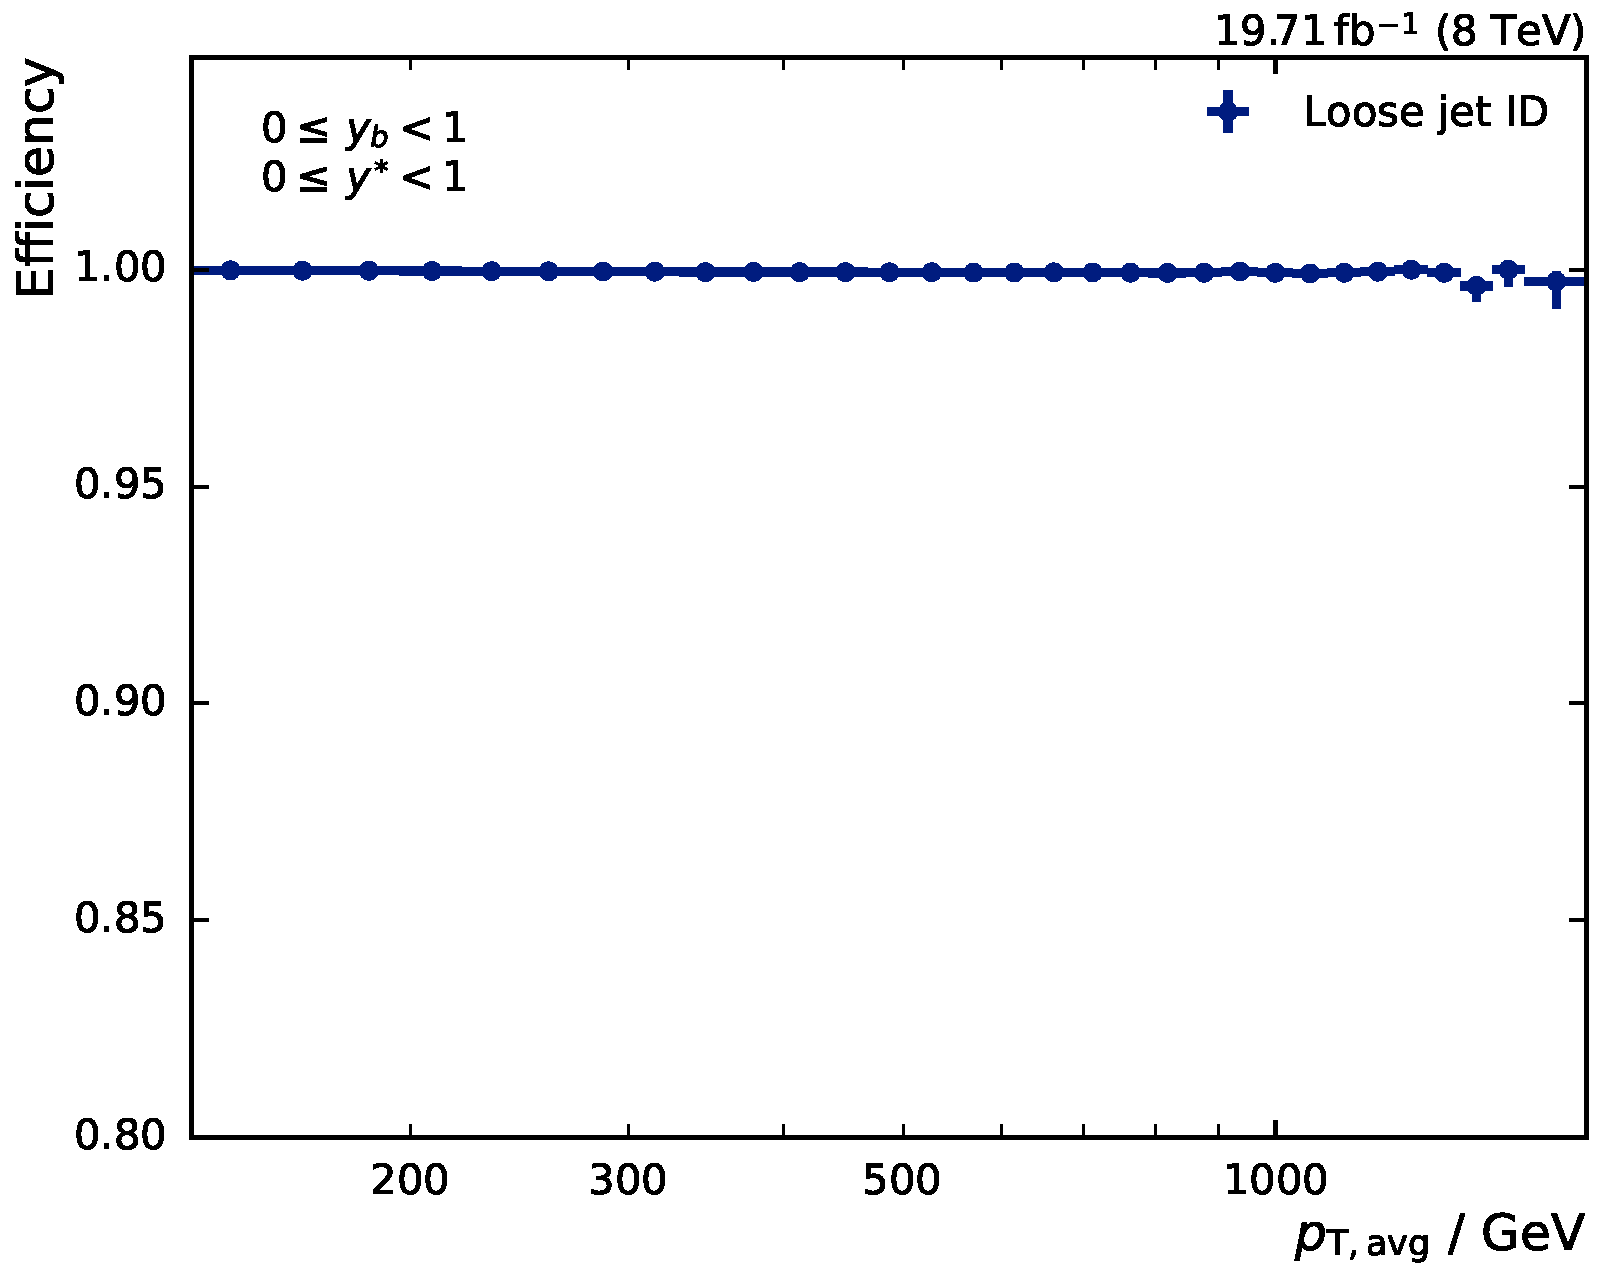
\includegraphics[width=0.45\textwidth]{figures/measurement/jetideff_yb0ys0.pdf}\hfill
    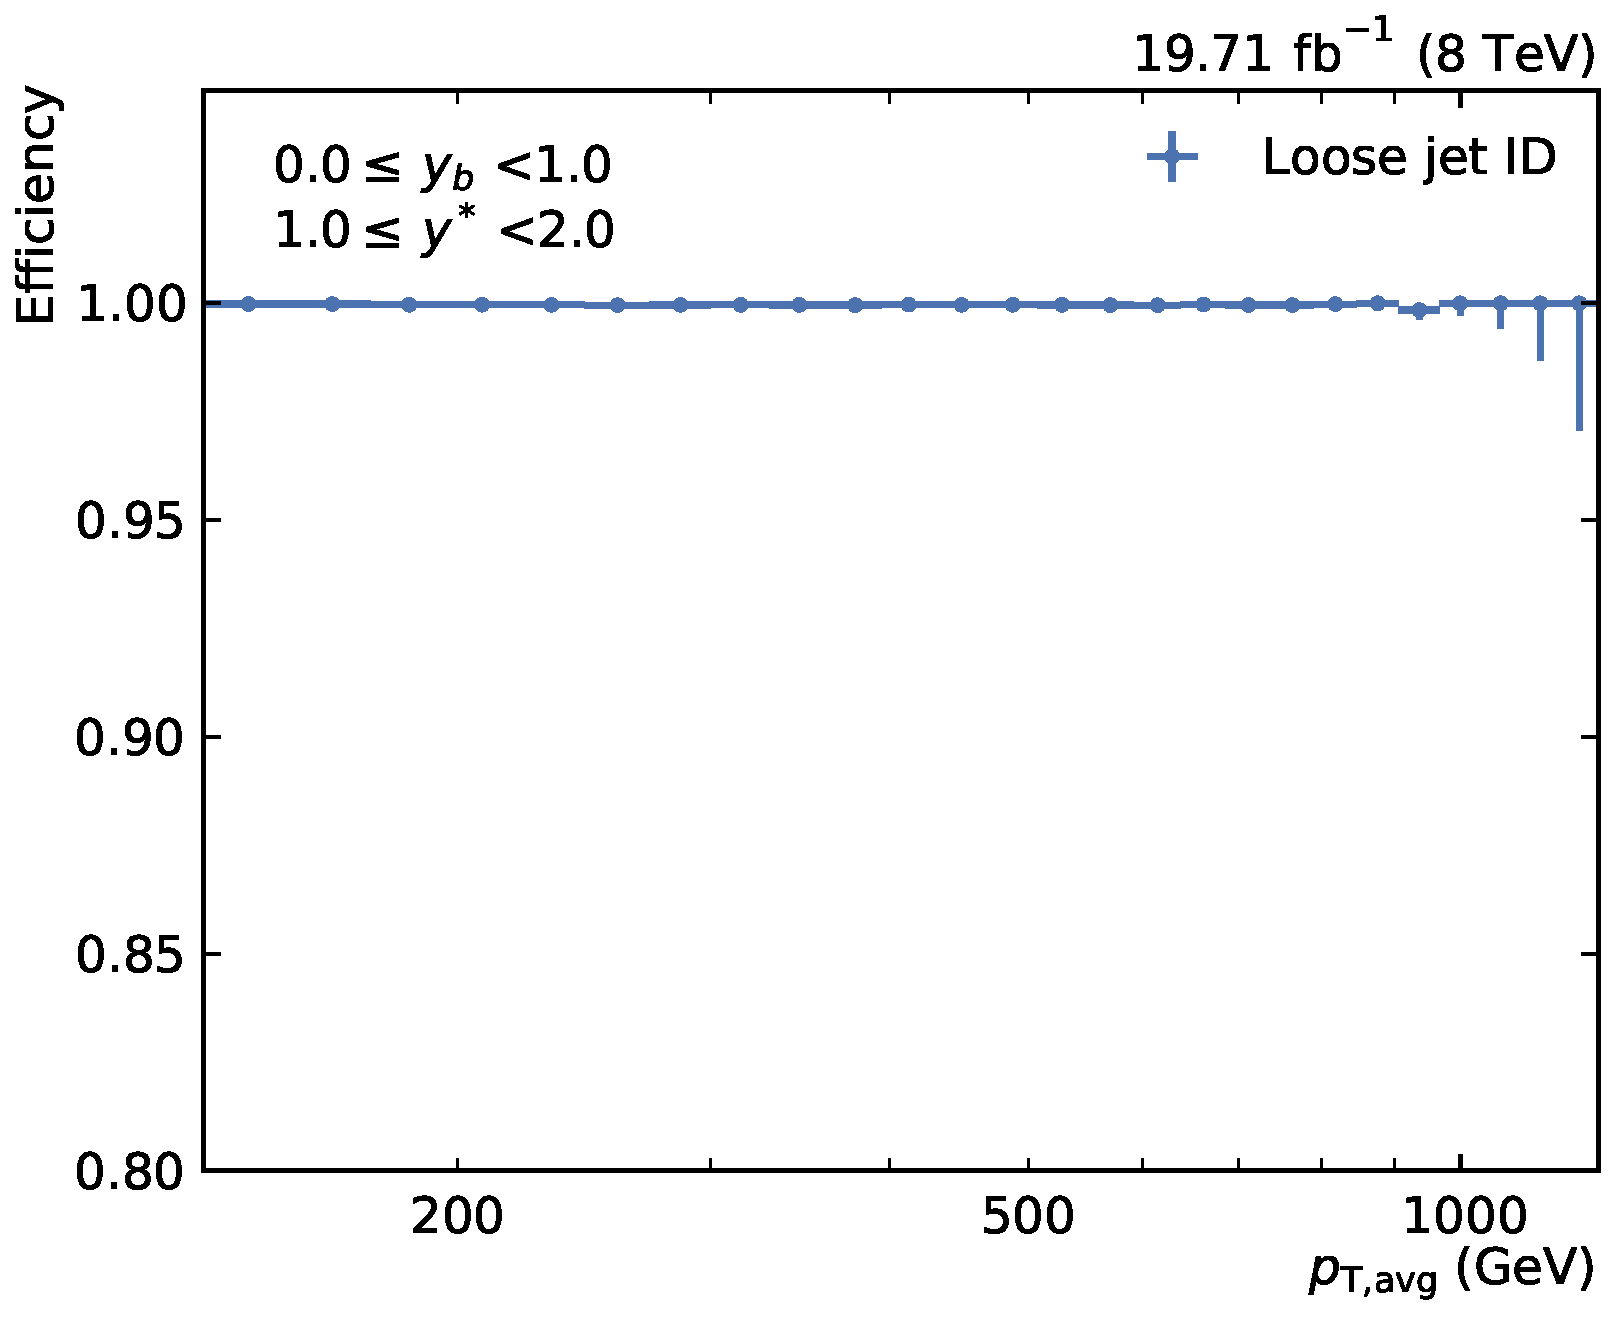
\includegraphics[width=0.45\textwidth]{figures/measurement/jetideff_yb0ys1.pdf}
    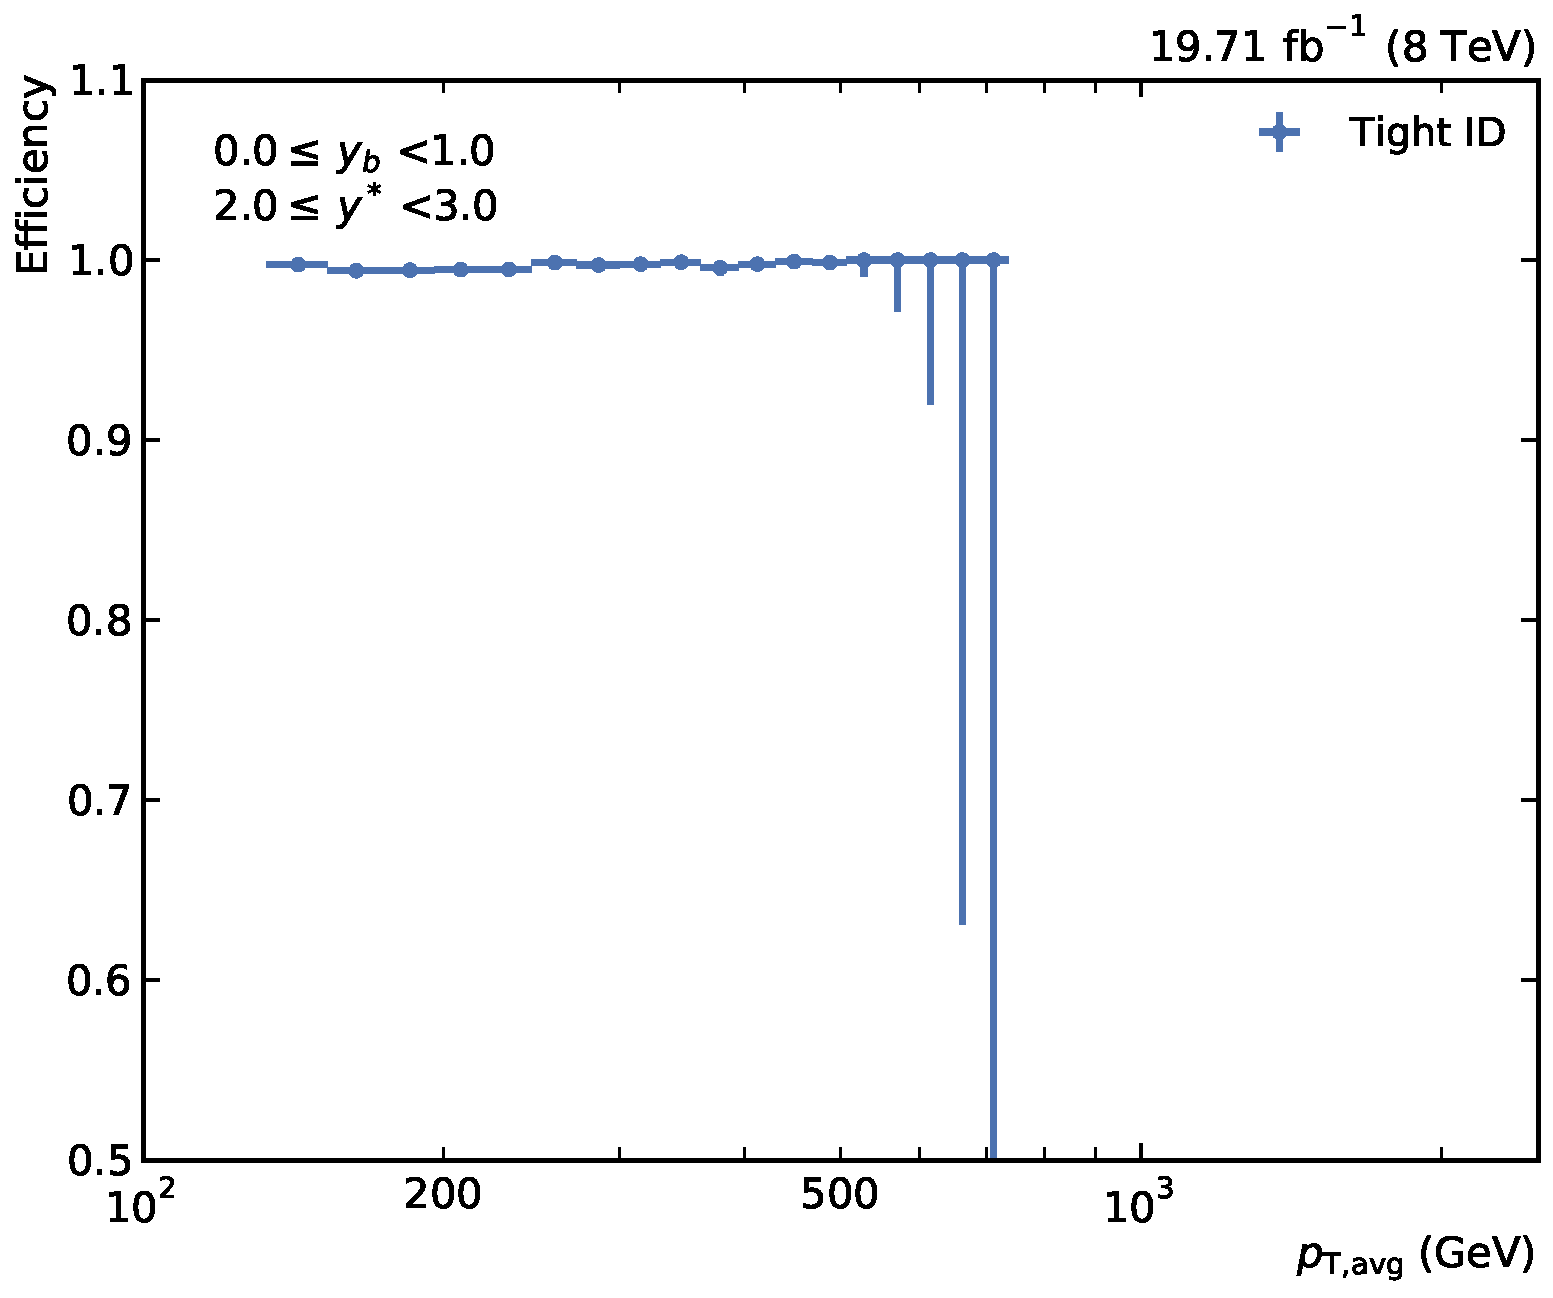
\includegraphics[width=0.45\textwidth]{figures/measurement/jetideff_yb0ys2.pdf}\hfill
    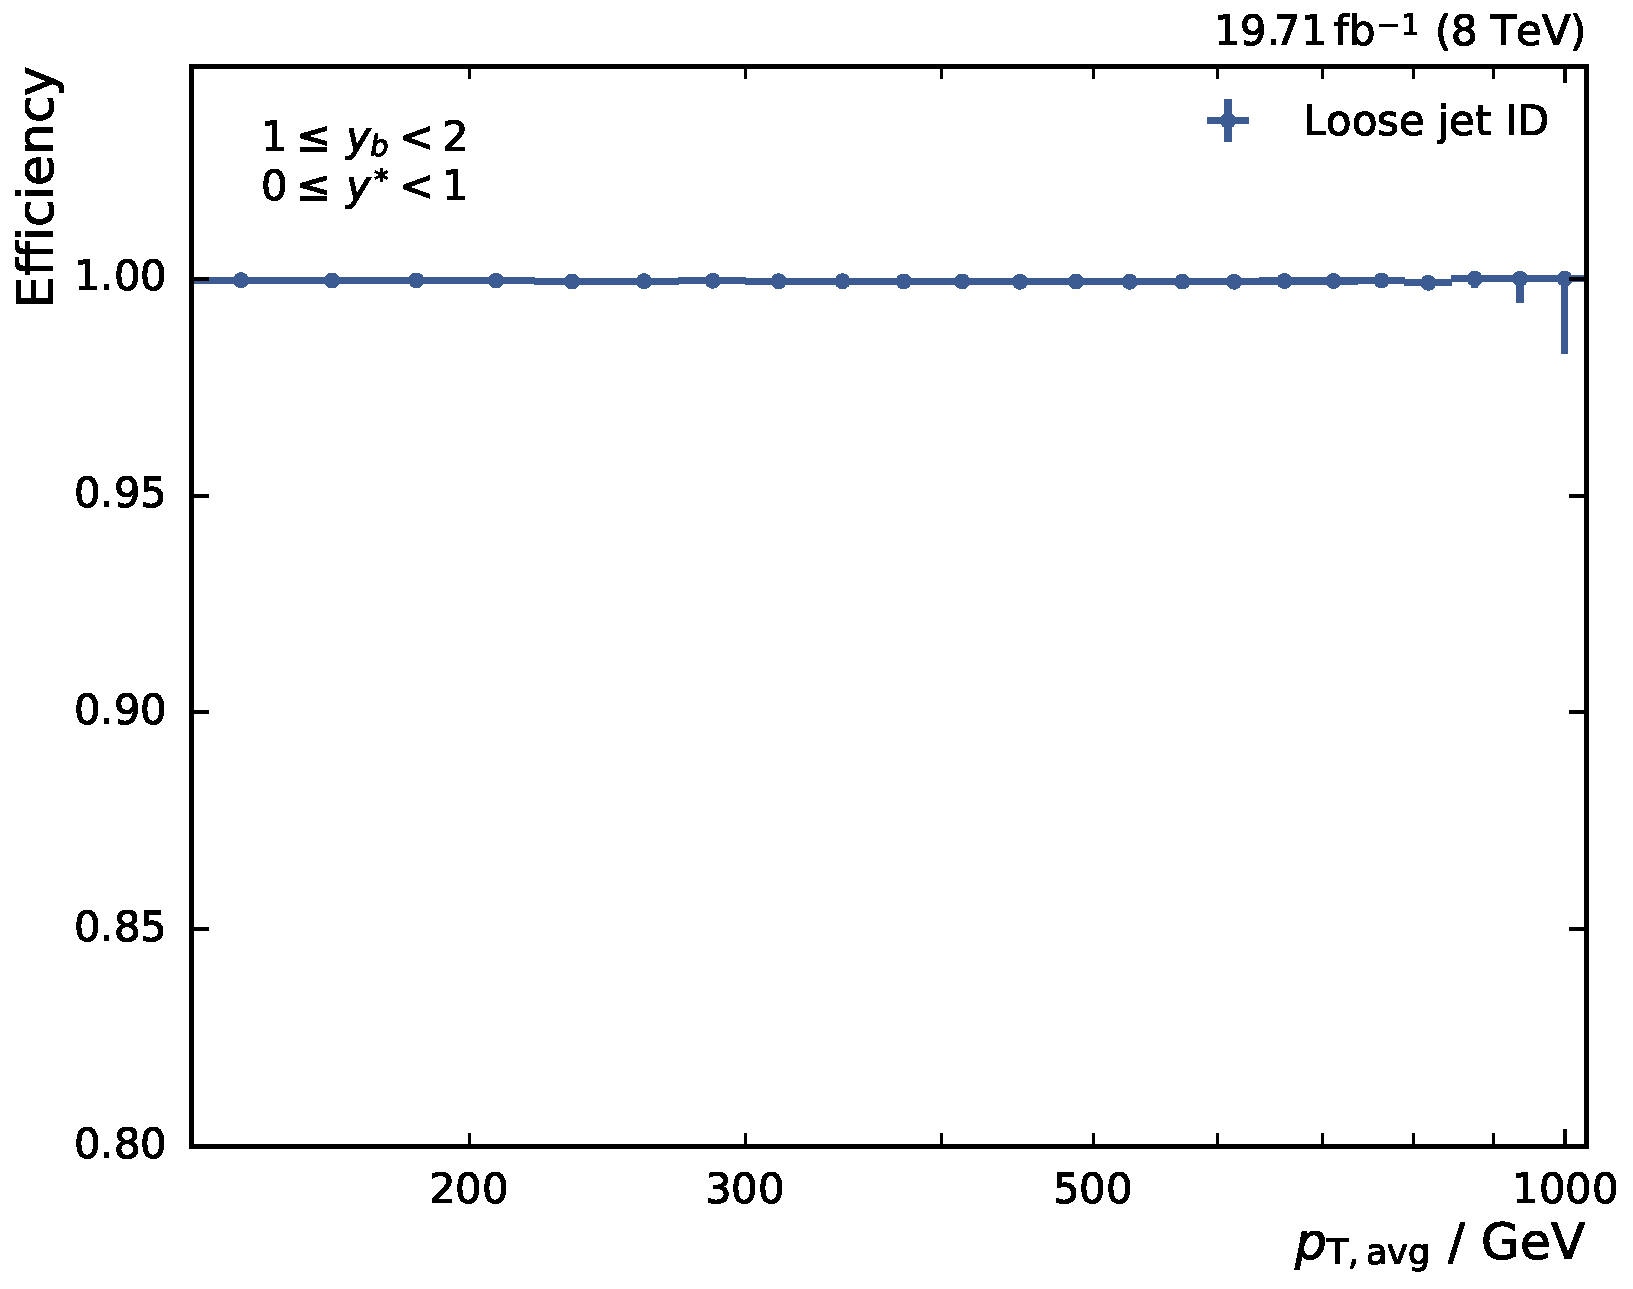
\includegraphics[width=0.45\textwidth]{figures/measurement/jetideff_yb1ys0.pdf}
    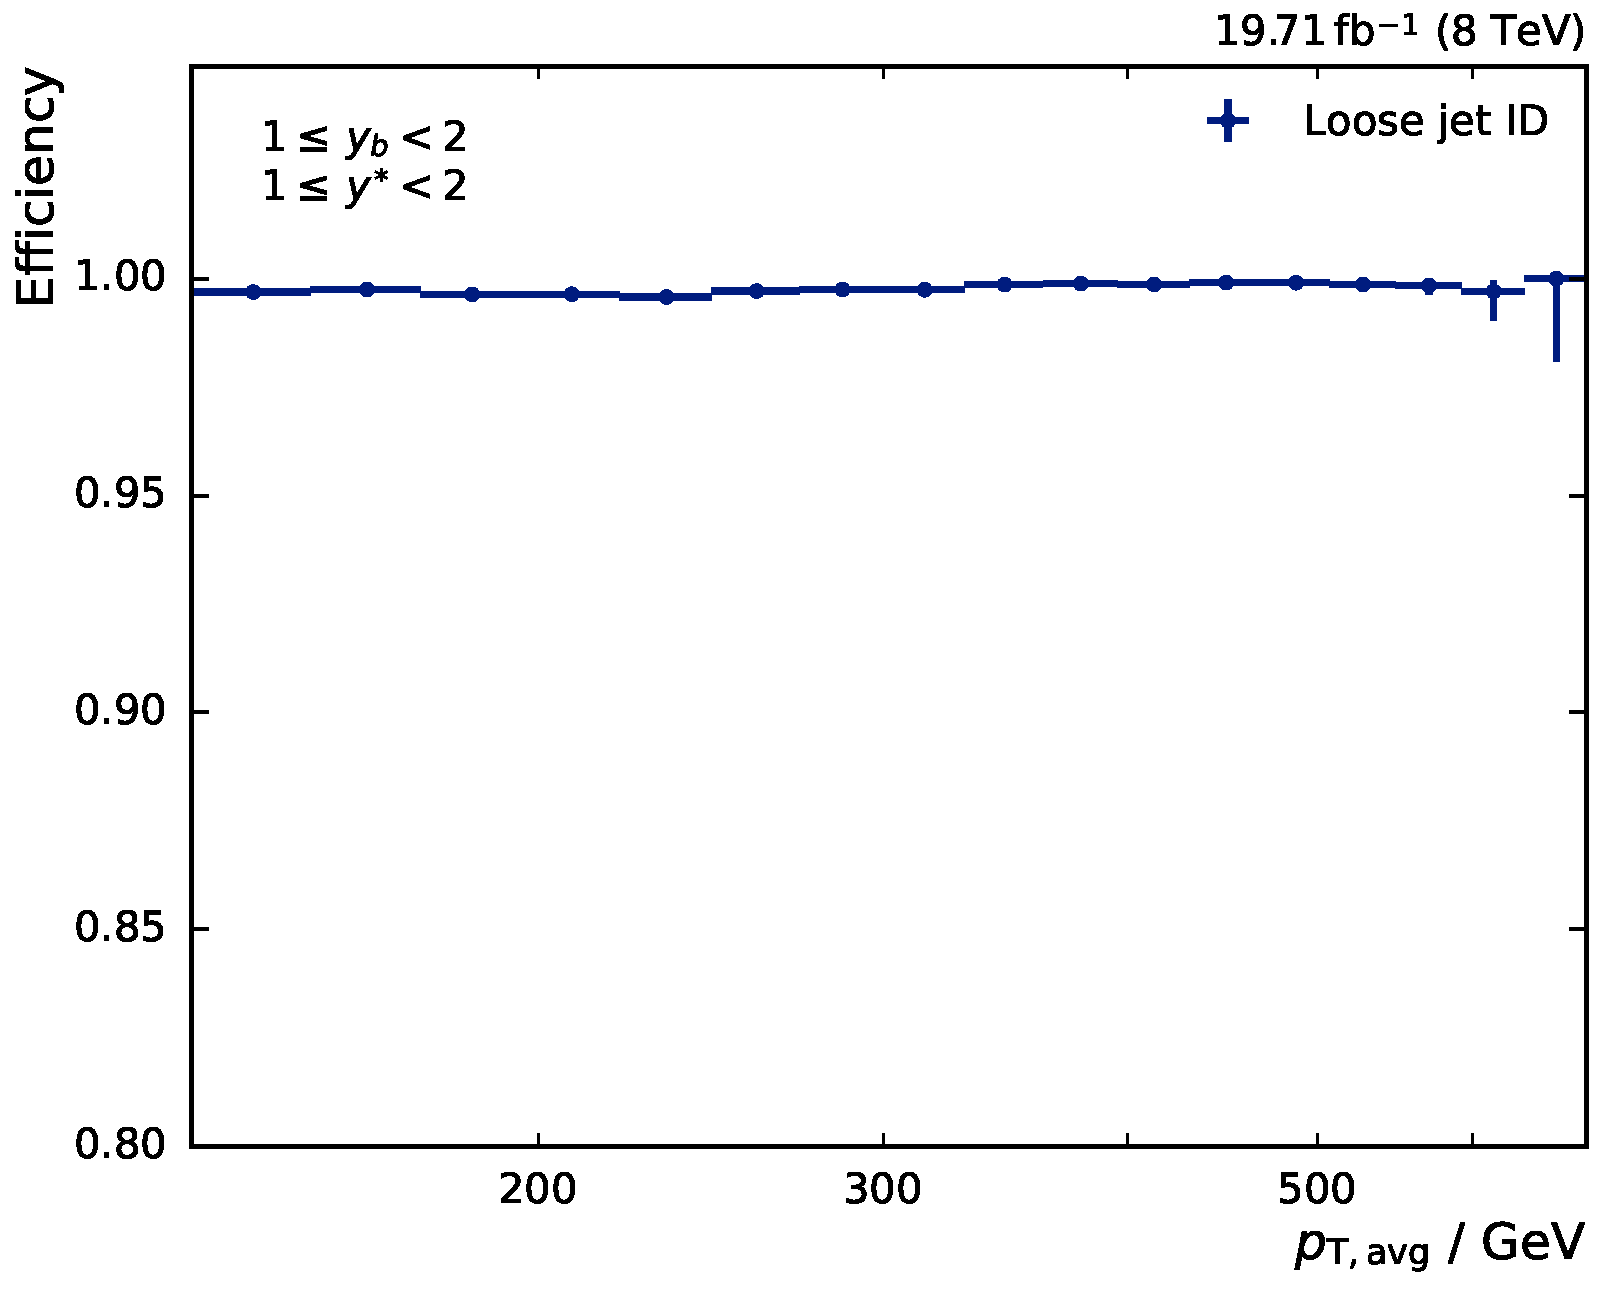
\includegraphics[width=0.45\textwidth]{figures/measurement/jetideff_yb1ys1.pdf}\hfill
    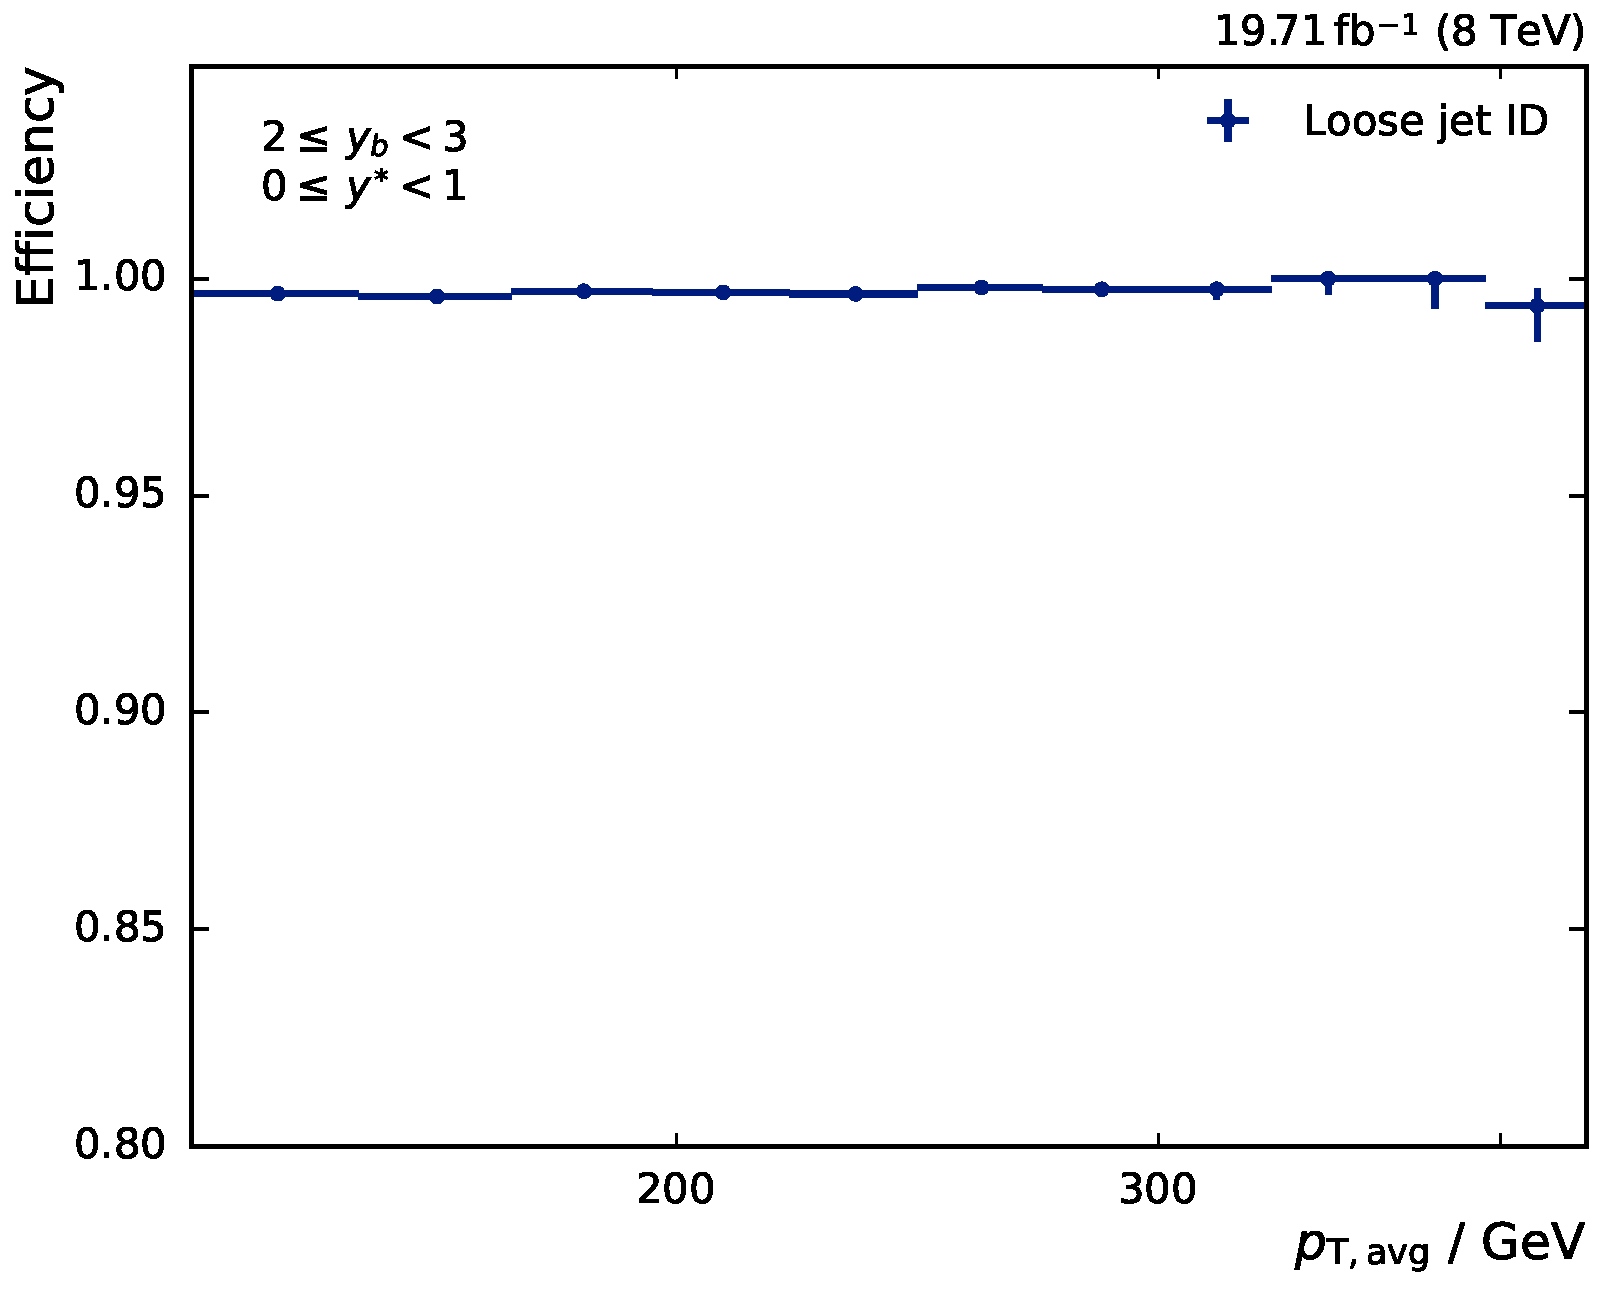
\includegraphics[width=0.45\textwidth]{figures/measurement/jetideff_yb2ys0.pdf}
    \caption[Efficiency of the jet ID]{Jet ID efficiency studied using a
    tag-and-probe approach on clear dijet event signatures. The efficiency is
    shown as a function of the average dijet \pt for all bins in \ystar \yboost. The
    efficiency is in all cases larger than 99\%..}
    \label{fig:jetid_eff}
\end{figure}

\section{Constrol distributions}

Figure~\ref{fig:controlplots:properties} show the numerous energy fractions of the jet constituents. The top
row of this figure show the charged and neutral fraction of hadrons in the jet. The middle row shows
the fraction of muons and photons within the jet while the bottom row show the electron fraction and
the HF hadron fraction.

\begin{figure}[htbp]
    \centering
    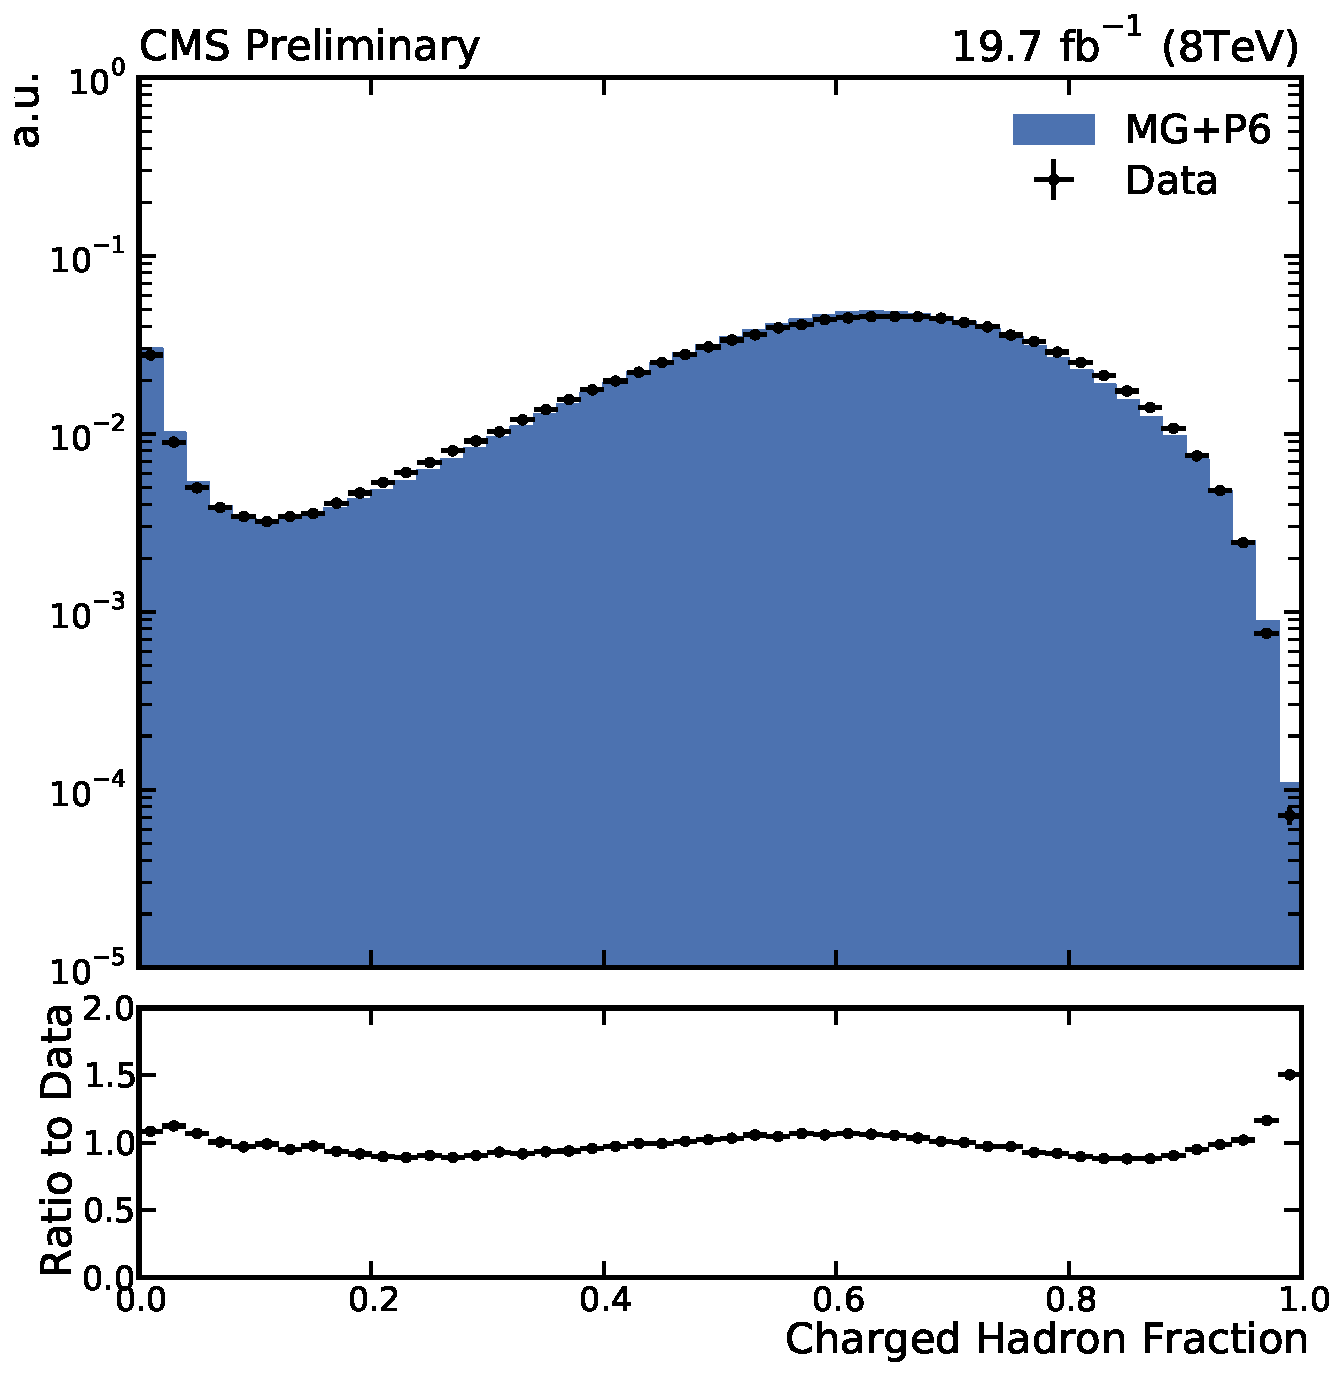
\includegraphics[width=0.45\textwidth]{figures/measurement/jetprop_chf_default.pdf}\hfill
    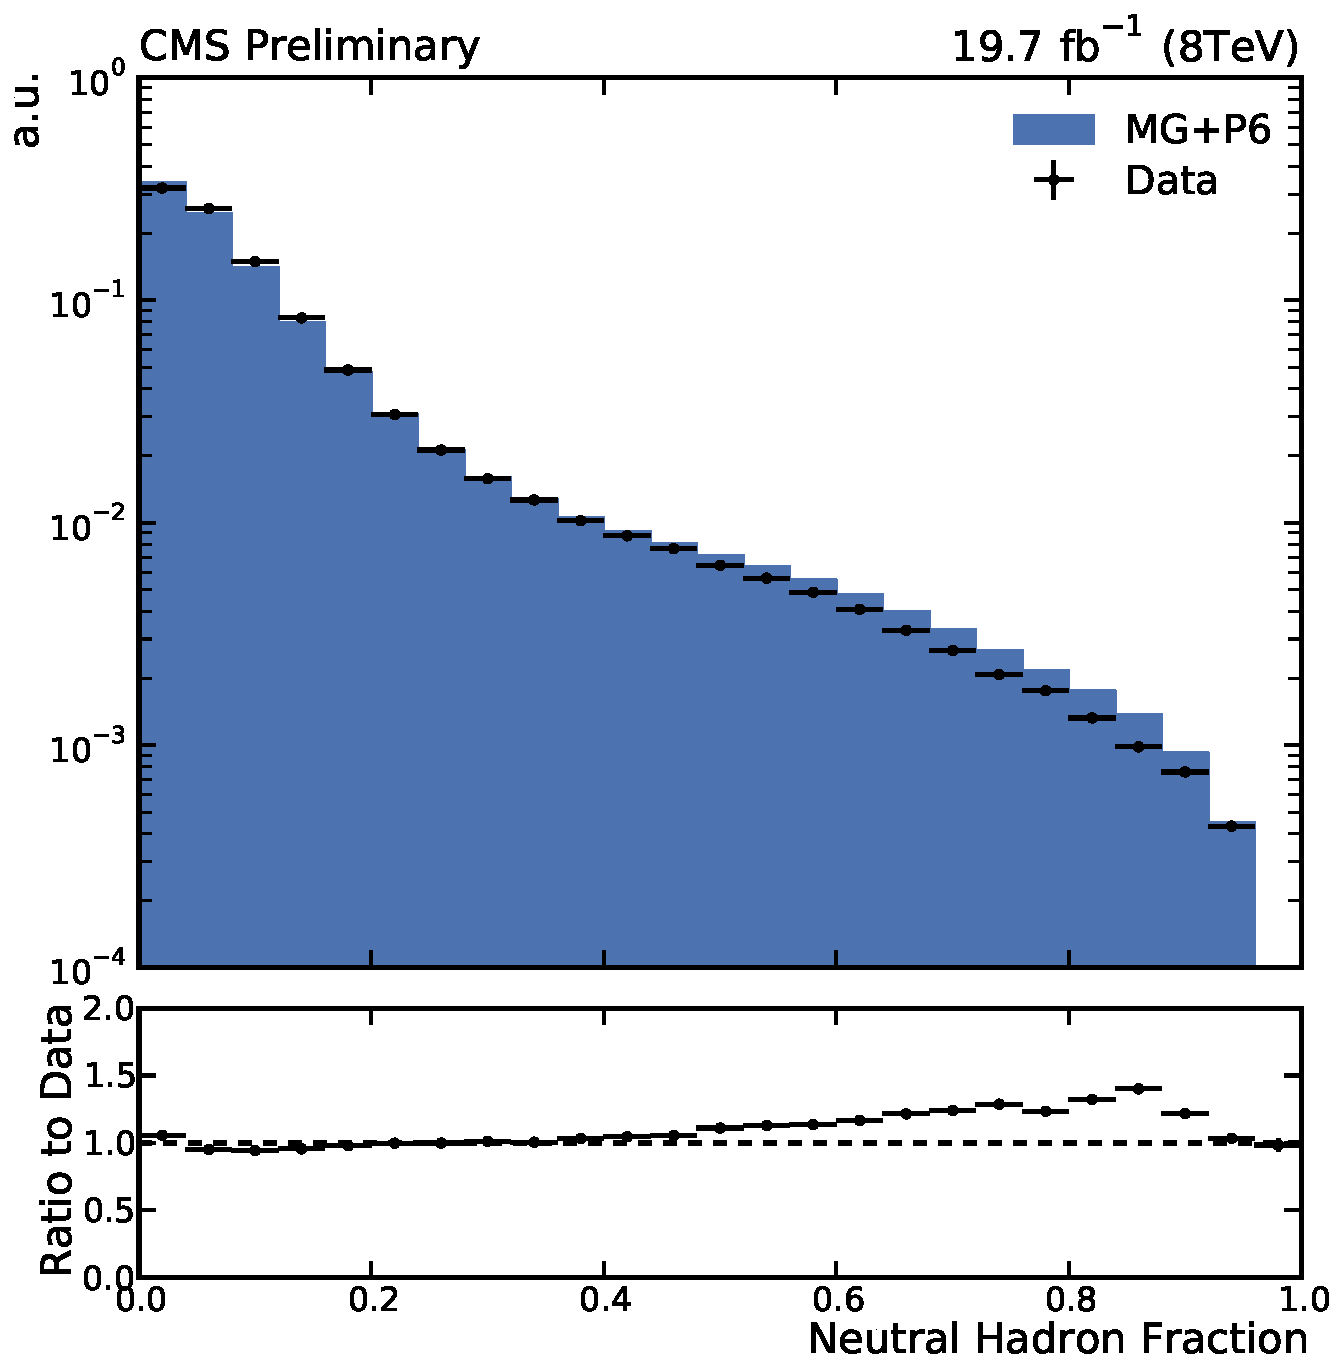
\includegraphics[width=0.45\textwidth]{figures/measurement/jetprop_nhf_default.pdf}
    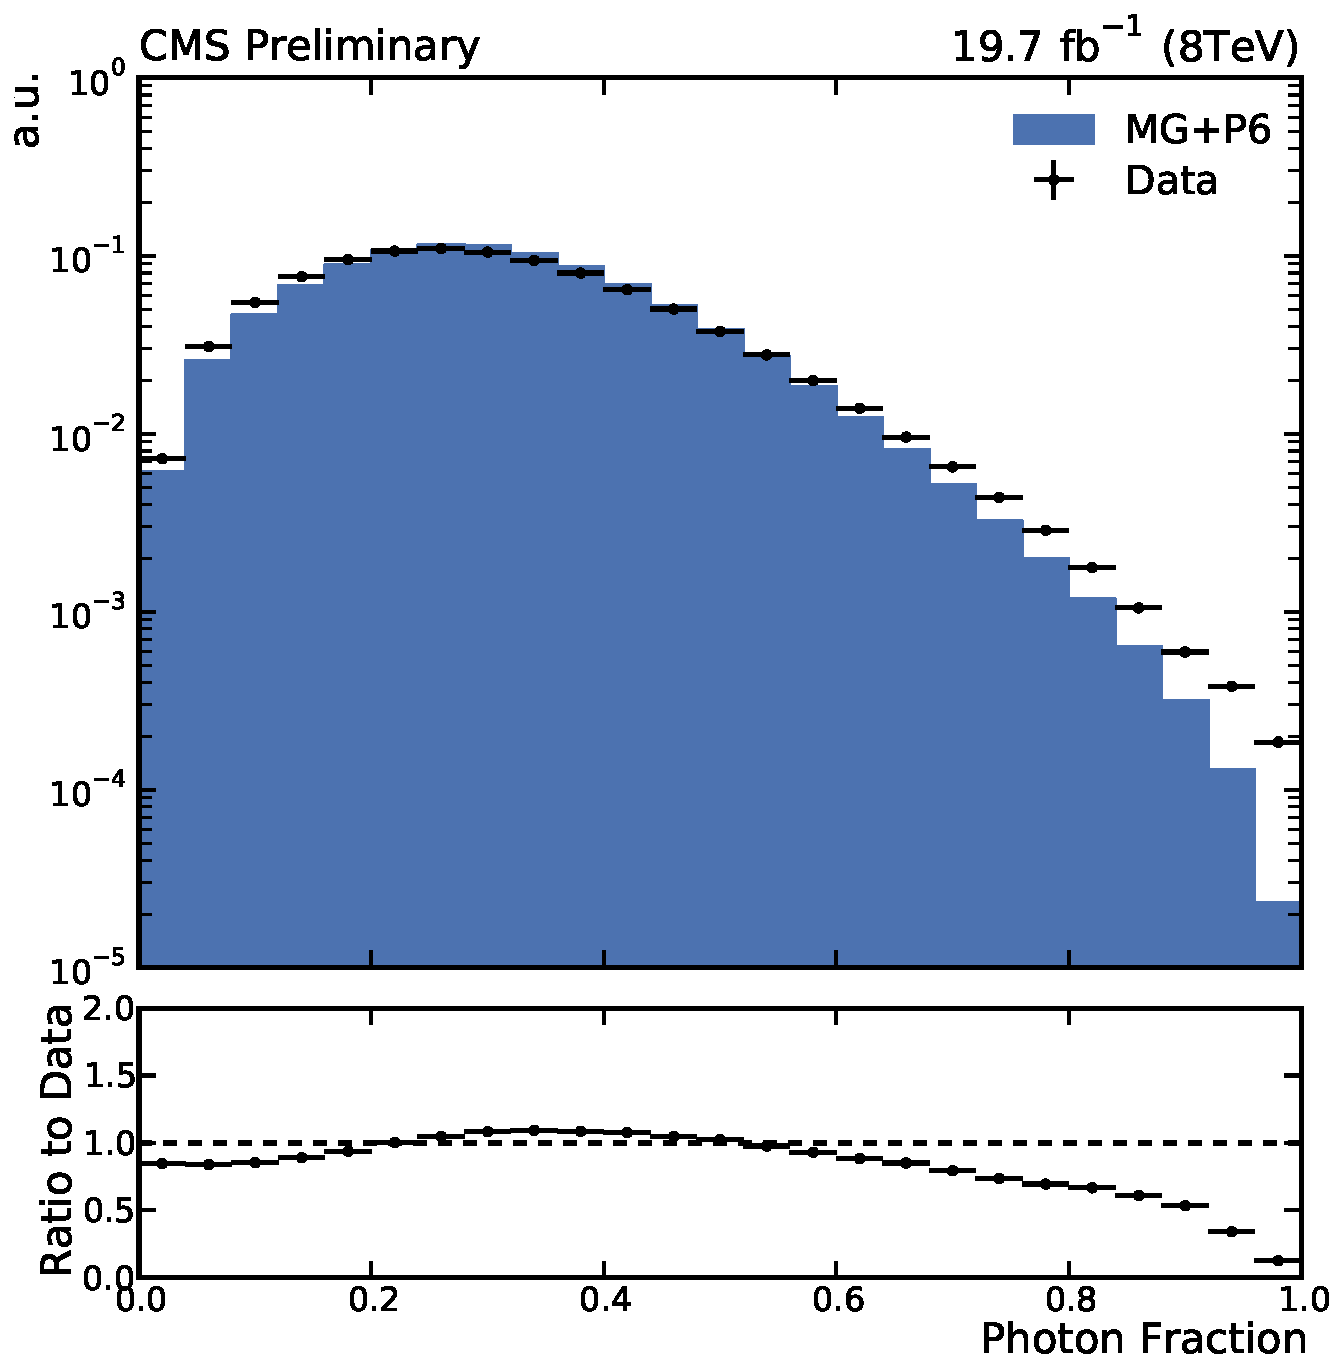
\includegraphics[width=0.45\textwidth]{figures/measurement/jetprop_gammaf_default.pdf}\hfill
    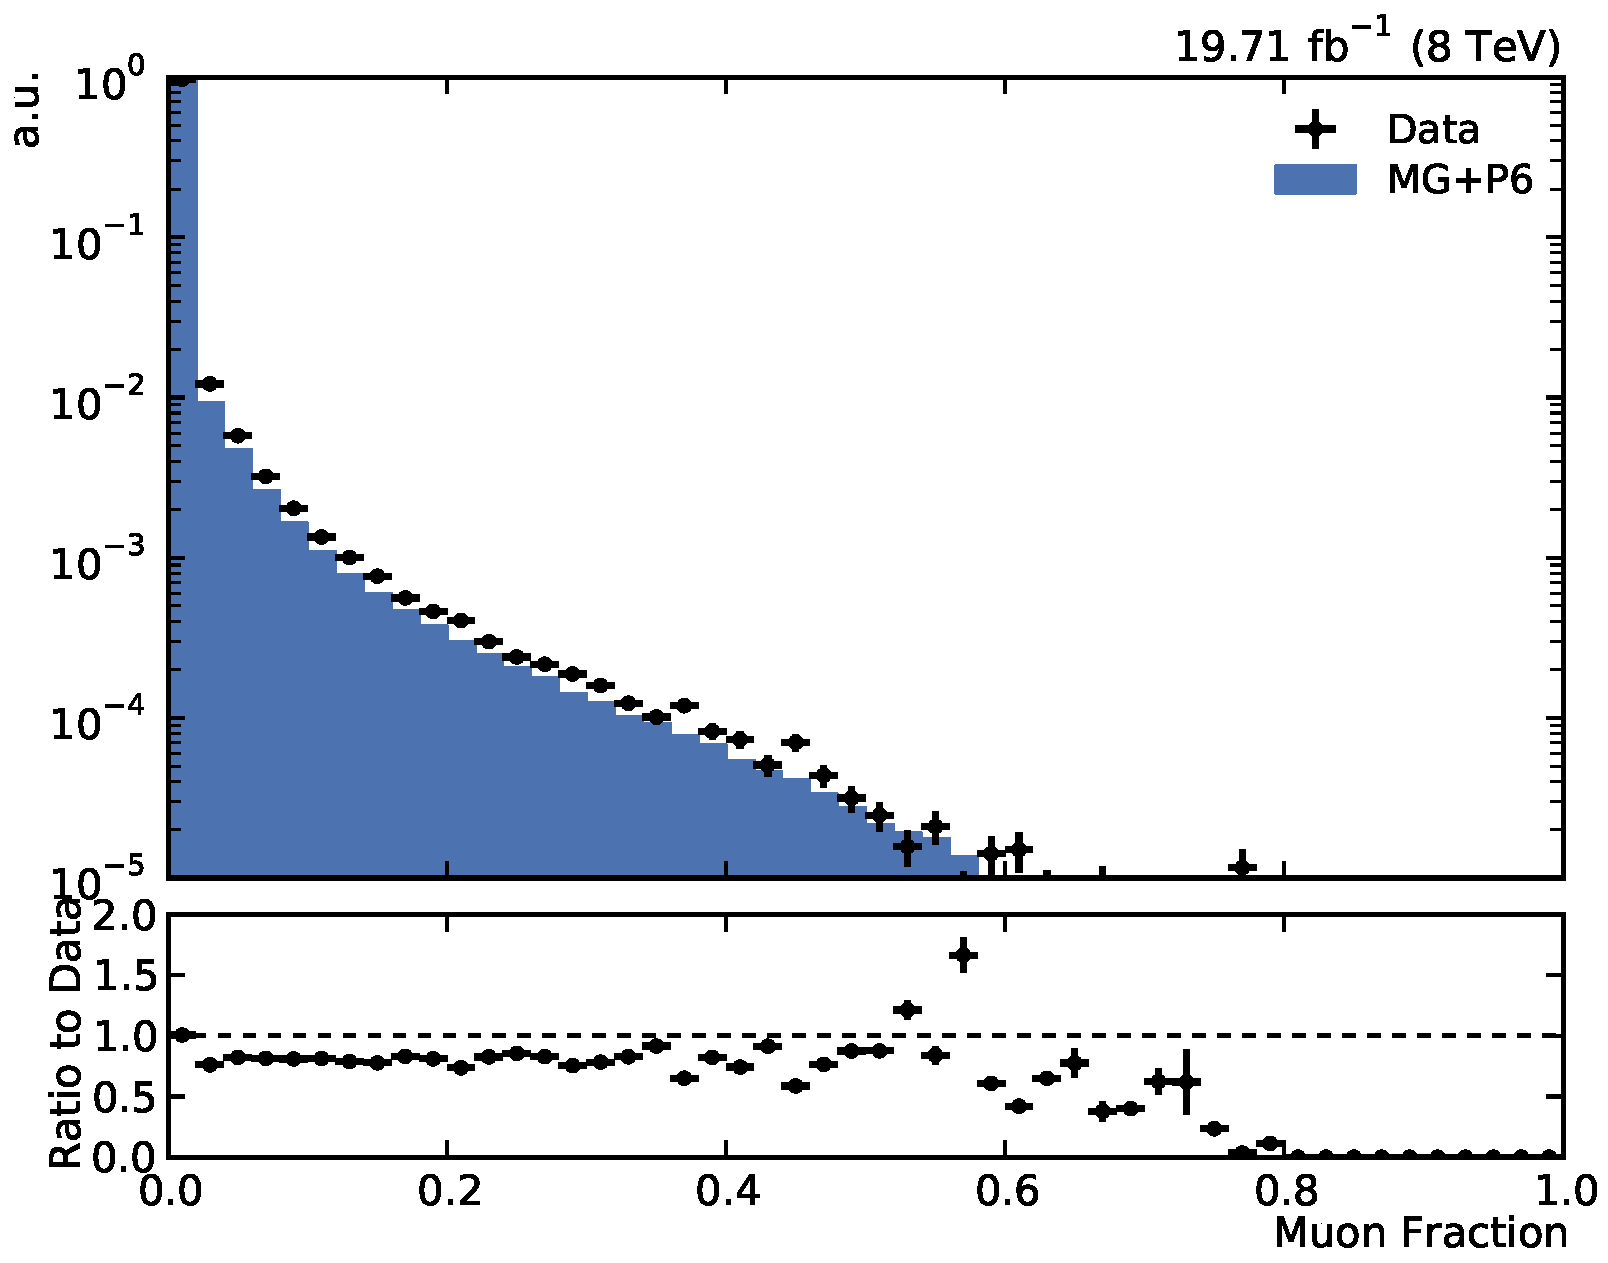
\includegraphics[width=0.45\textwidth]{figures/measurement/jetprop_muf_default.pdf}
    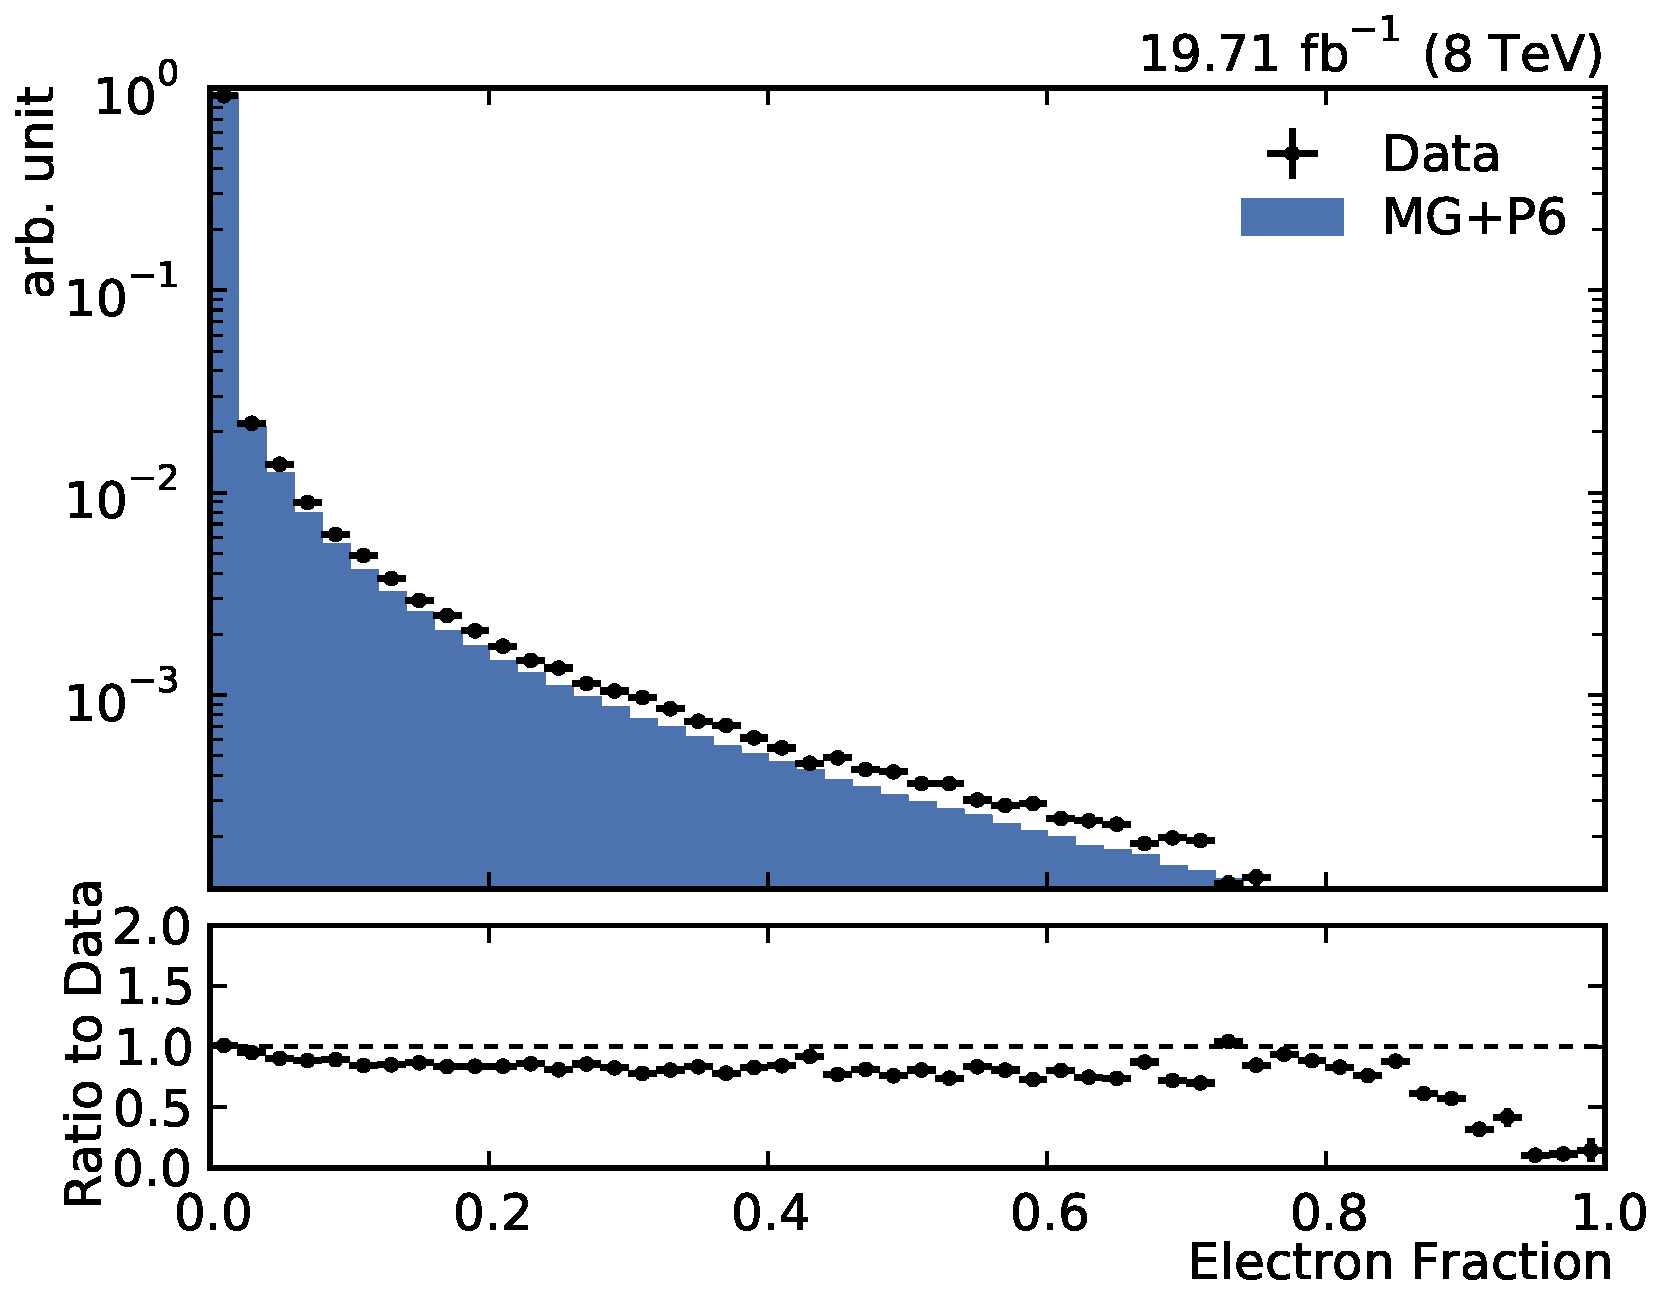
\includegraphics[width=0.45\textwidth]{figures/measurement/jetprop_ef_default.pdf}\hfill
    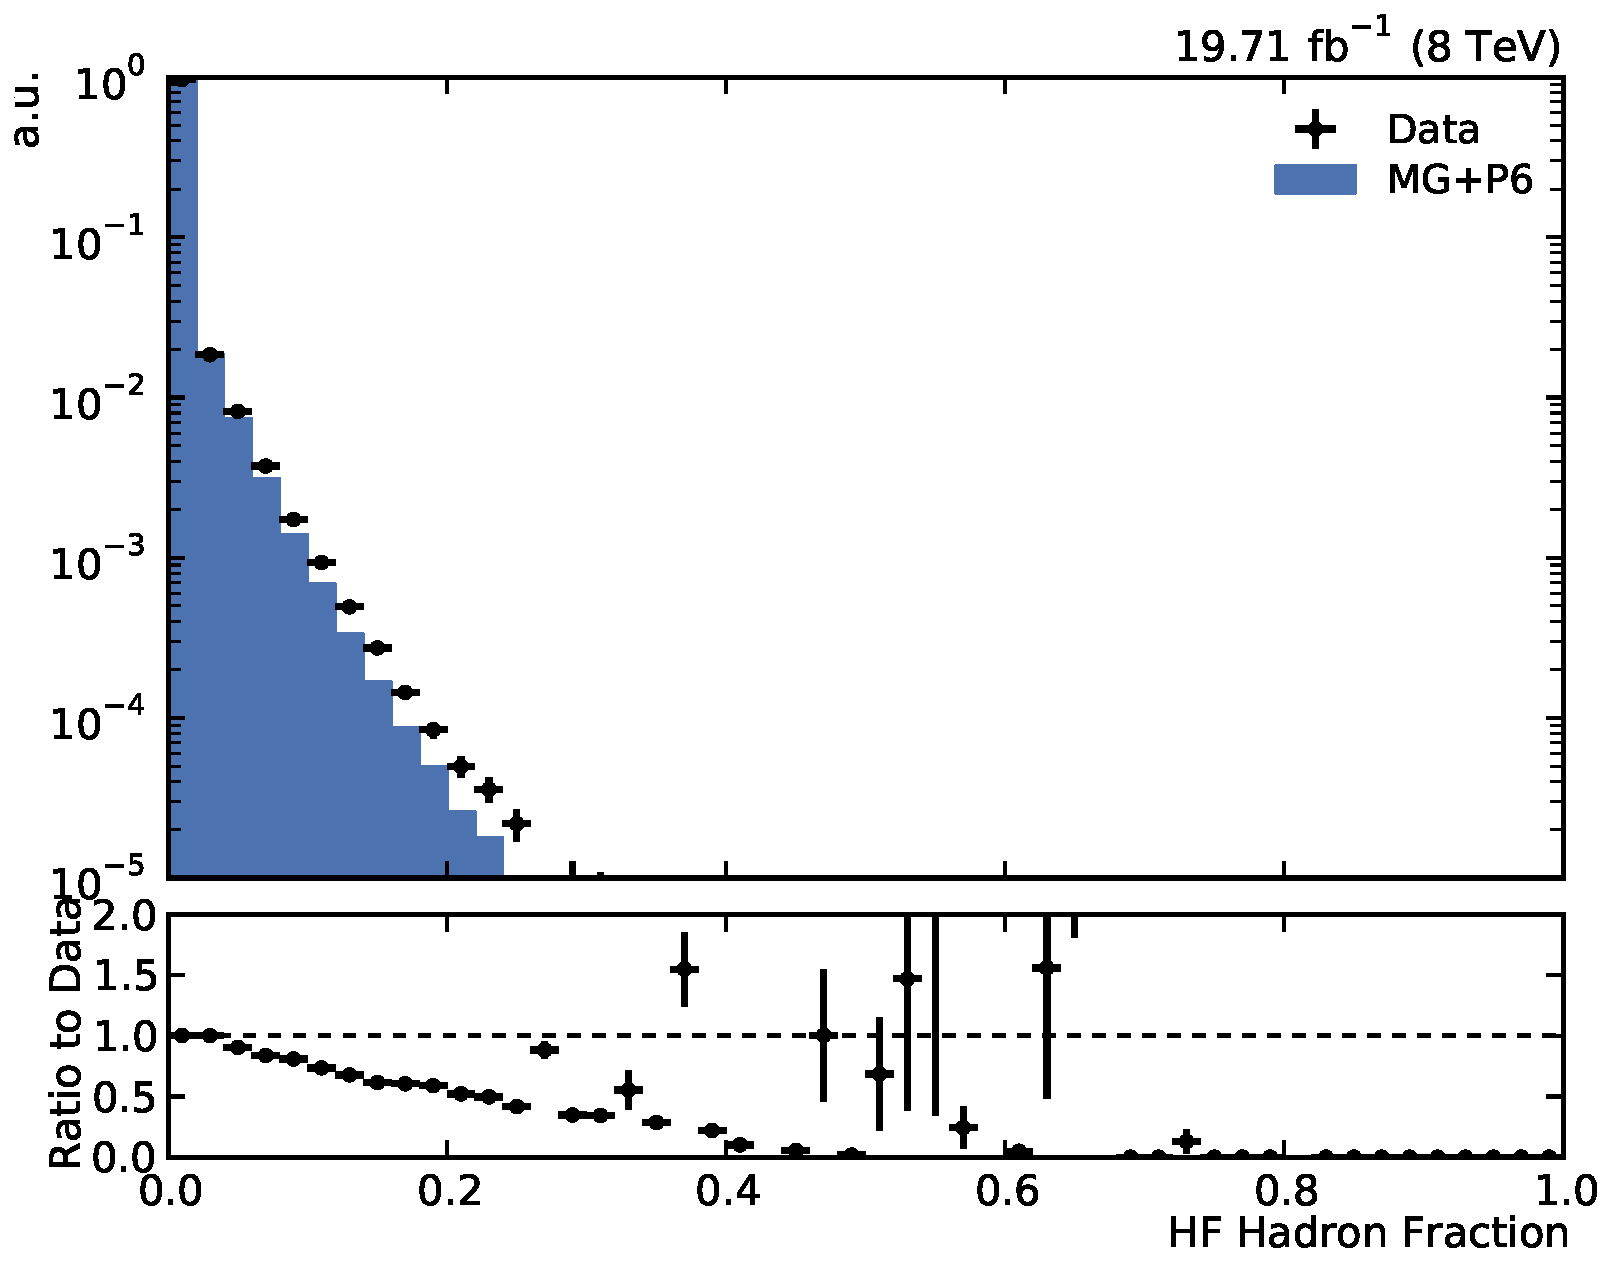
\includegraphics[width=0.45\textwidth]{figures/measurement/jetprop_hf_emf_default.pdf}
    \caption{Control distribution for the jet constituent fractions. .}
    \label{fig:controlplots:properties}
\end{figure}


\section{Individual sources of Jet energy correction uncertainties}

The following figures show the individual components of the jet energy correction uncertainties.

\begin{figure}[htbp]
    \centering
    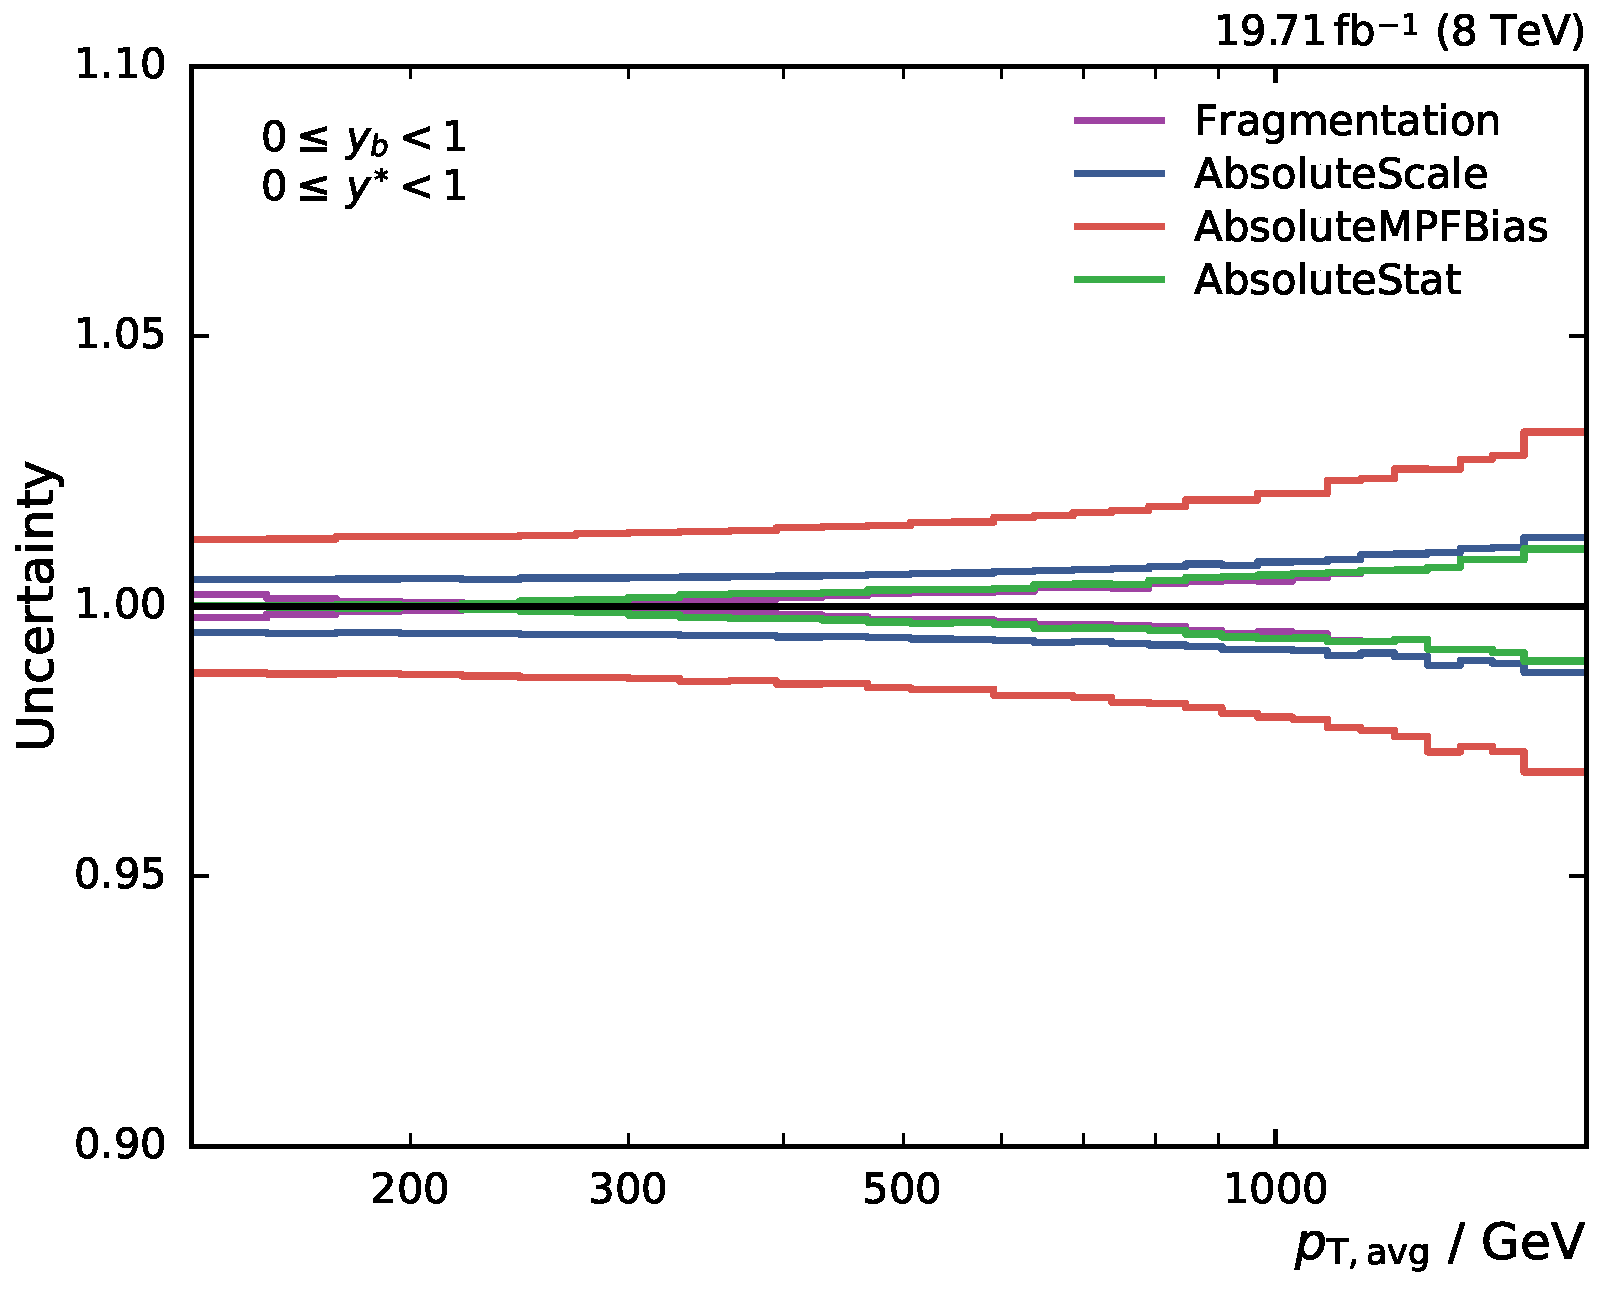
\includegraphics[width=0.45\textwidth]{figures/measurement/jec_relunc_0_yb0ys0.pdf}\hfill
    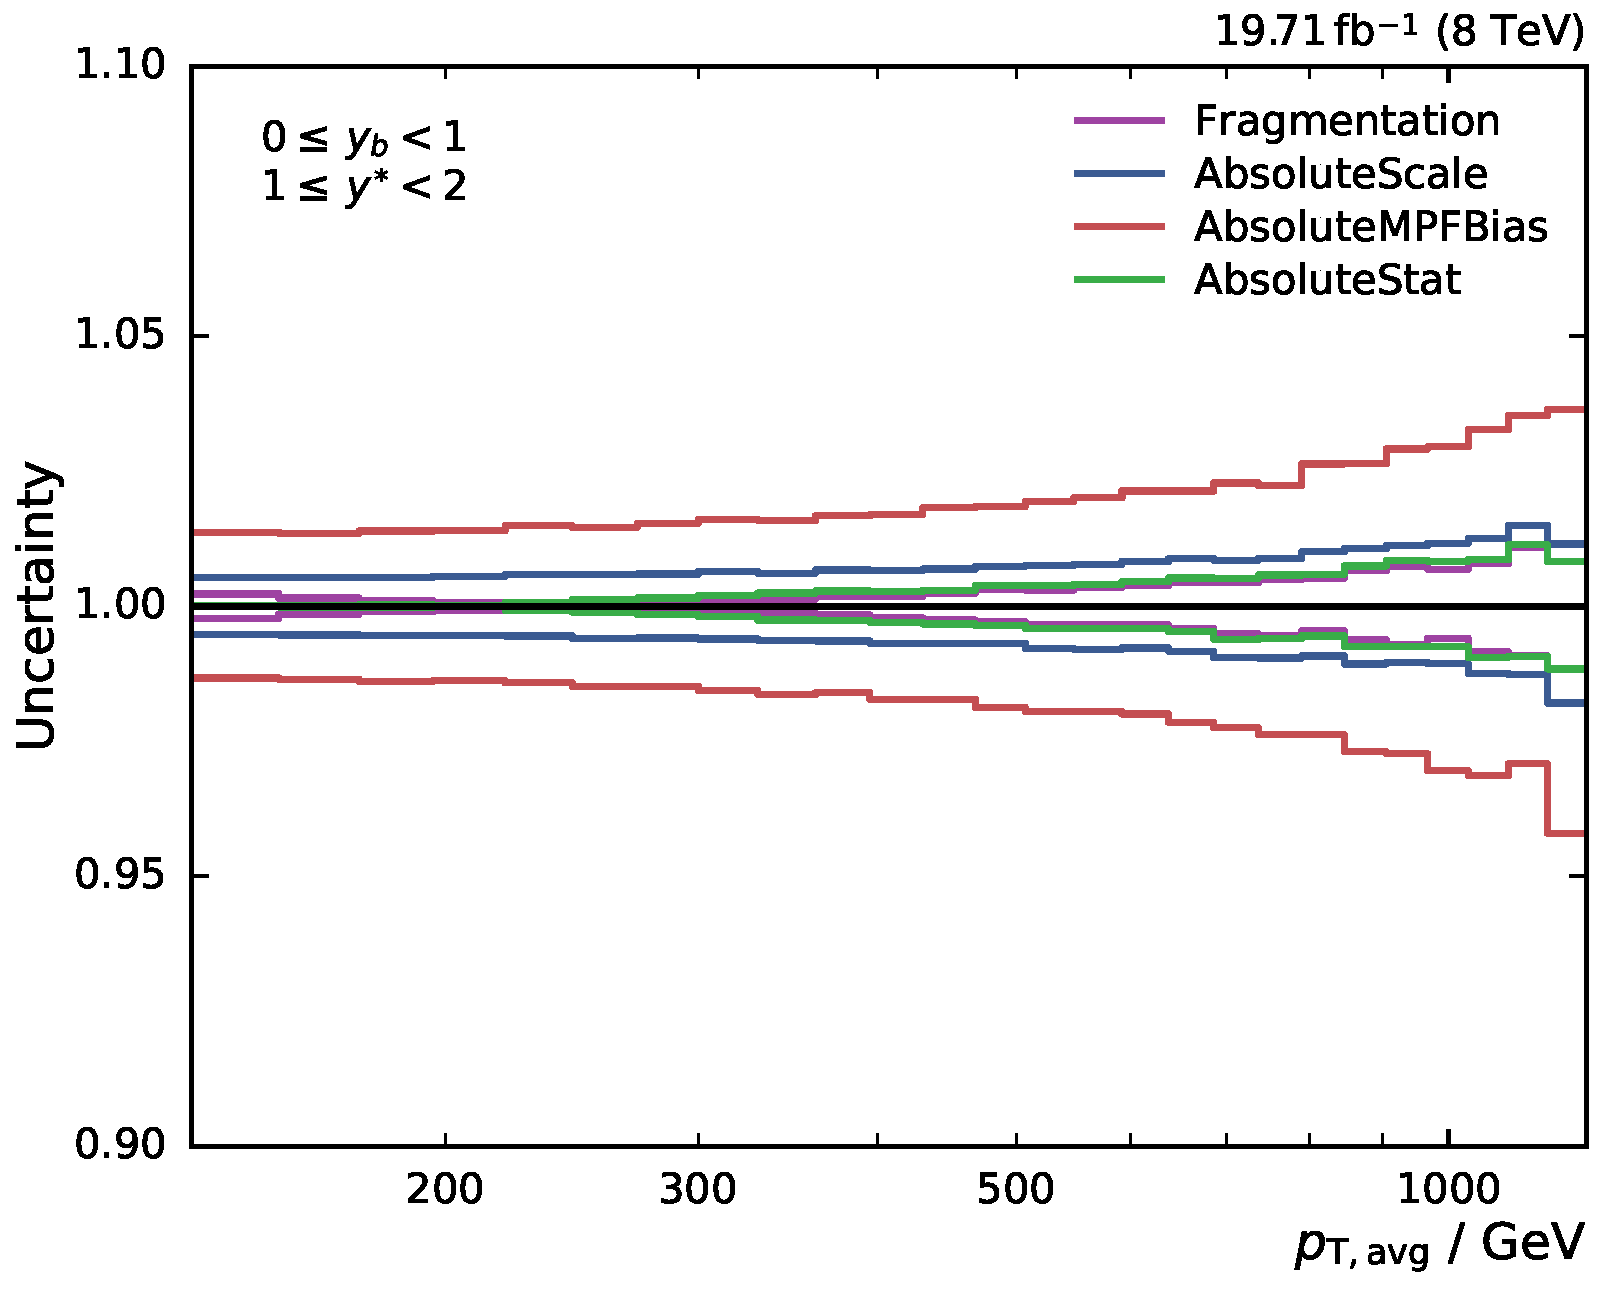
\includegraphics[width=0.45\textwidth]{figures/measurement/jec_relunc_0_yb0ys1.pdf}
    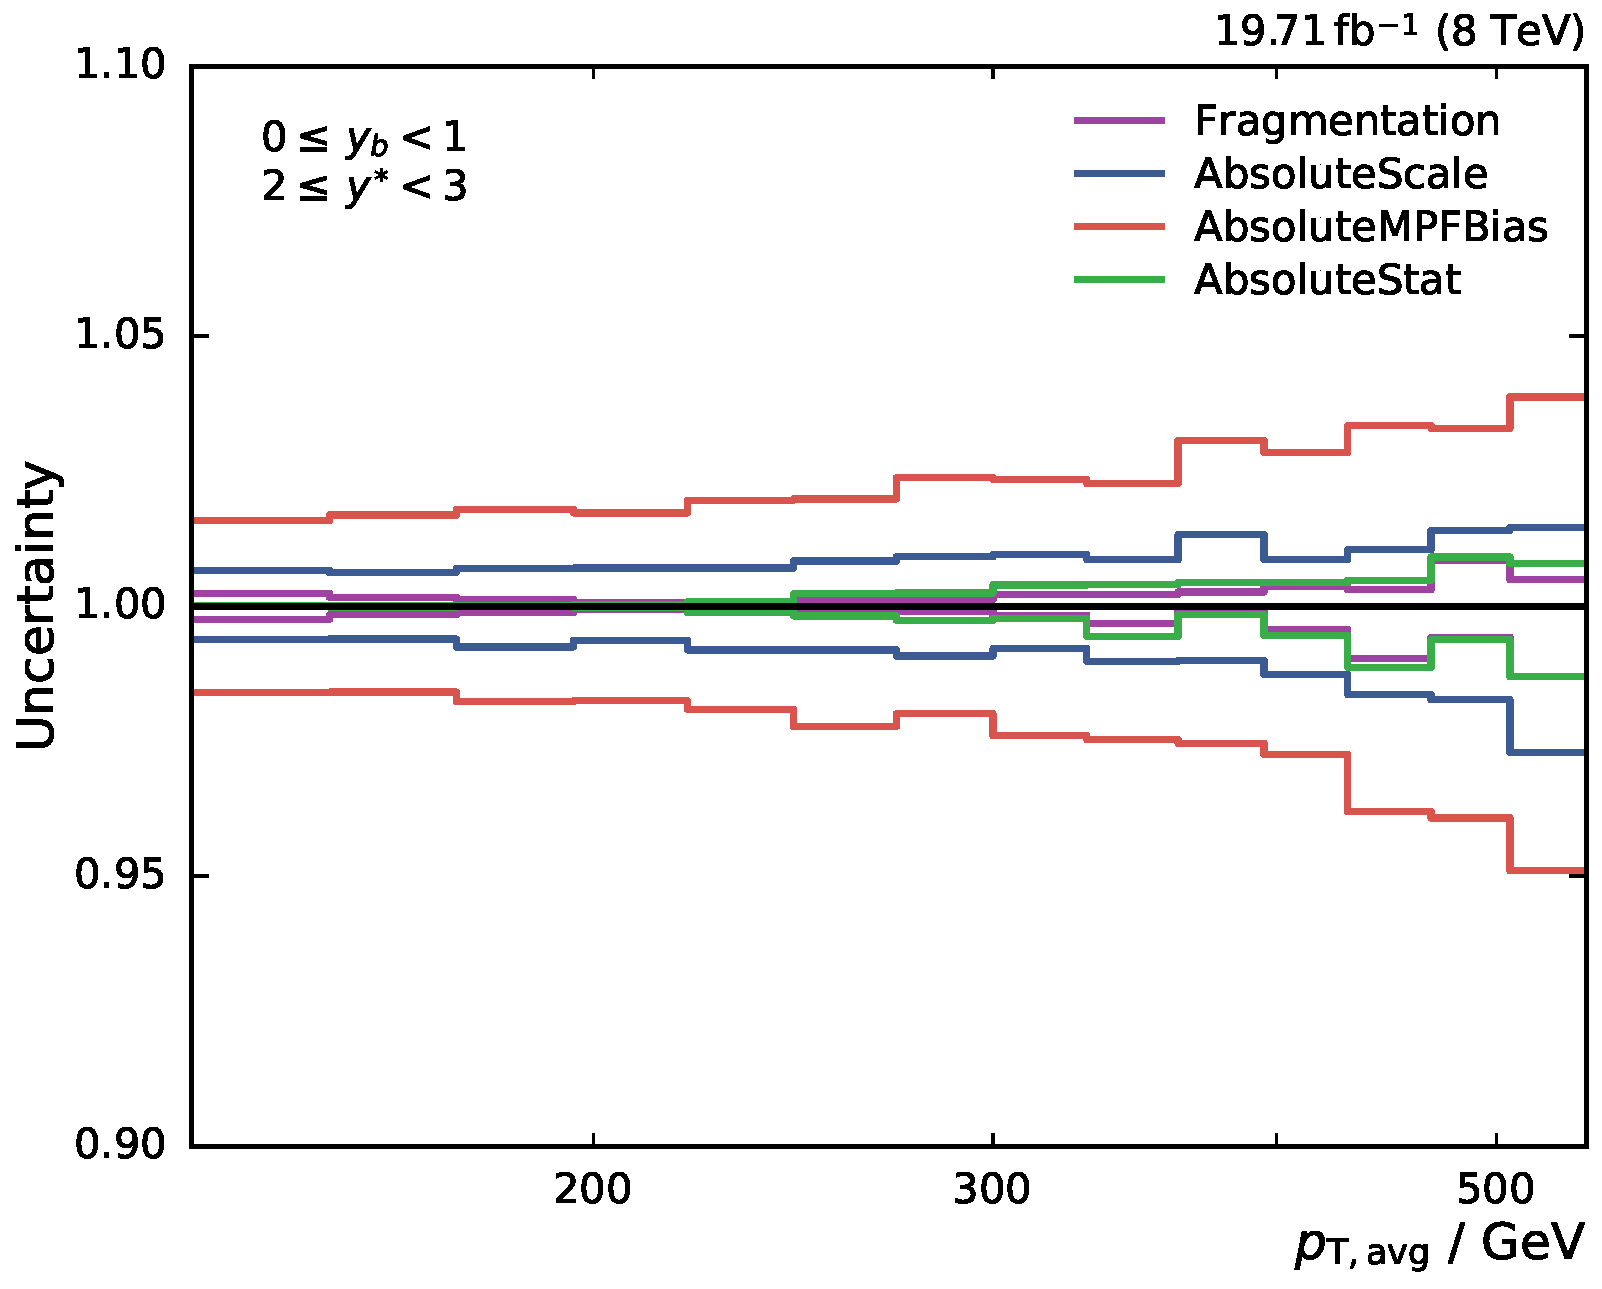
\includegraphics[width=0.45\textwidth]{figures/measurement/jec_relunc_0_yb0ys2.pdf}\hfill
    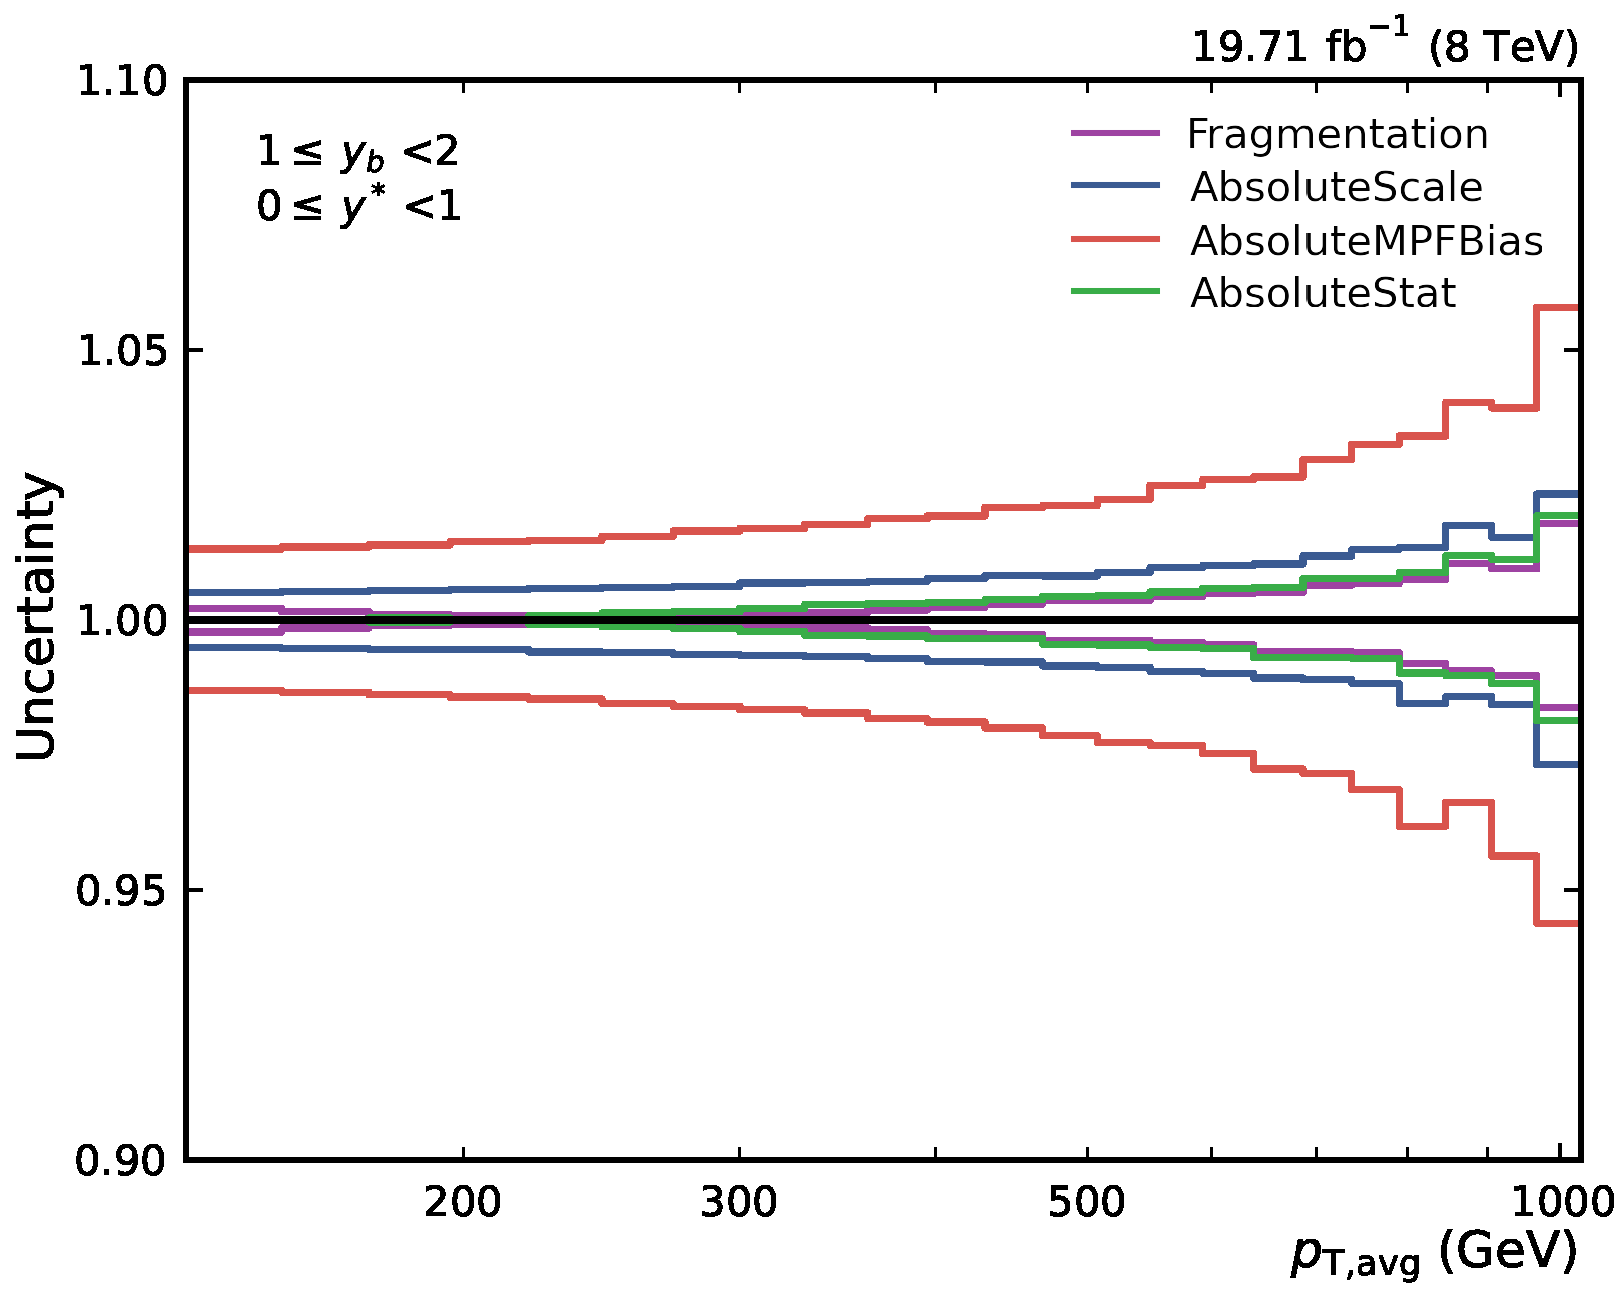
\includegraphics[width=0.45\textwidth]{figures/measurement/jec_relunc_0_yb1ys0.pdf}
    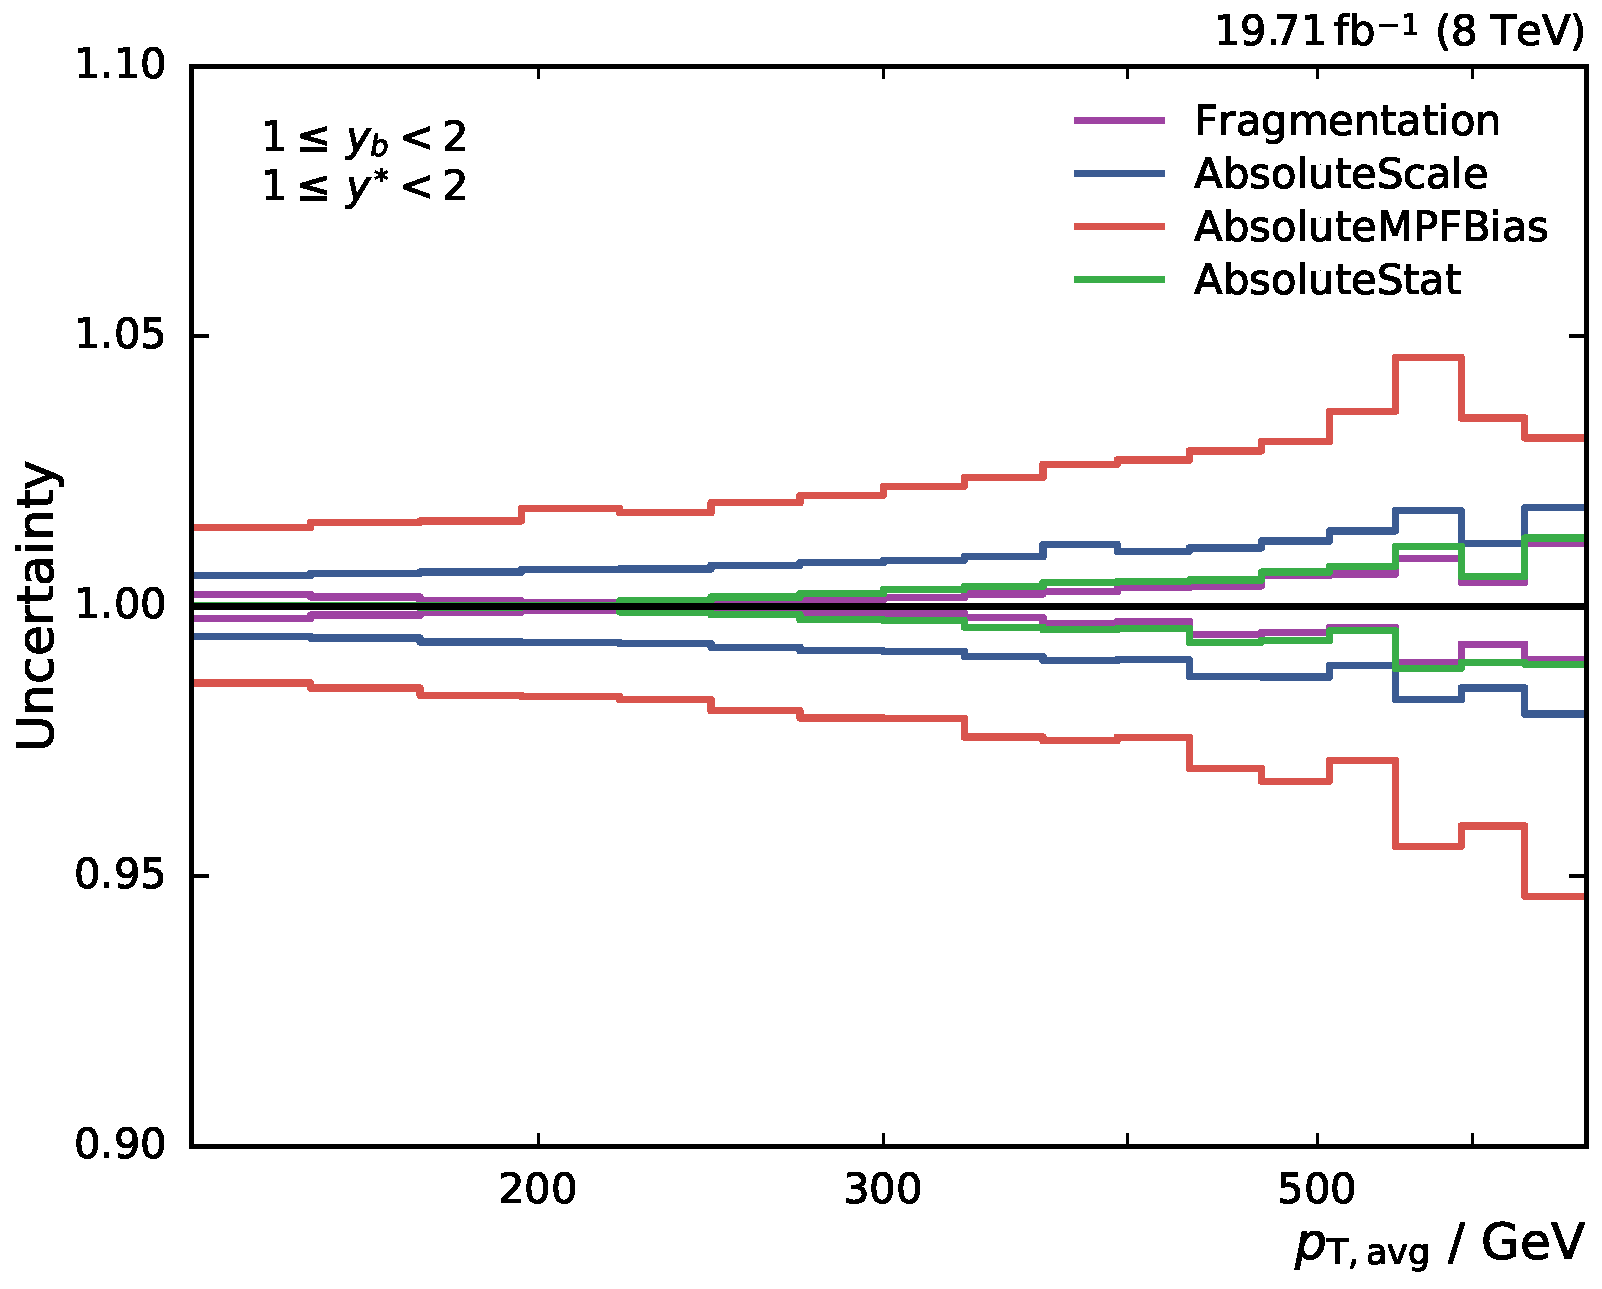
\includegraphics[width=0.45\textwidth]{figures/measurement/jec_relunc_0_yb1ys1.pdf}\hfill
    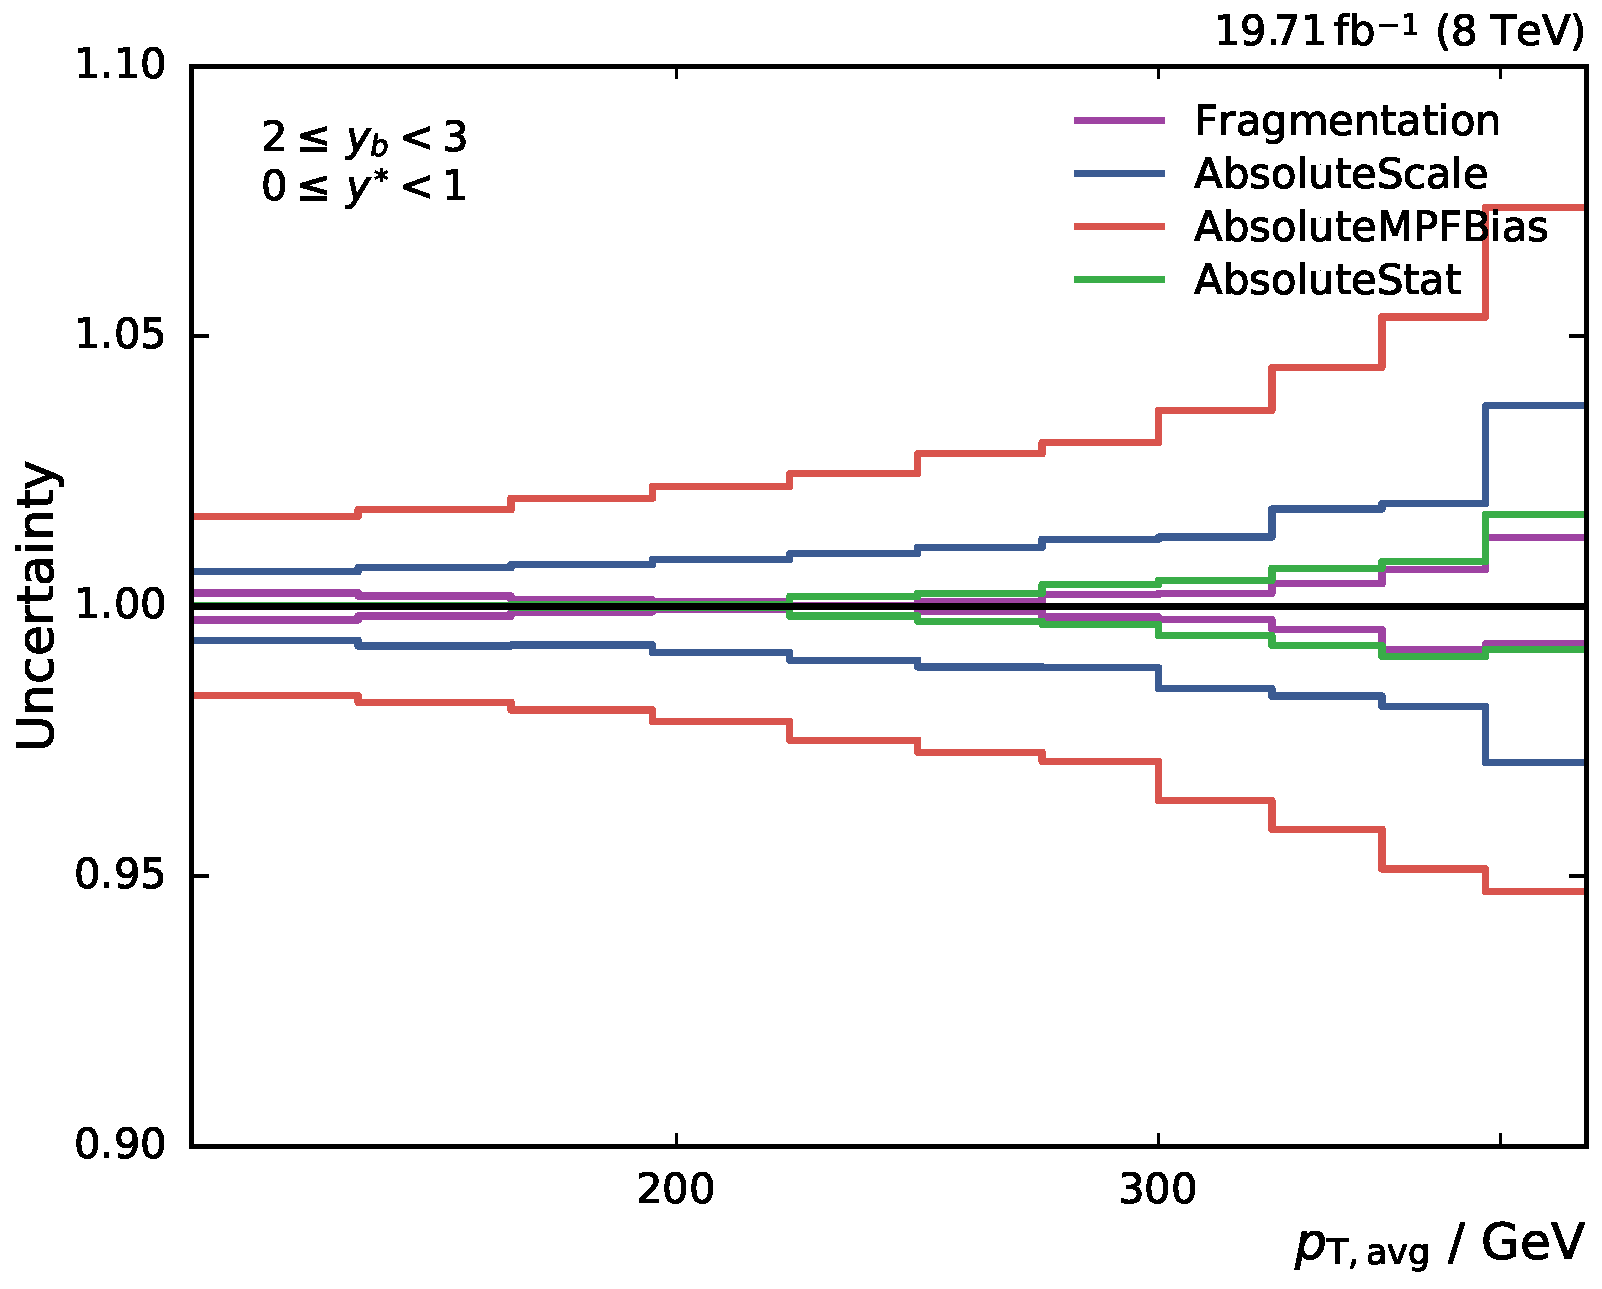
\includegraphics[width=0.45\textwidth]{figures/measurement/jec_relunc_0_yb2ys0.pdf}
    \caption{Splitup of the uncertainties due to jet energy corrections.}
    \label{fig:jec_relunc_0}
\end{figure}

\begin{figure}[htbp]
    \centering
    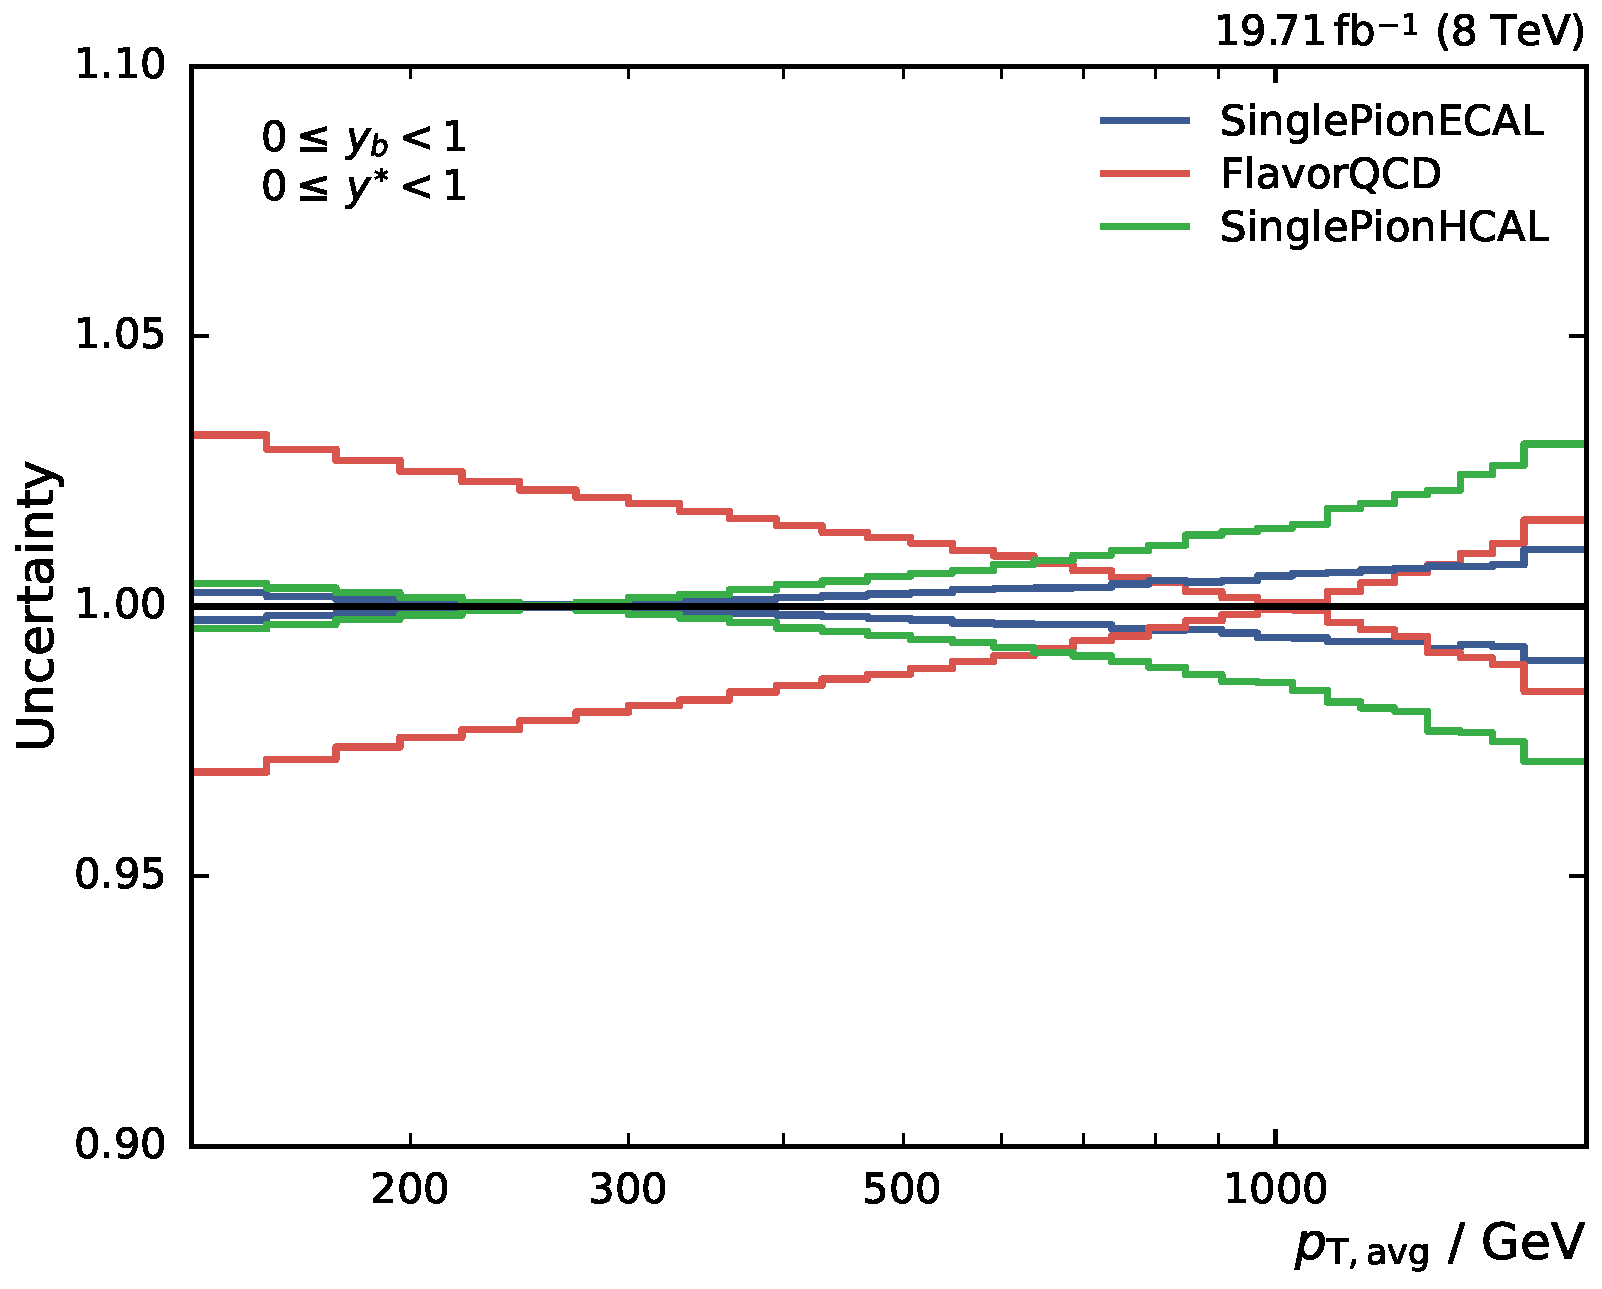
\includegraphics[width=0.45\textwidth]{figures/measurement/jec_relunc_1_yb0ys0.pdf}\hfill
    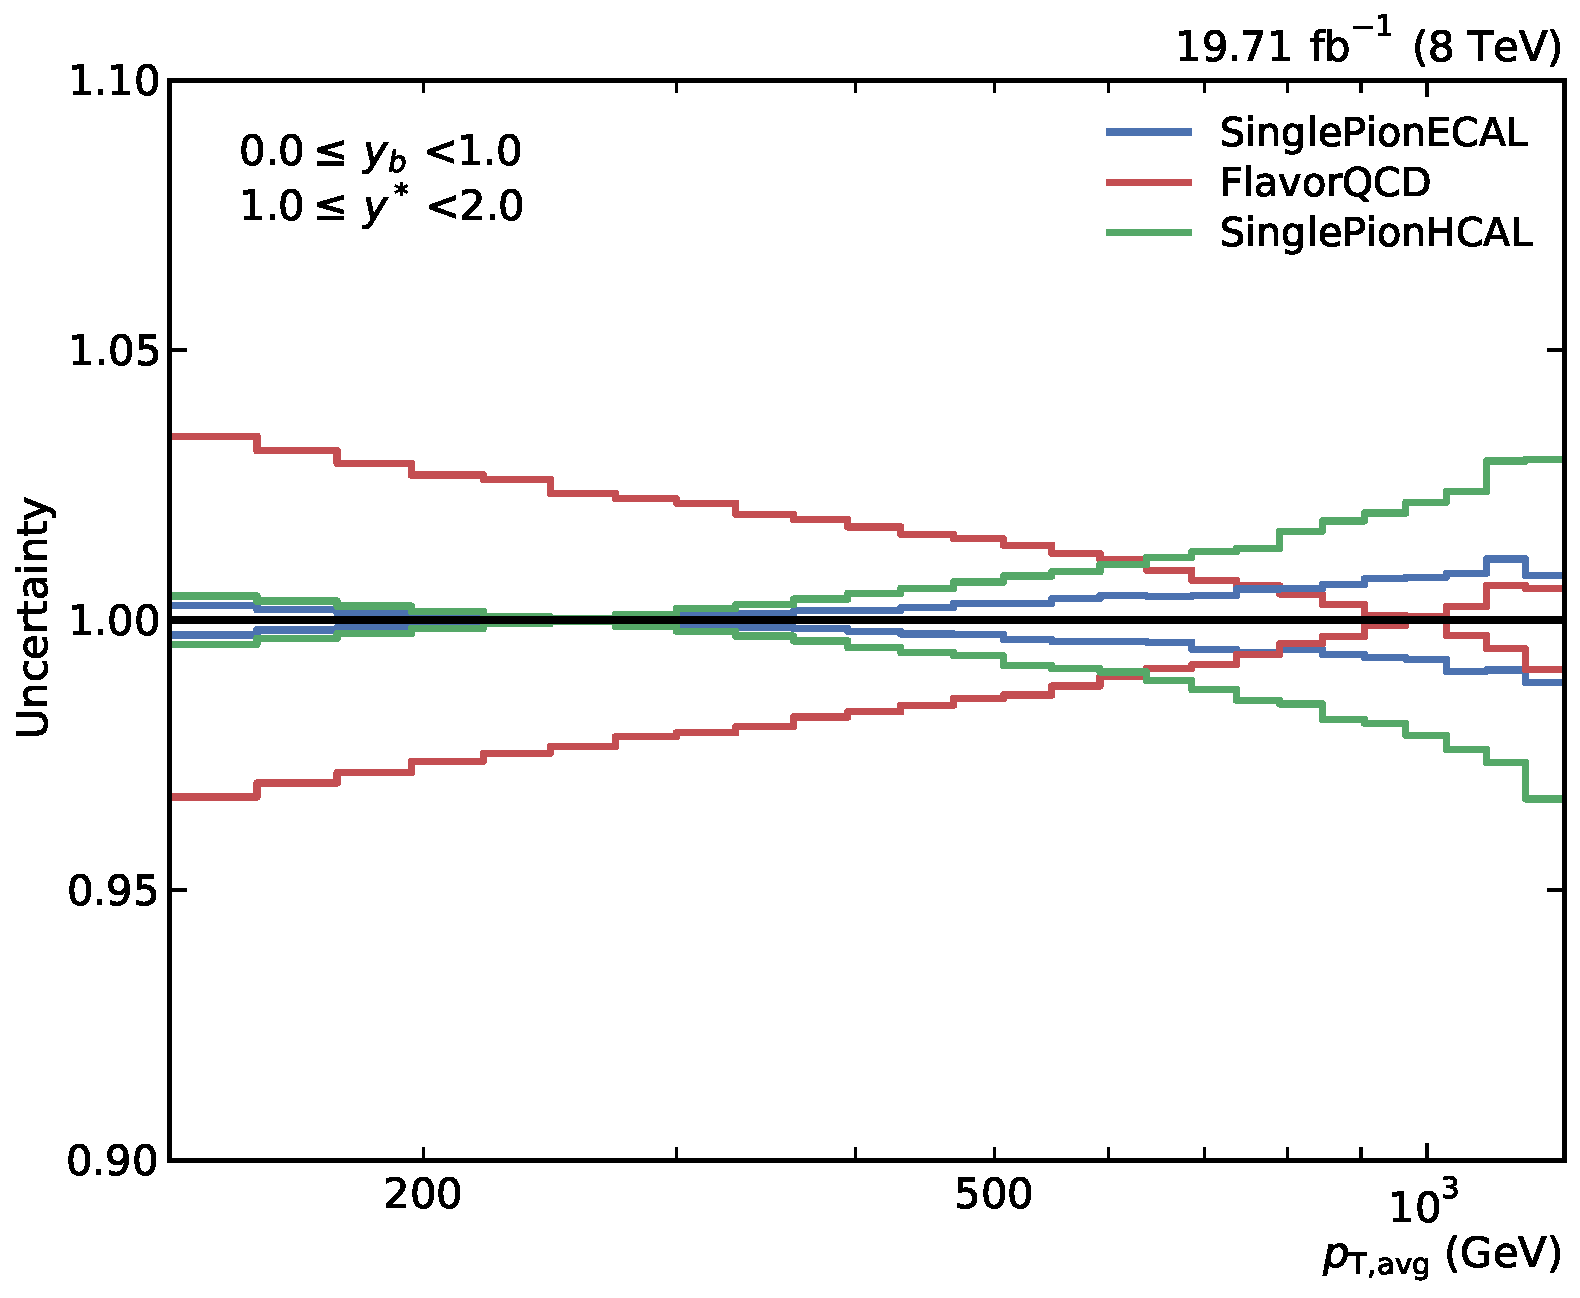
\includegraphics[width=0.45\textwidth]{figures/measurement/jec_relunc_1_yb0ys1.pdf}
    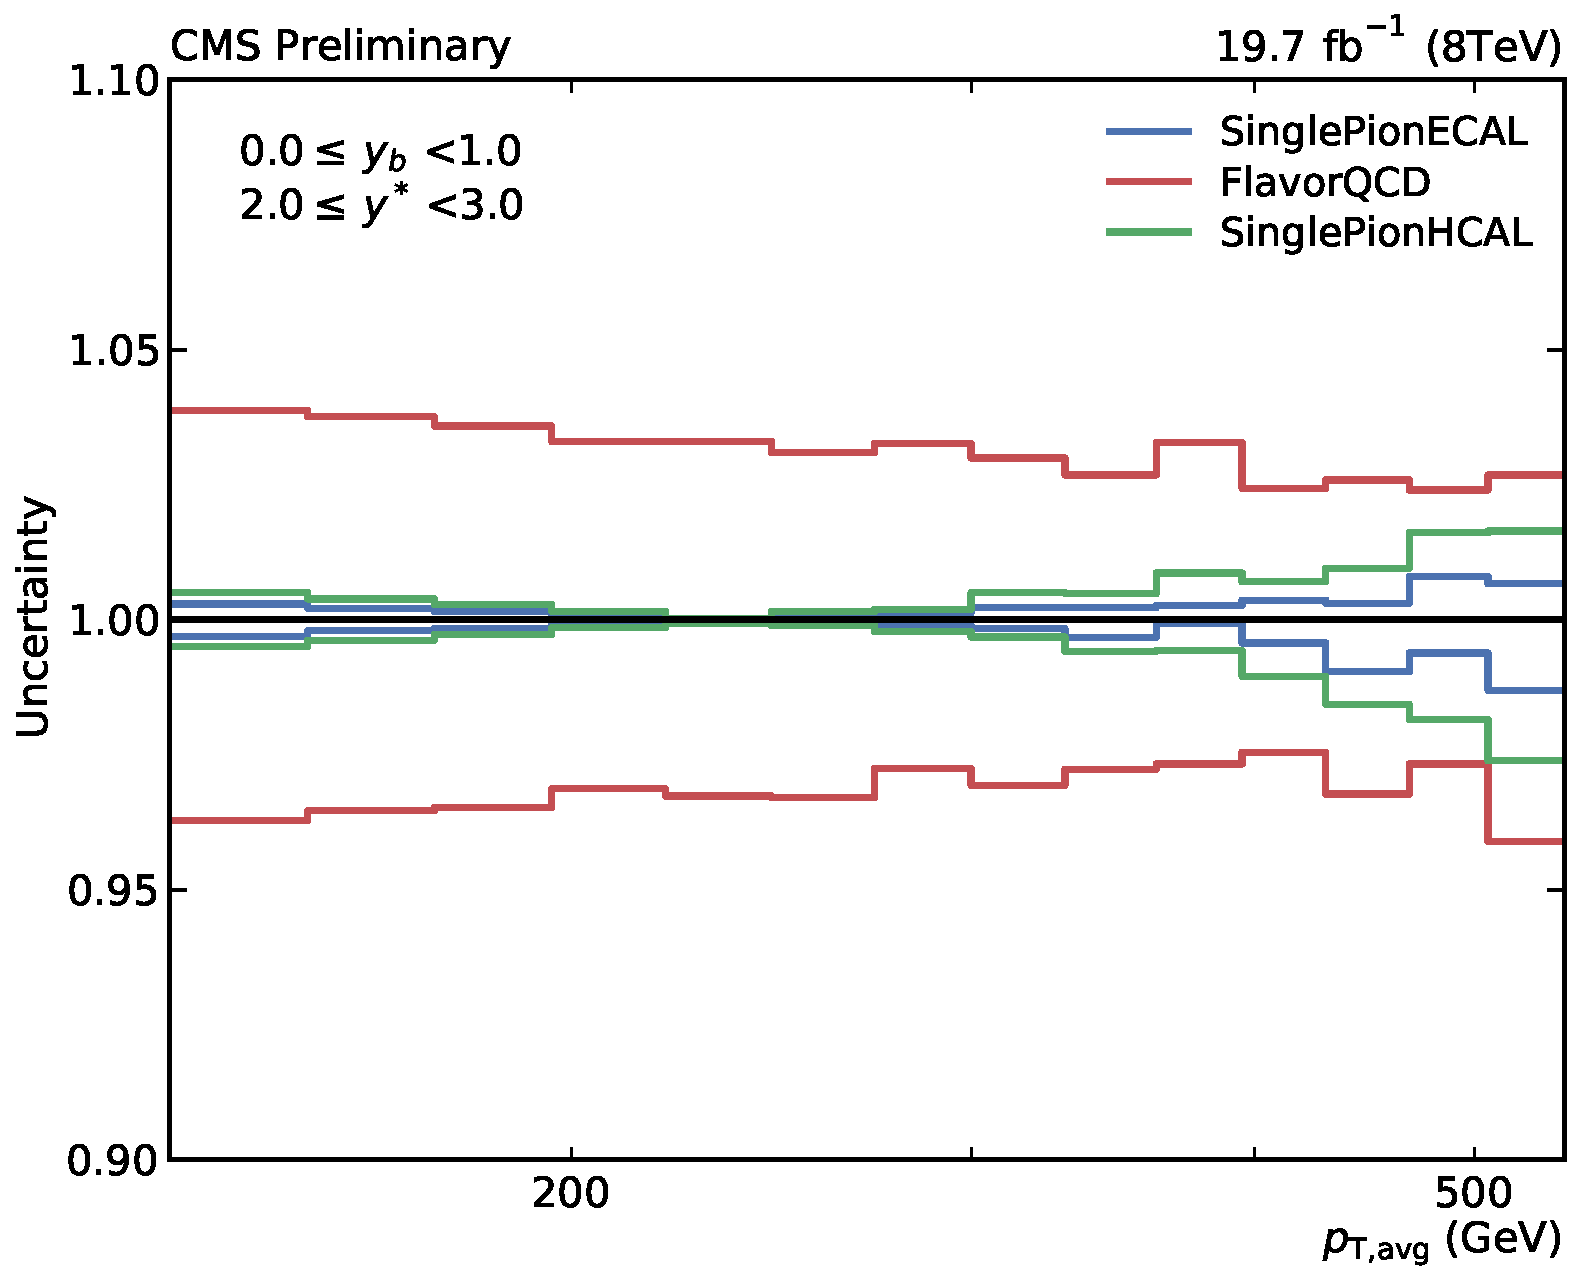
\includegraphics[width=0.45\textwidth]{figures/measurement/jec_relunc_1_yb0ys2.pdf}\hfill
    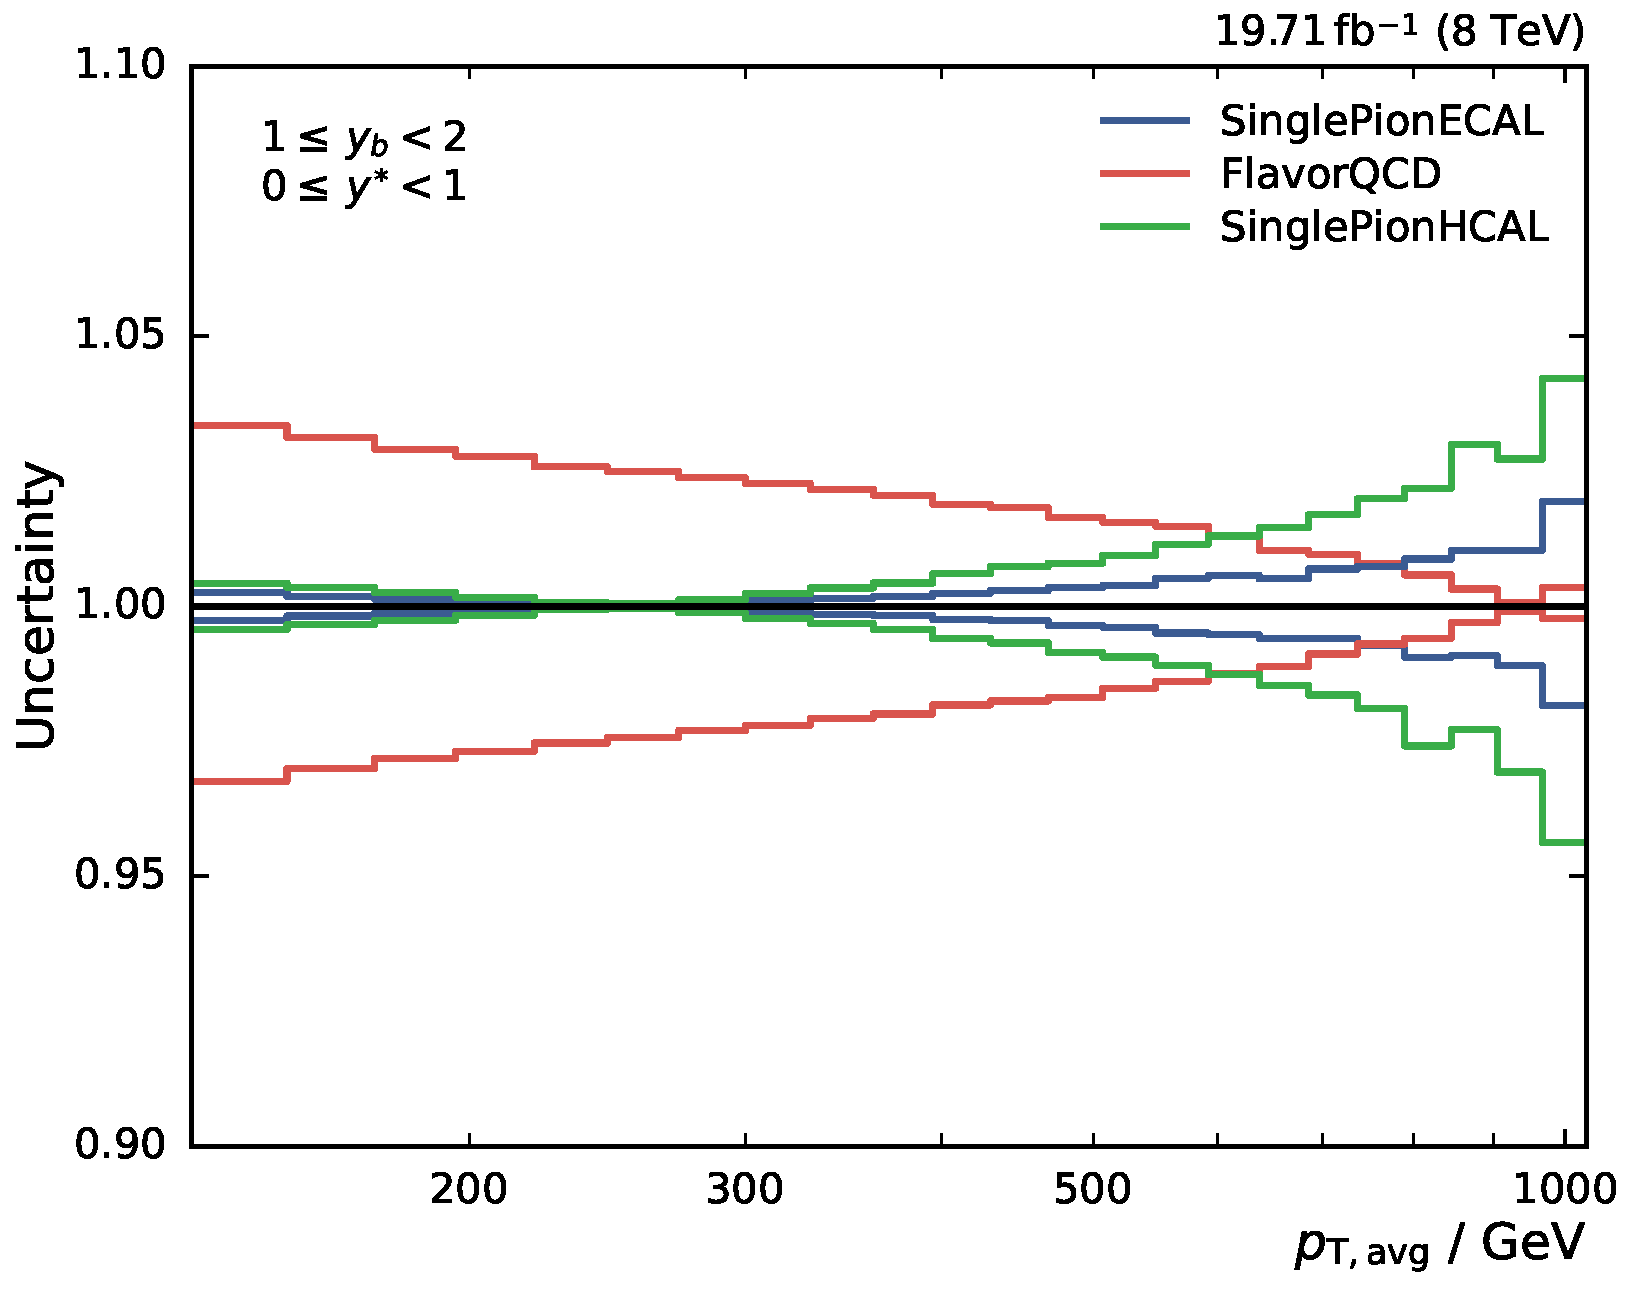
\includegraphics[width=0.45\textwidth]{figures/measurement/jec_relunc_1_yb1ys0.pdf}
    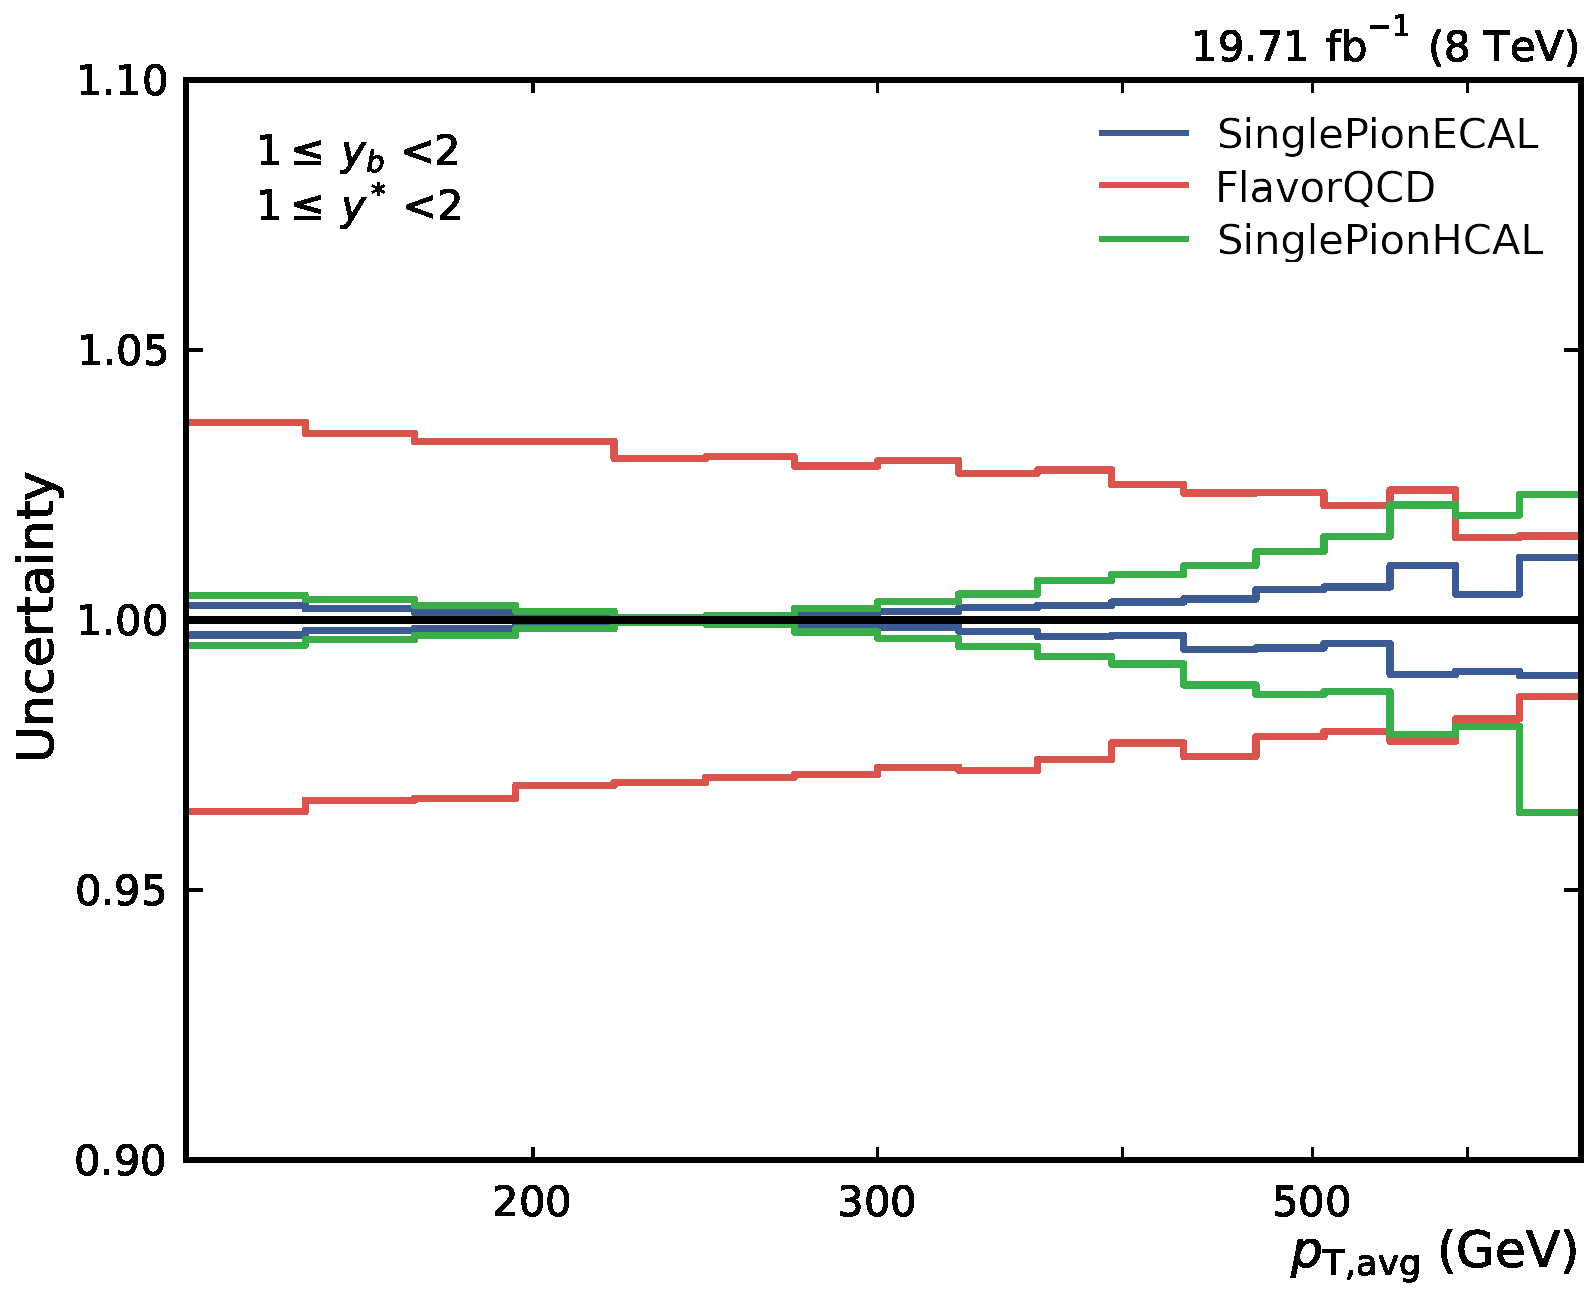
\includegraphics[width=0.45\textwidth]{figures/measurement/jec_relunc_1_yb1ys1.pdf}\hfill
    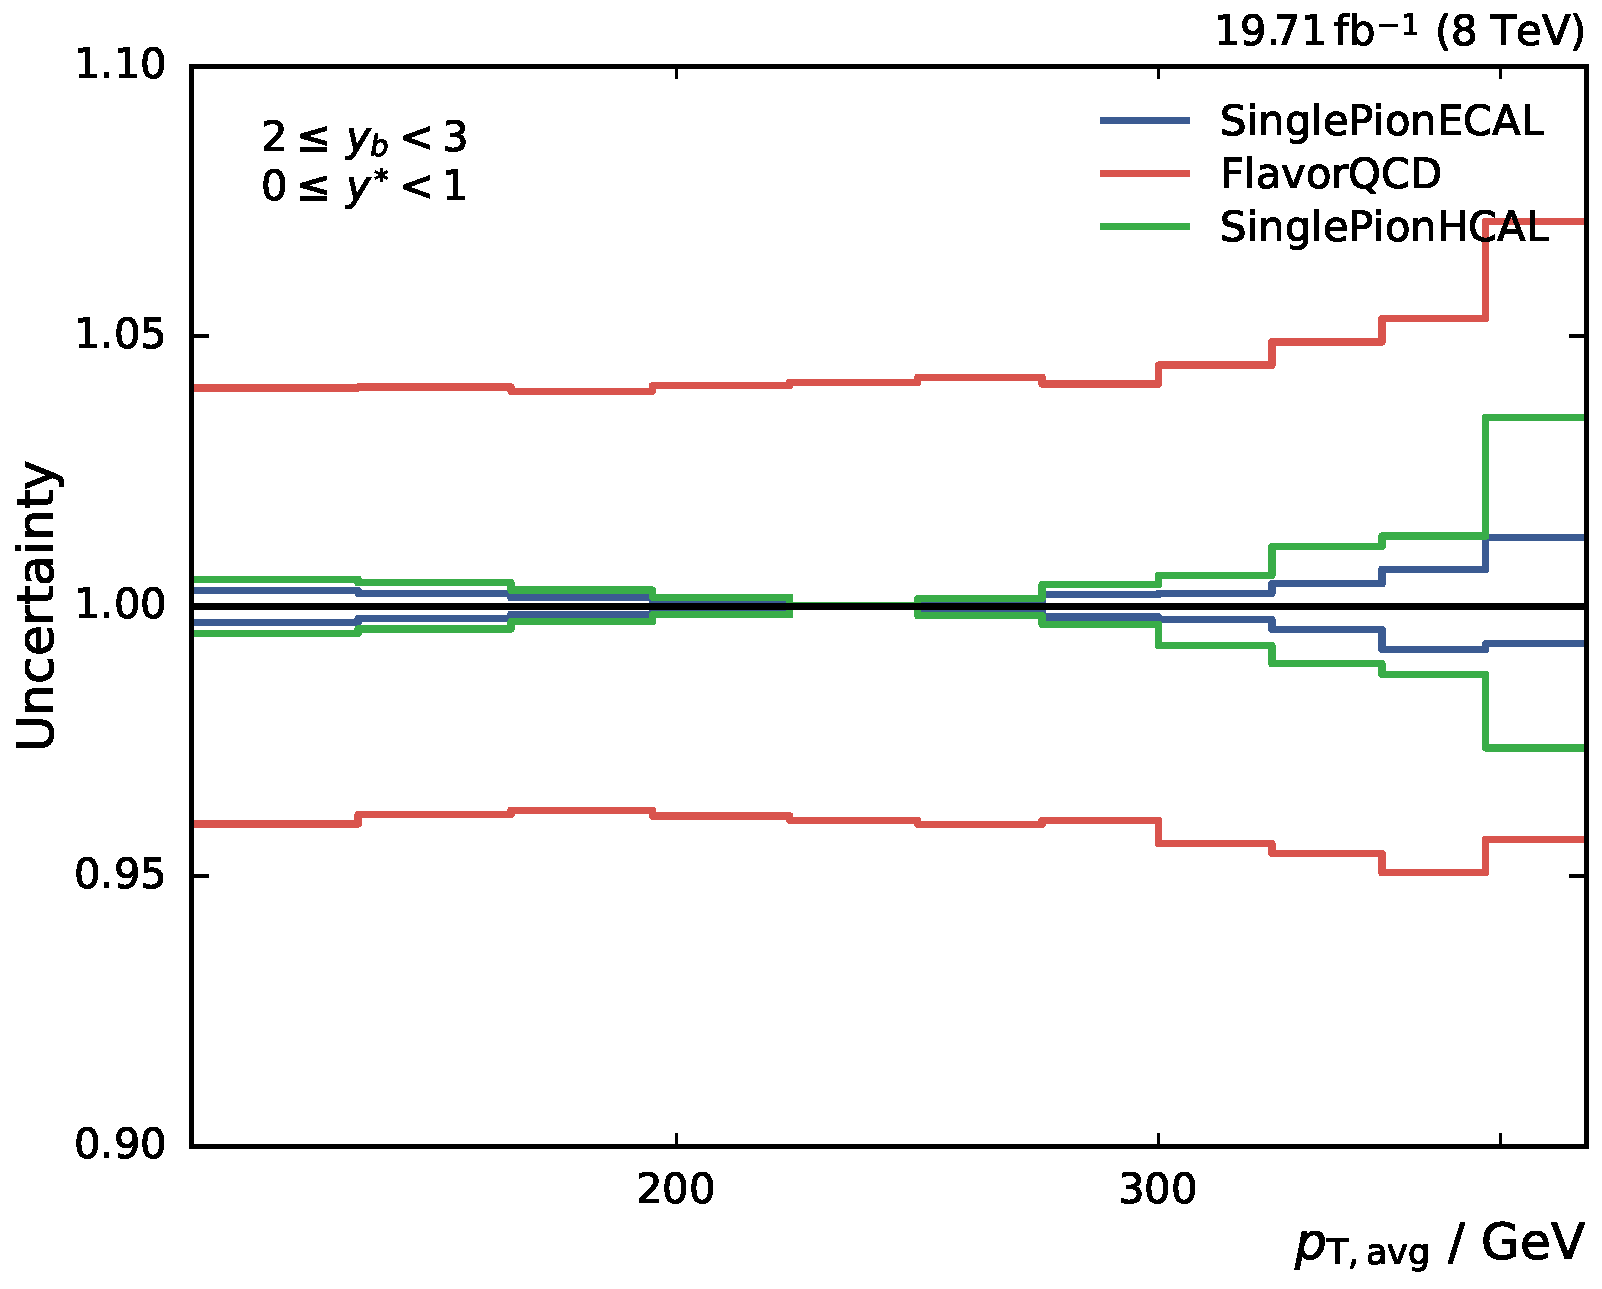
\includegraphics[width=0.45\textwidth]{figures/measurement/jec_relunc_1_yb2ys0.pdf}
    \caption{Splitup of the uncertainties due to jet energy corrections.}
    \label{fig:jec_relunc_1}
\end{figure}

\begin{figure}[htbp]
    \centering
    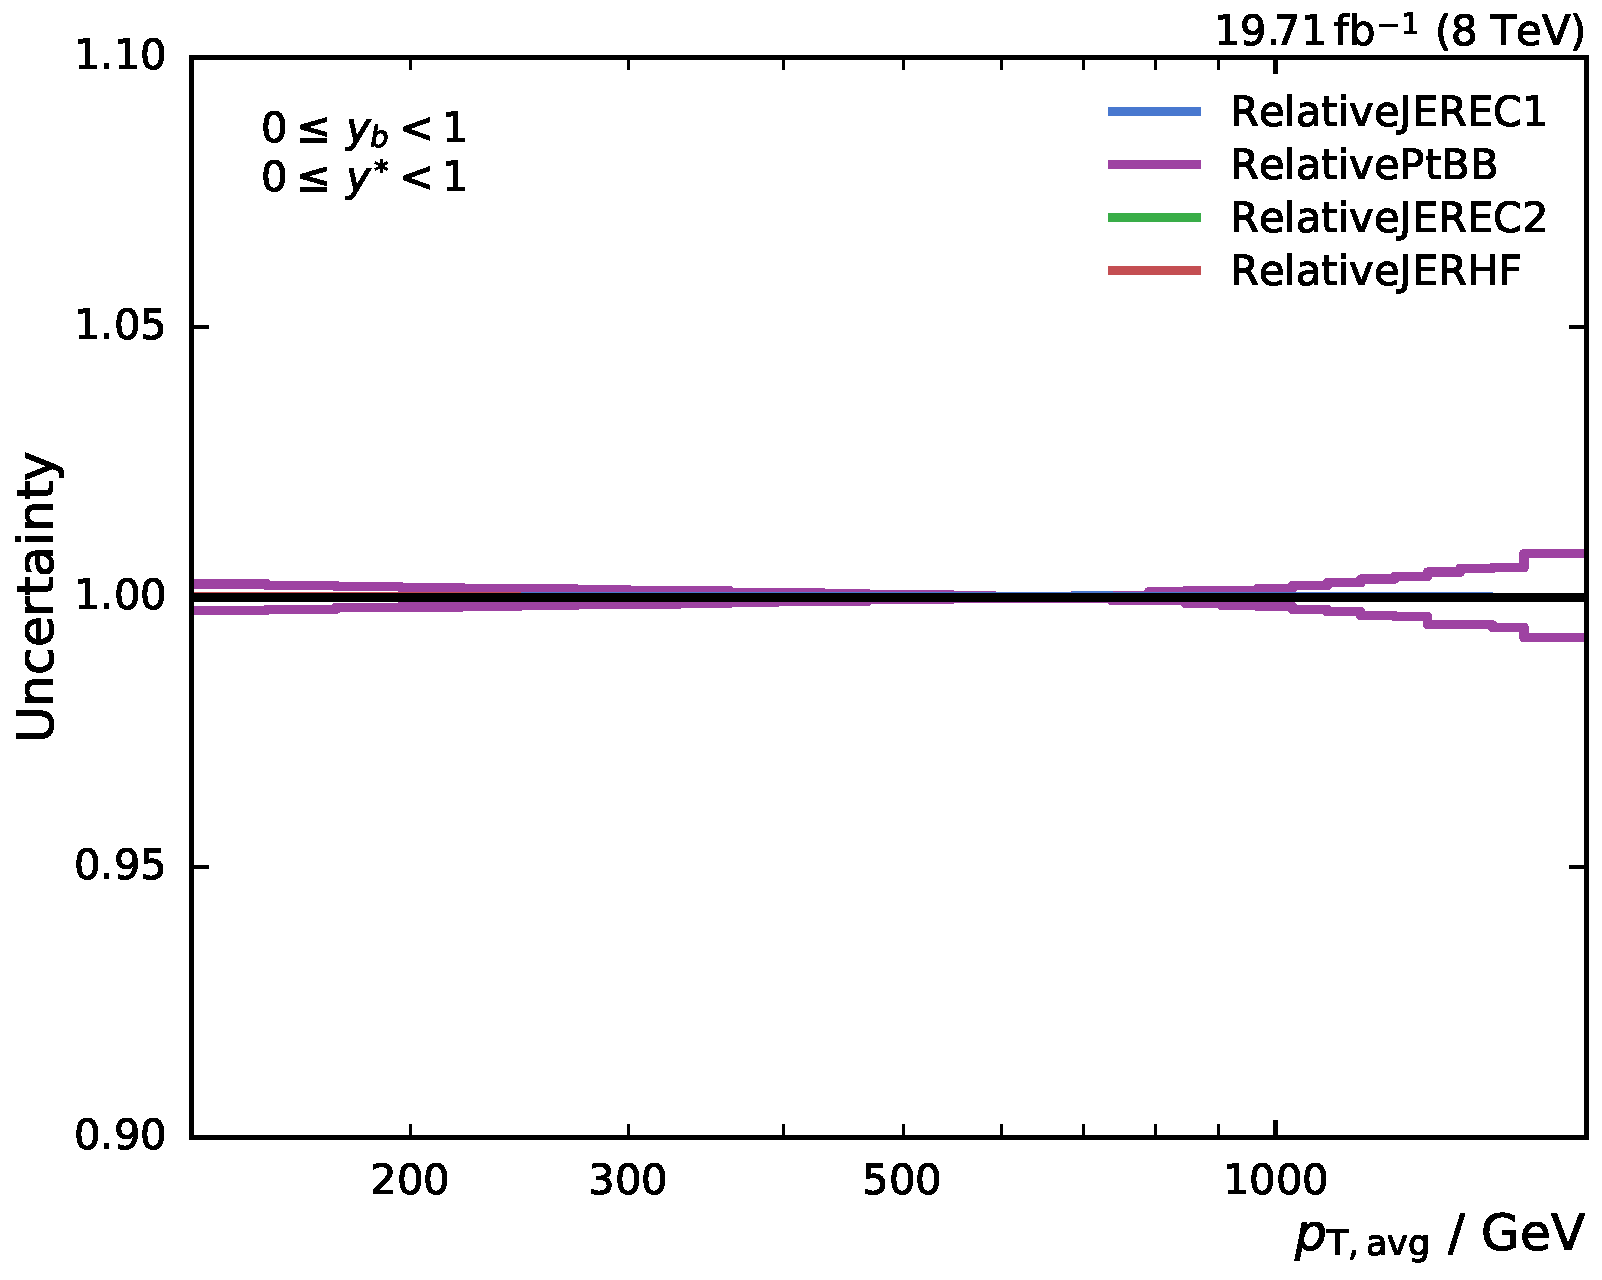
\includegraphics[width=0.45\textwidth]{figures/measurement/jec_relunc_2_yb0ys0.pdf}\hfill
    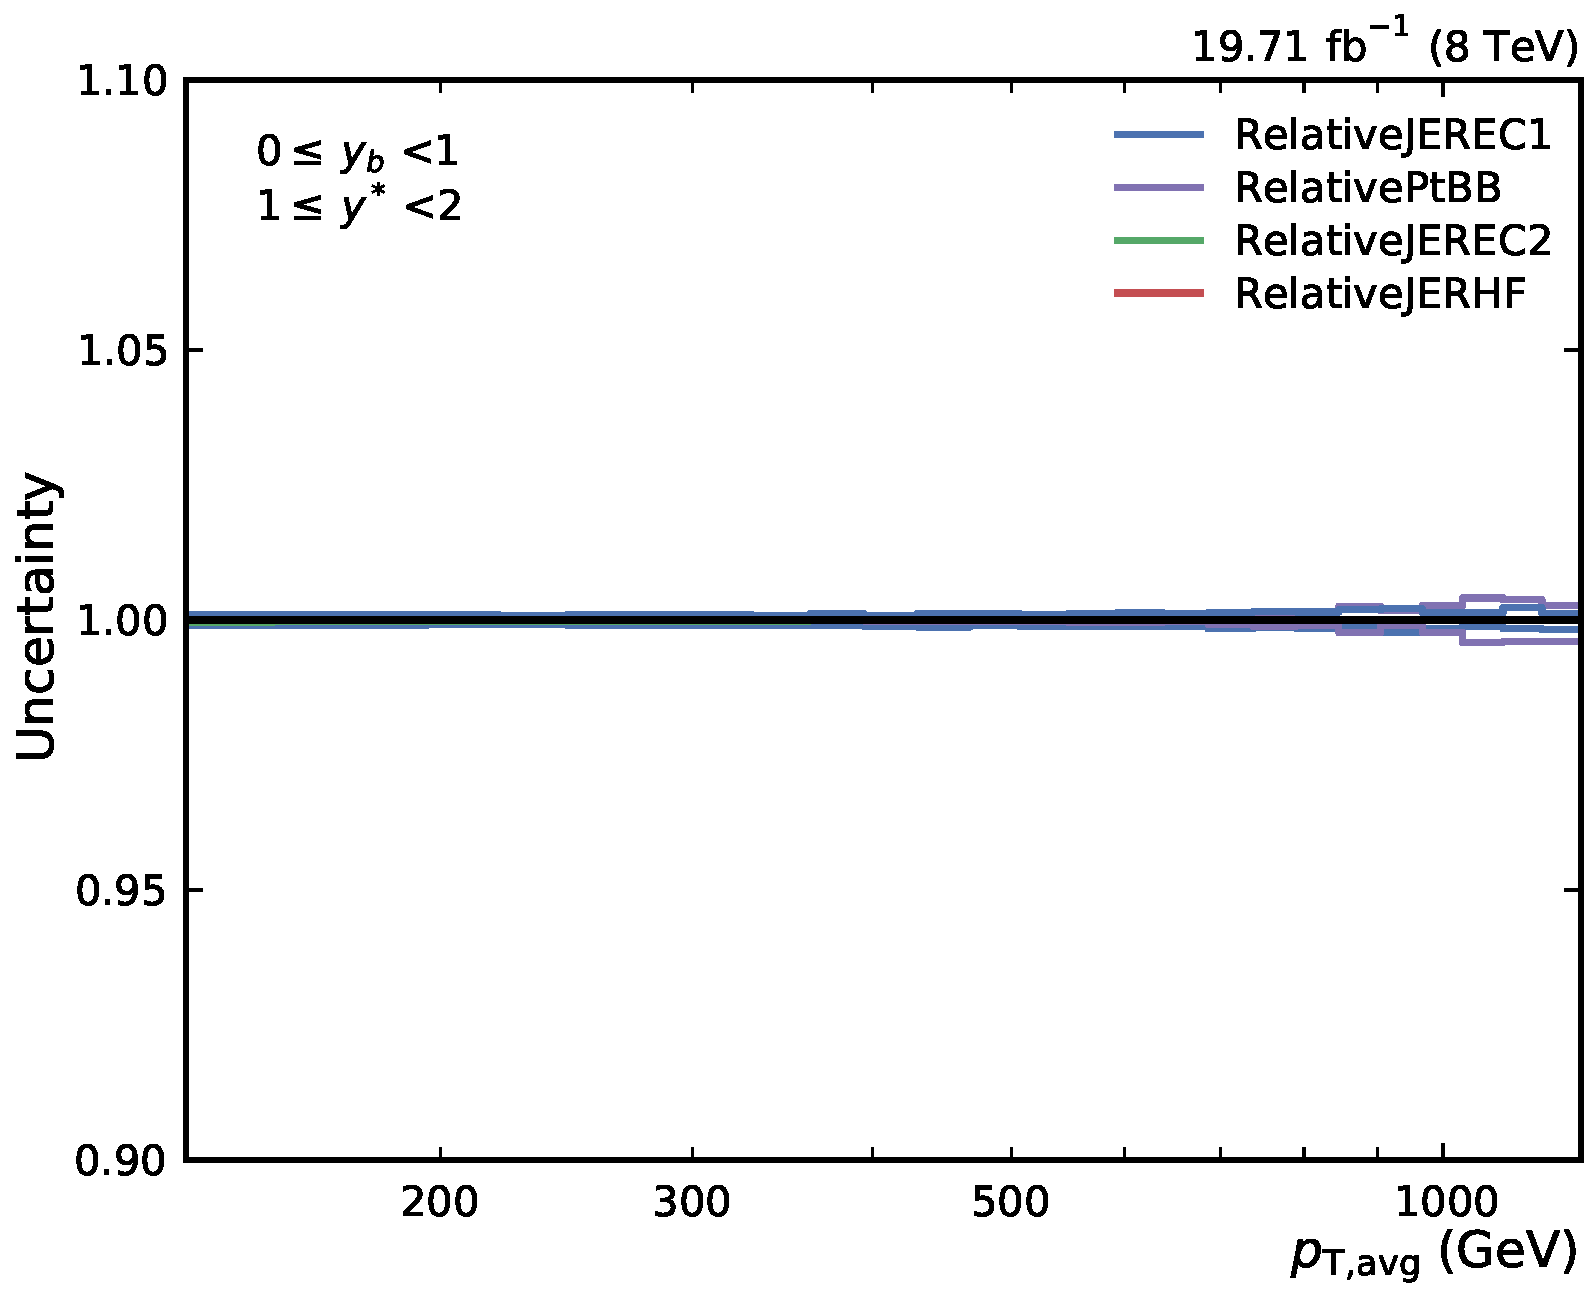
\includegraphics[width=0.45\textwidth]{figures/measurement/jec_relunc_2_yb0ys1.pdf}
    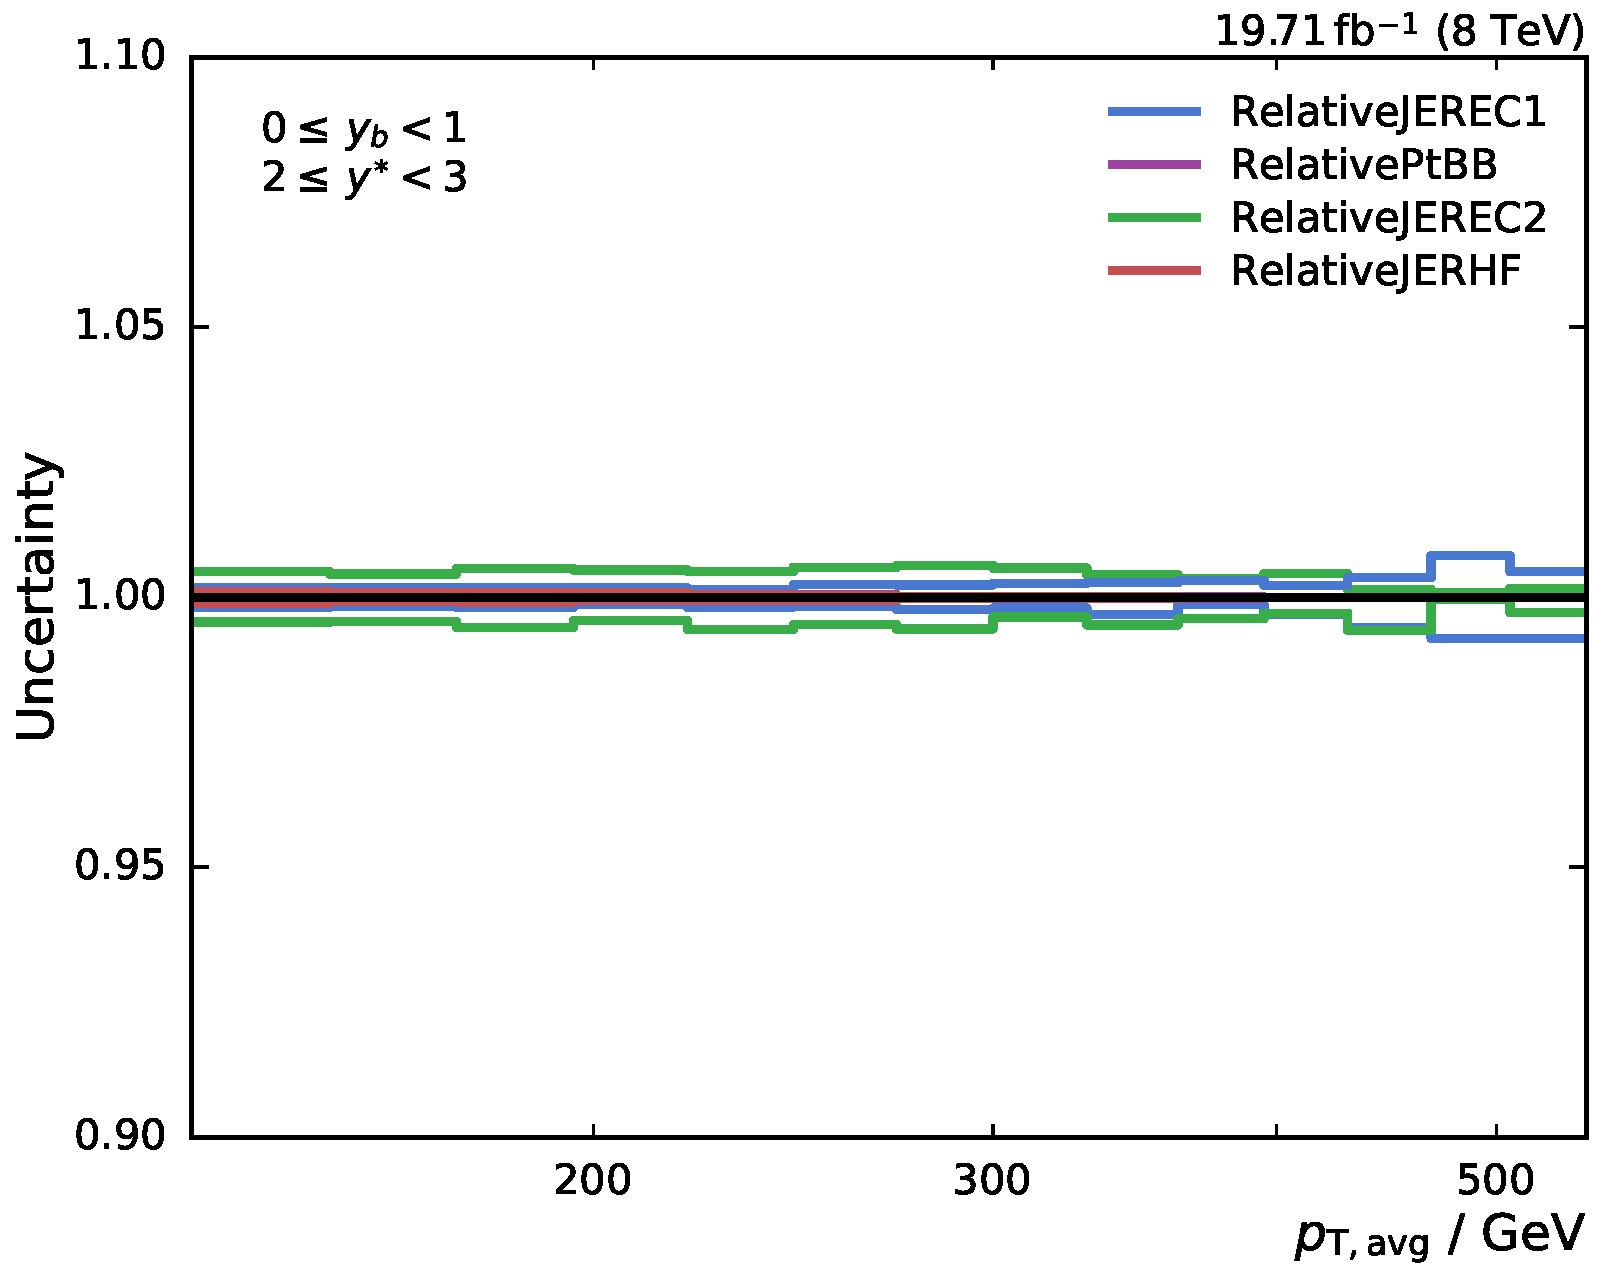
\includegraphics[width=0.45\textwidth]{figures/measurement/jec_relunc_2_yb0ys2.pdf}\hfill
    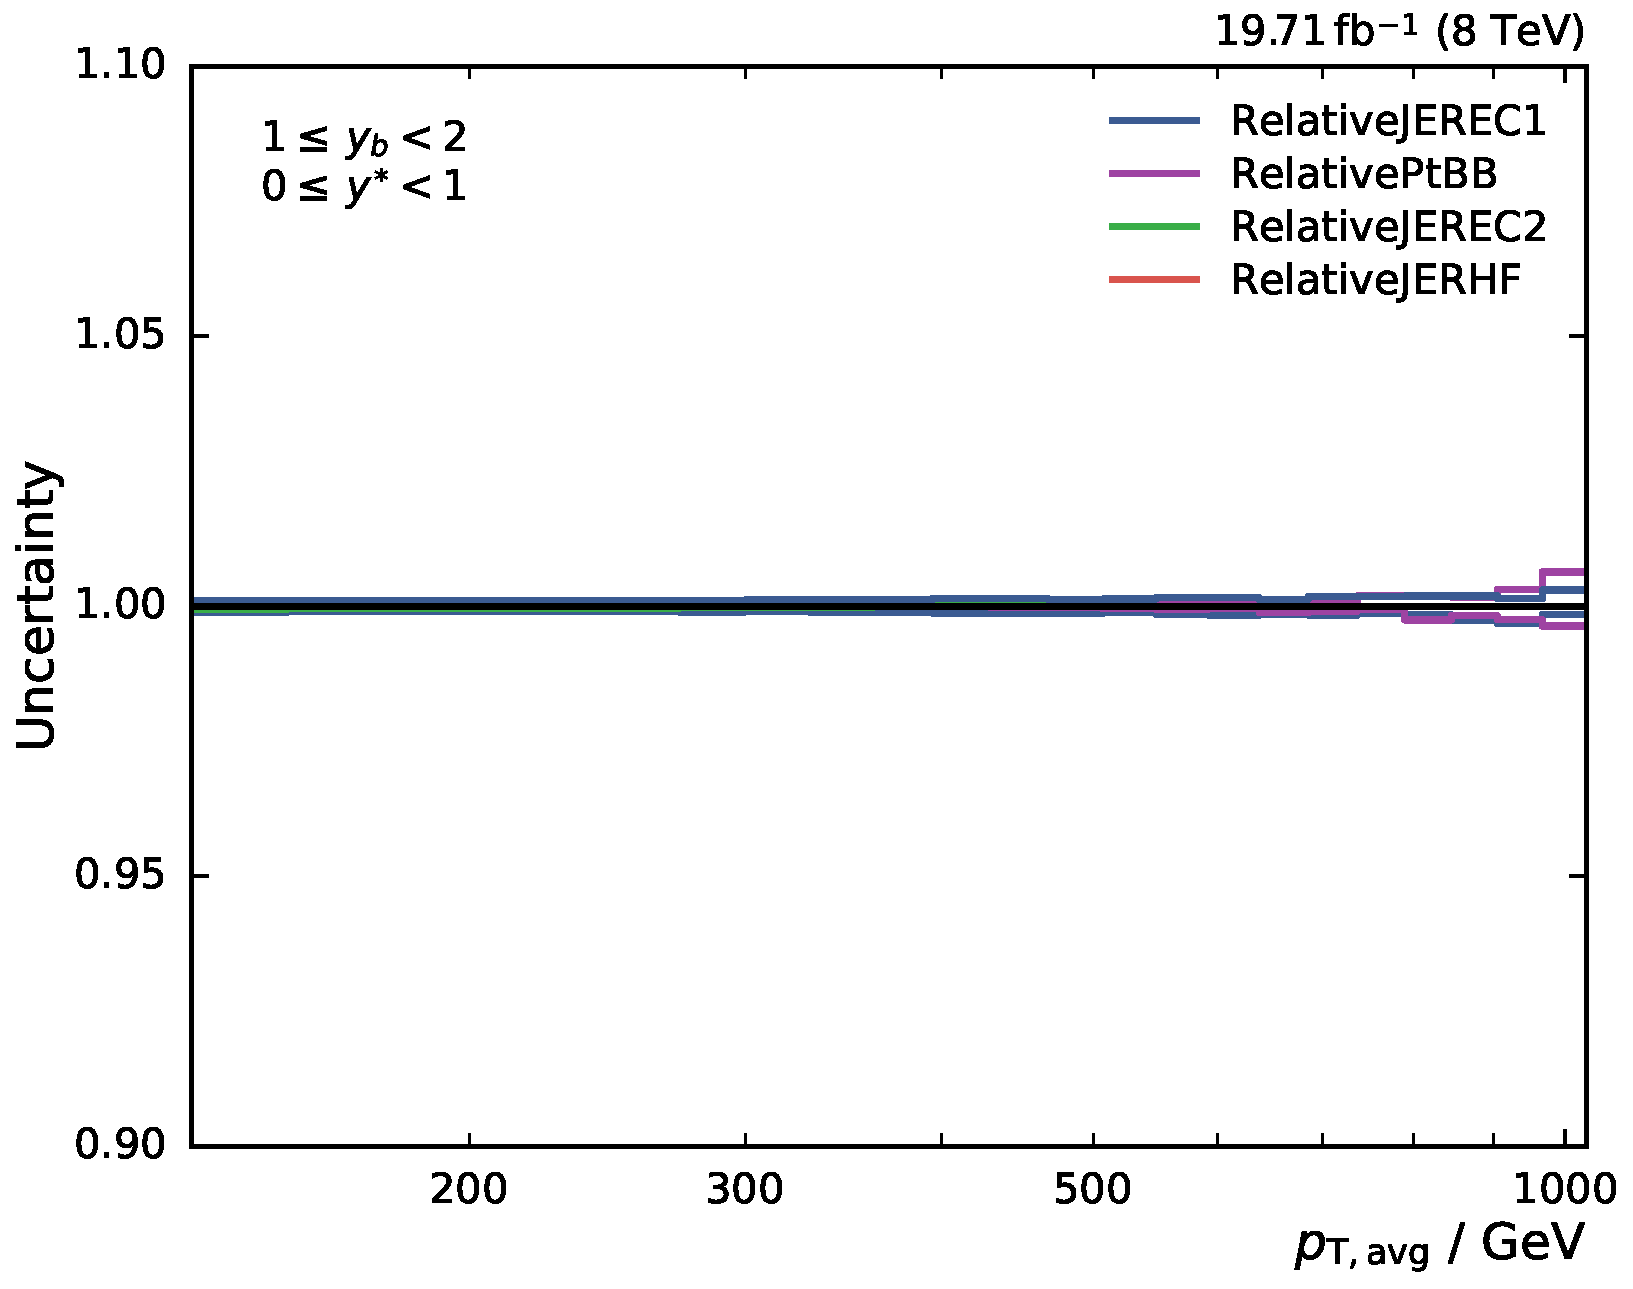
\includegraphics[width=0.45\textwidth]{figures/measurement/jec_relunc_2_yb1ys0.pdf}
    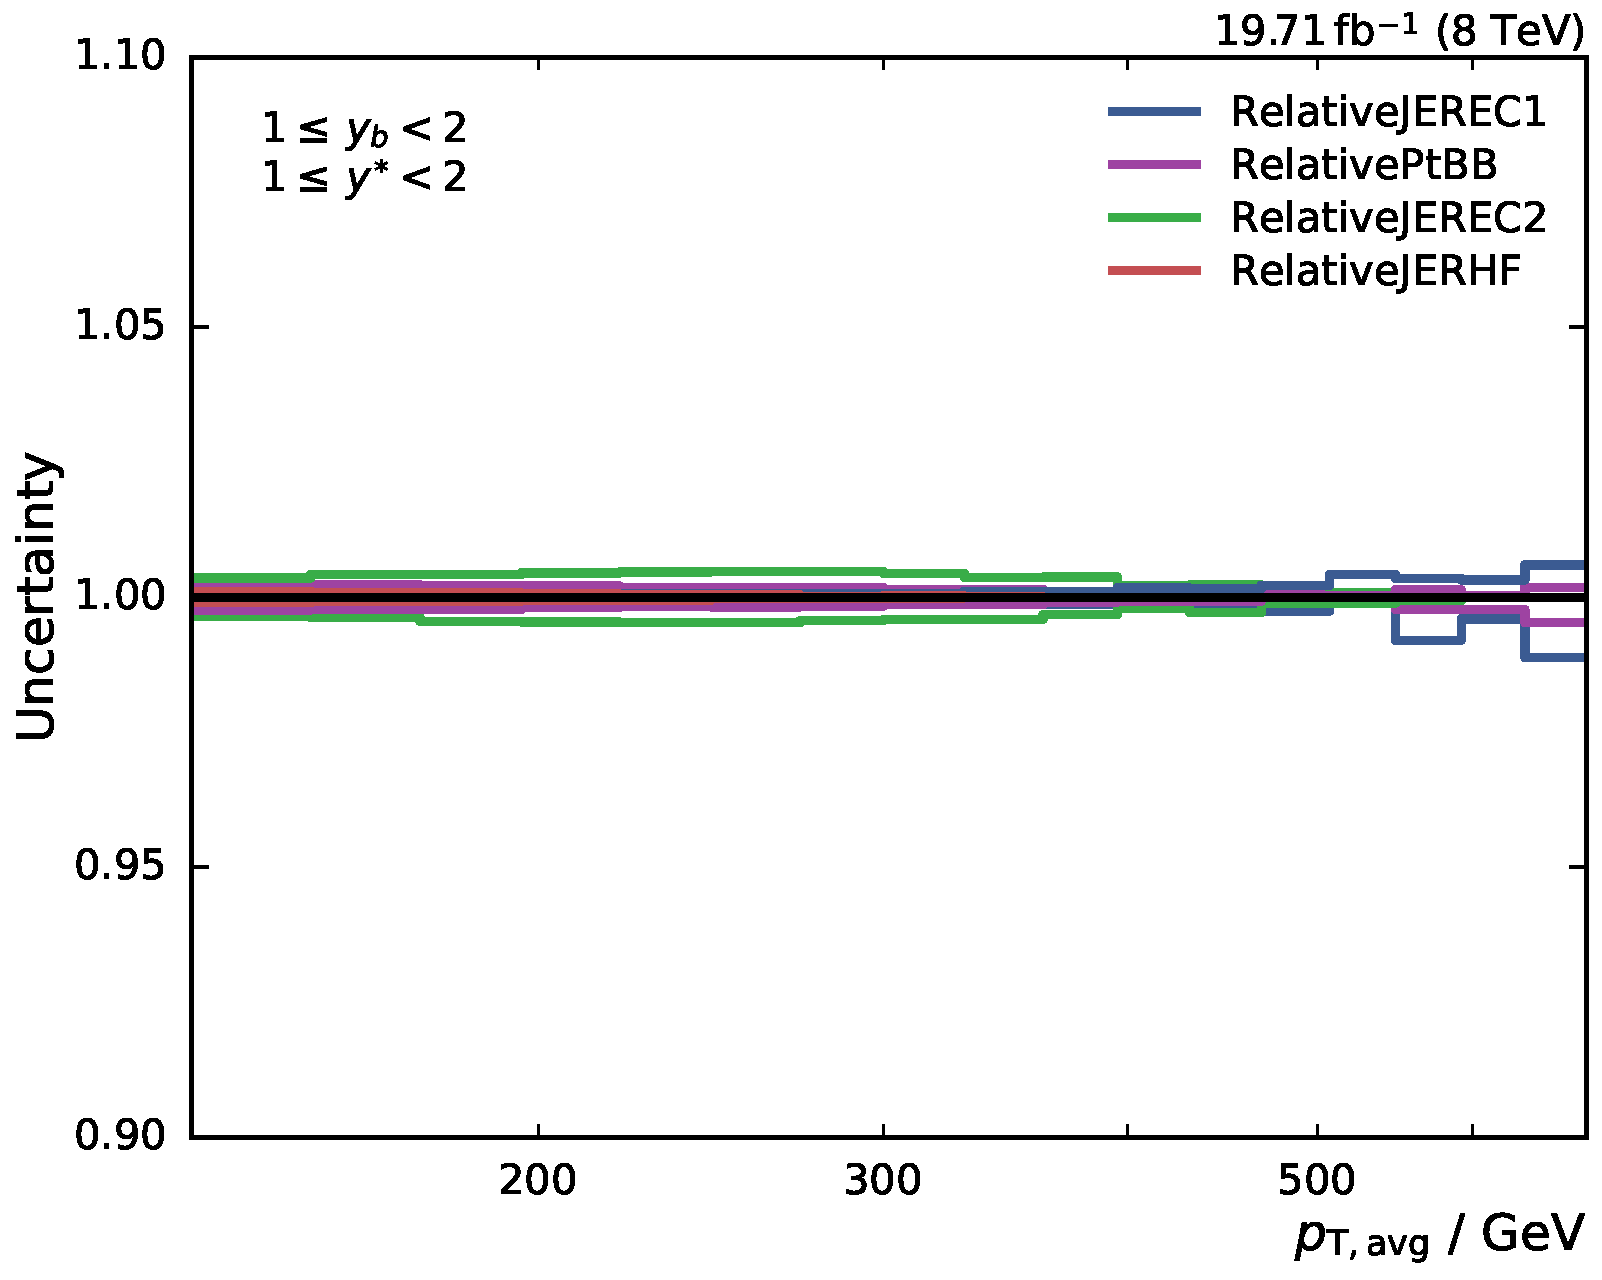
\includegraphics[width=0.45\textwidth]{figures/measurement/jec_relunc_2_yb1ys1.pdf}\hfill
    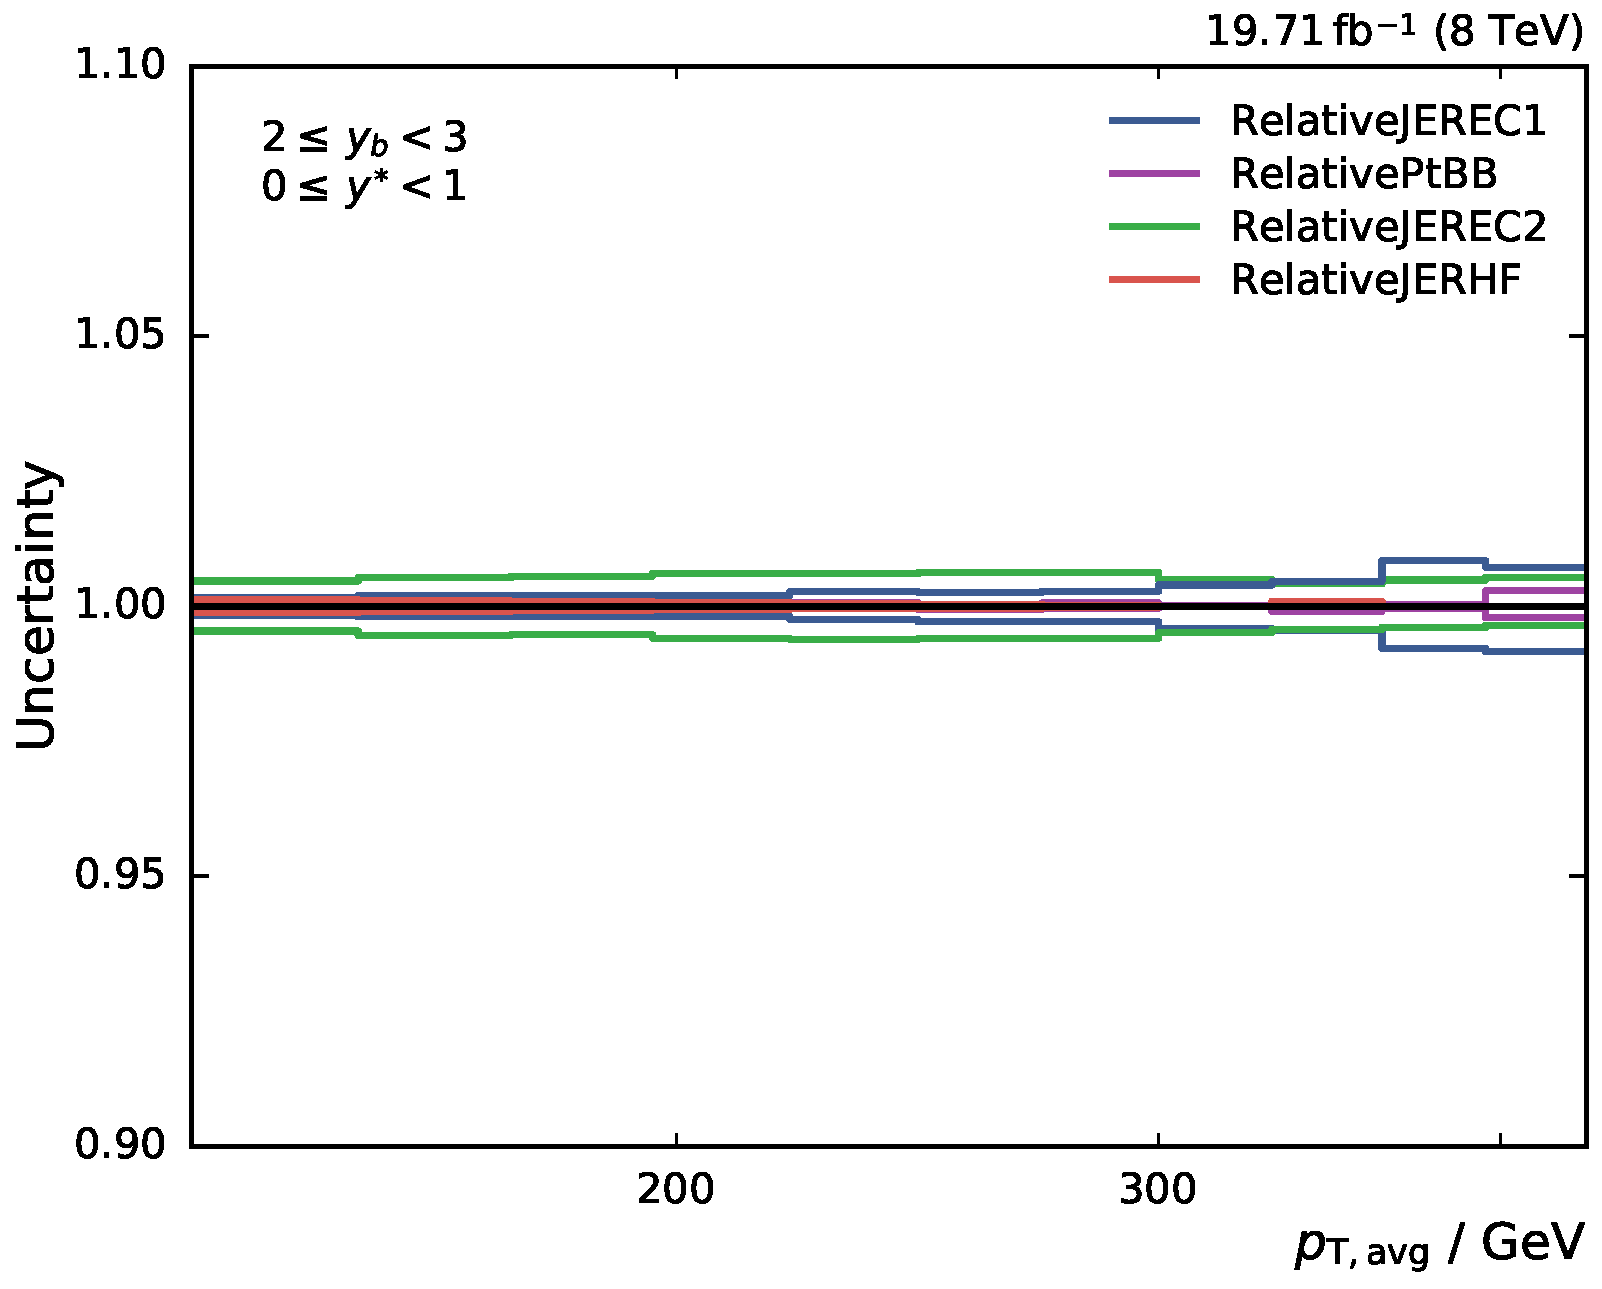
\includegraphics[width=0.45\textwidth]{figures/measurement/jec_relunc_2_yb2ys0.pdf}
    \caption{Splitup of the uncertainties due to jet energy corrections.}
    \label{fig:jec_relunc_2}
\end{figure}


\begin{figure}[htbp]
    \centering
    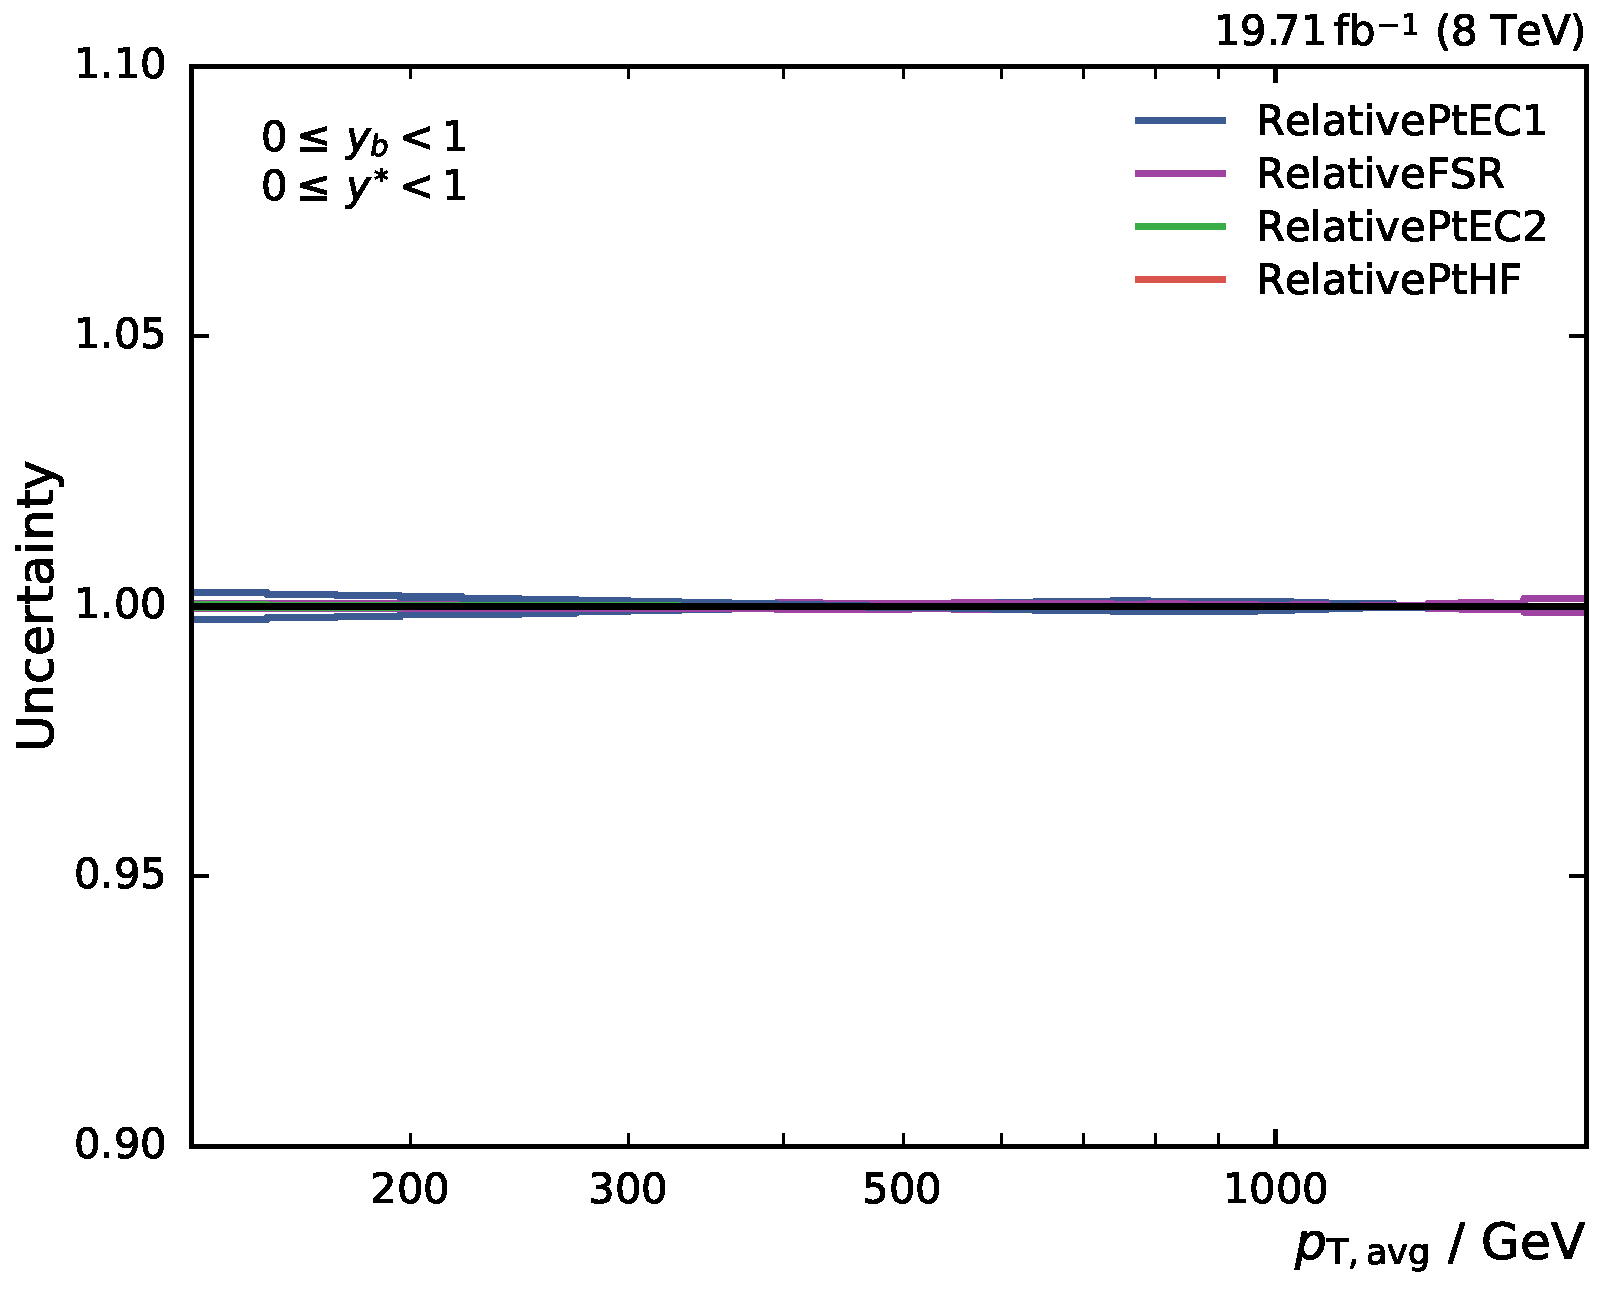
\includegraphics[width=0.45\textwidth]{figures/measurement/jec_relunc_3_yb0ys0.pdf}\hfill
    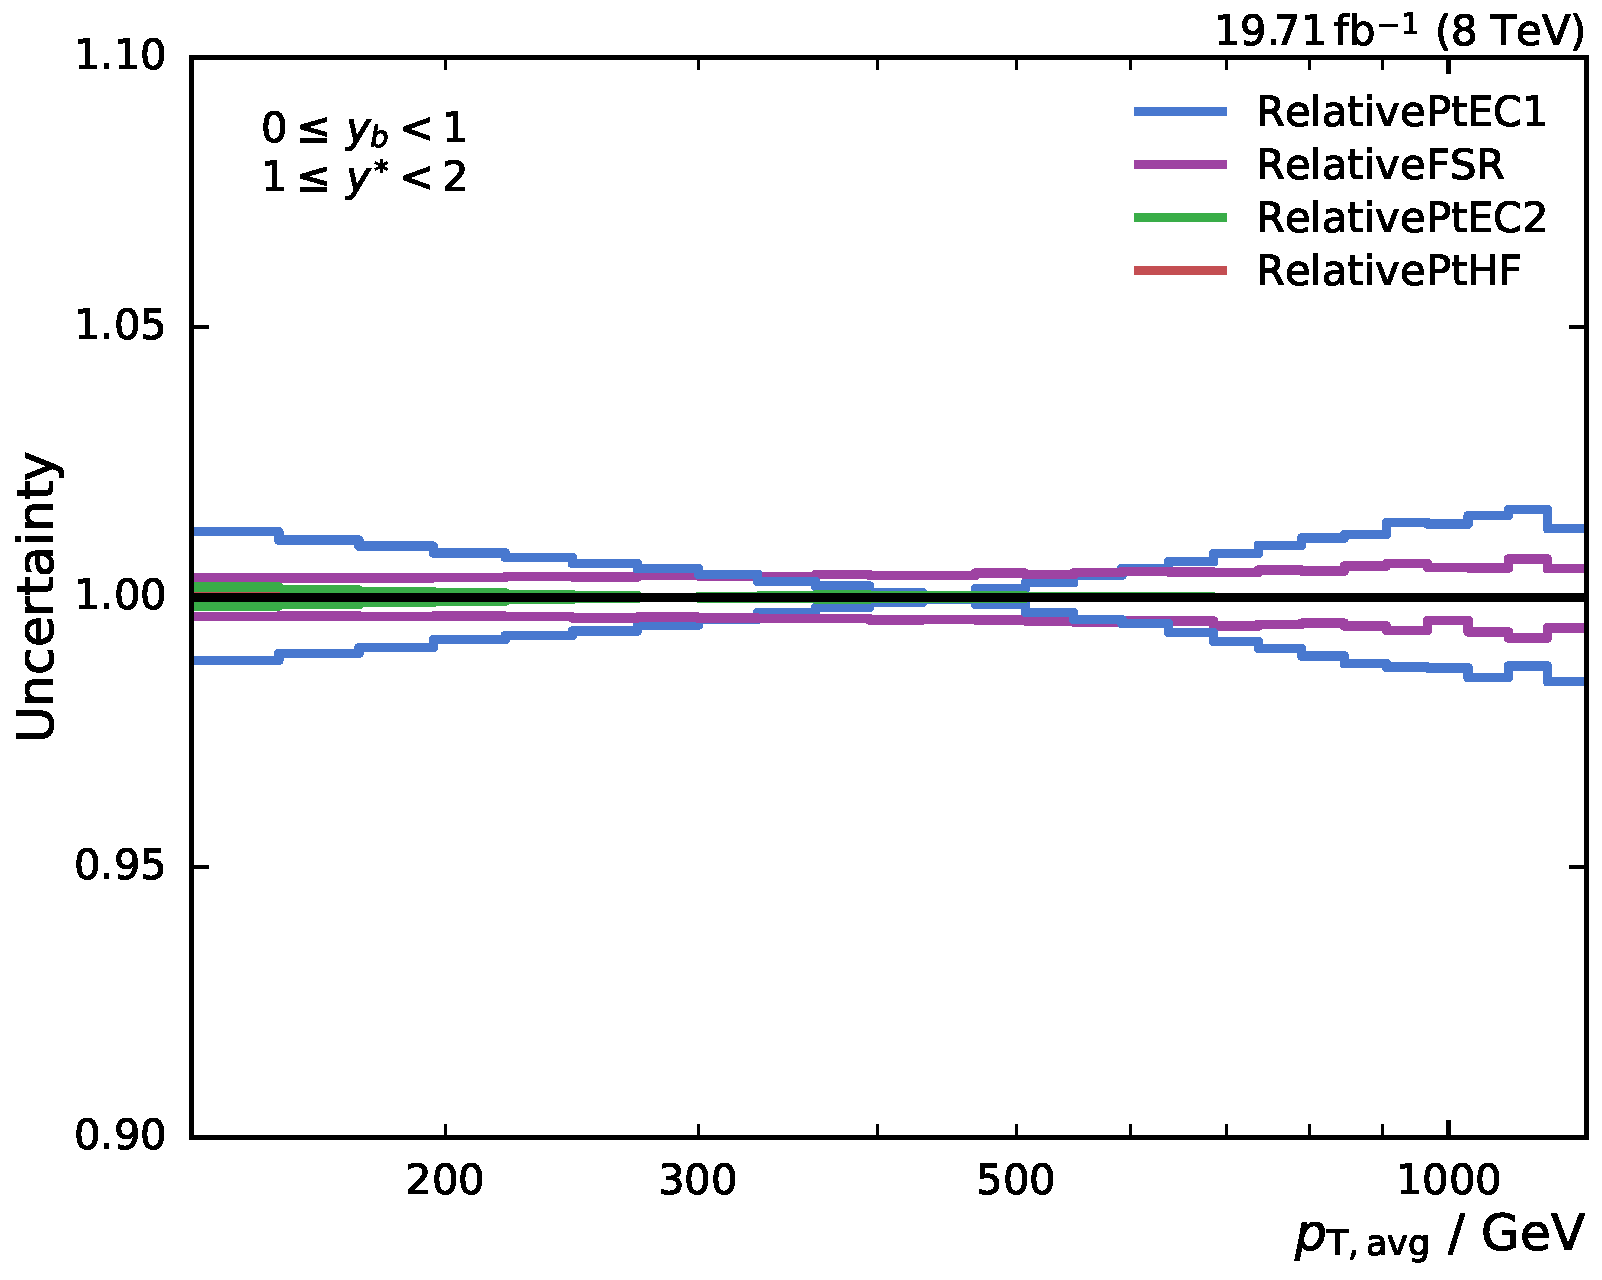
\includegraphics[width=0.45\textwidth]{figures/measurement/jec_relunc_3_yb0ys1.pdf}
    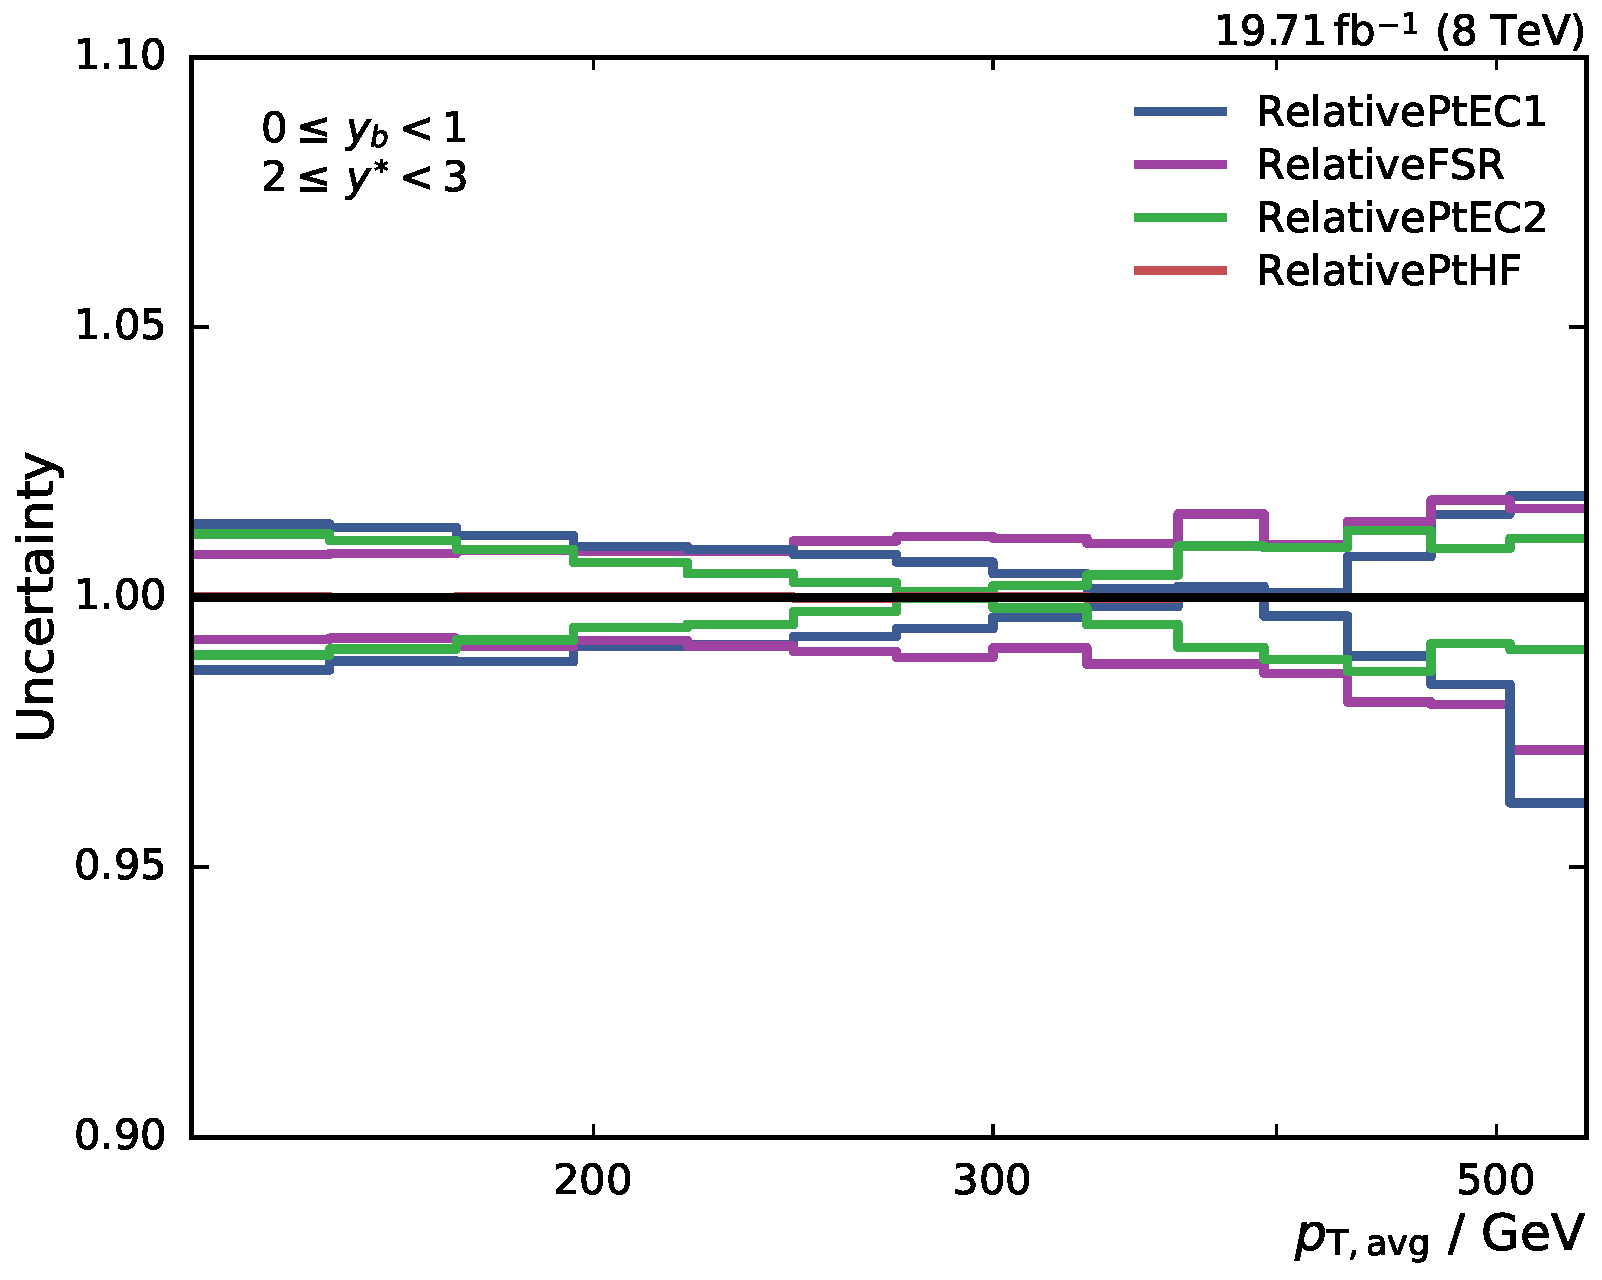
\includegraphics[width=0.45\textwidth]{figures/measurement/jec_relunc_3_yb0ys2.pdf}\hfill
    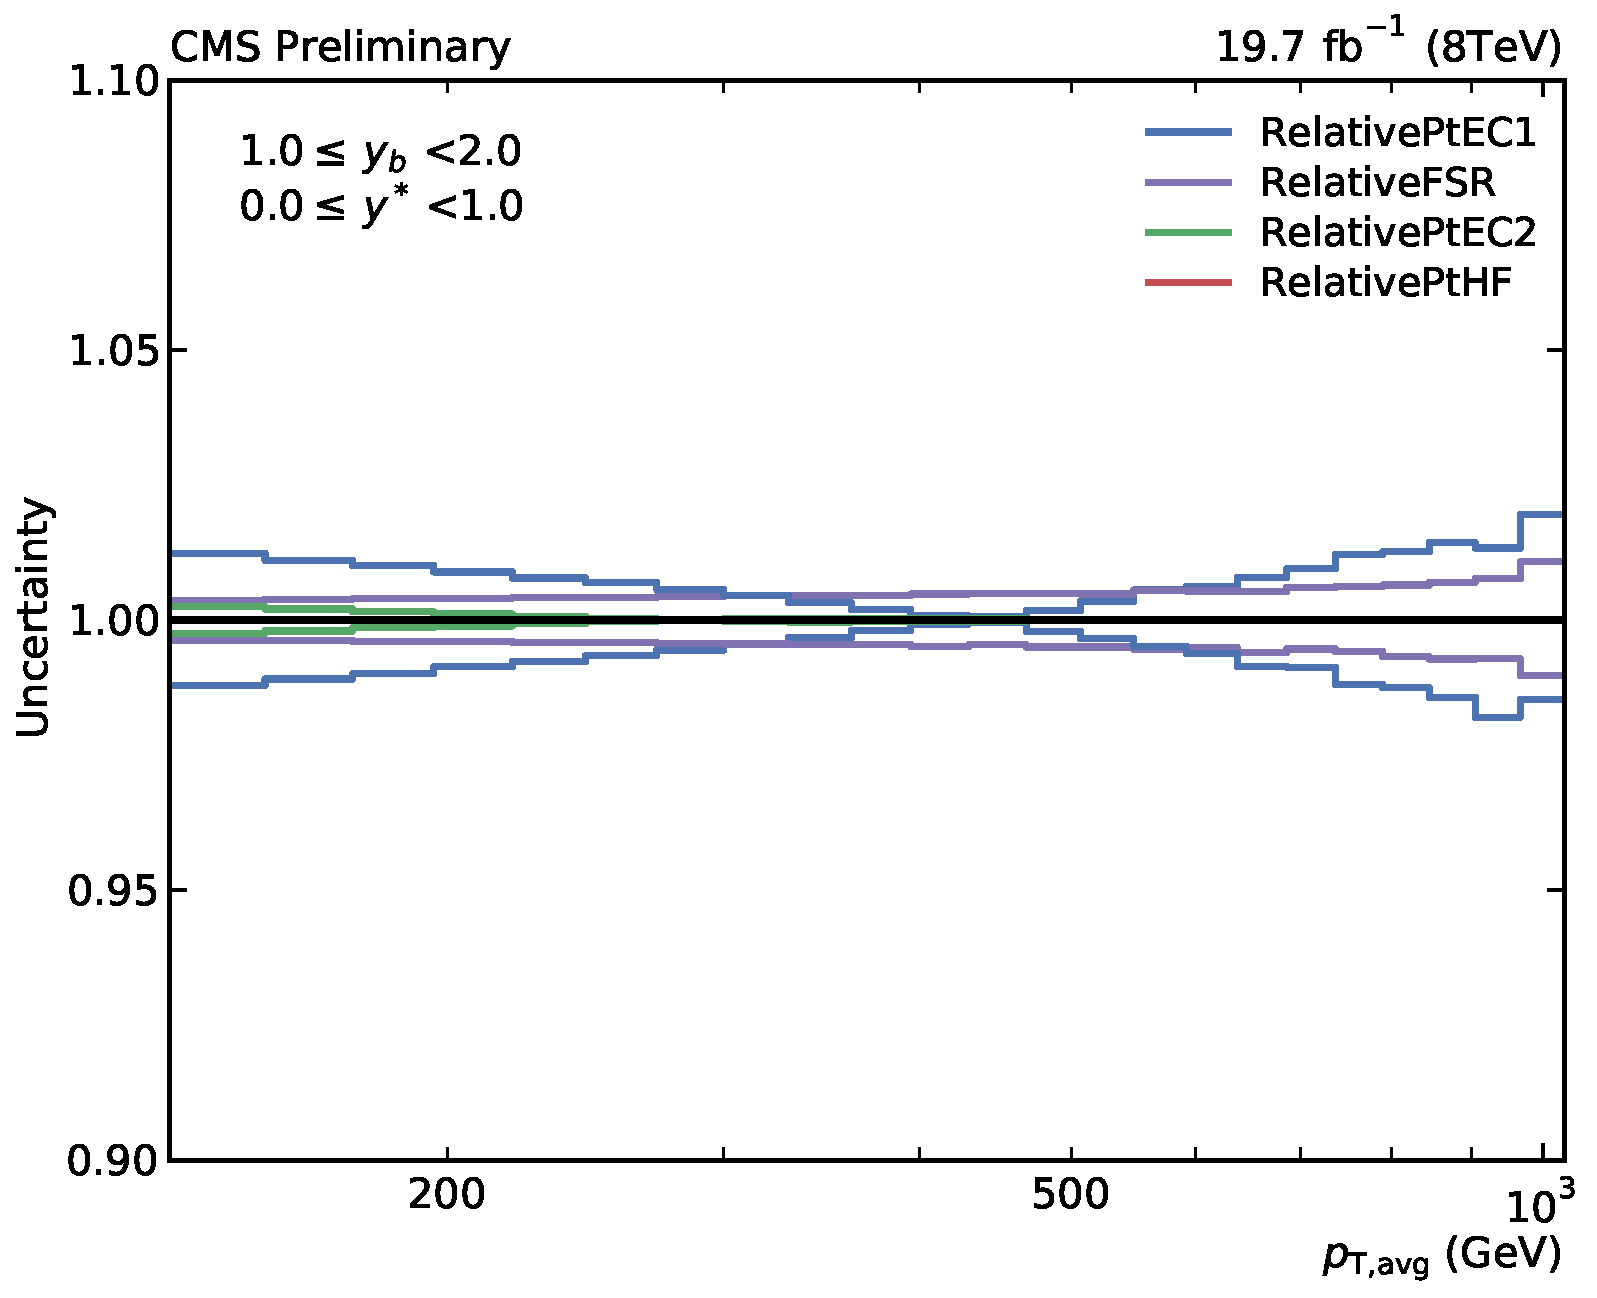
\includegraphics[width=0.45\textwidth]{figures/measurement/jec_relunc_3_yb1ys0.pdf}
    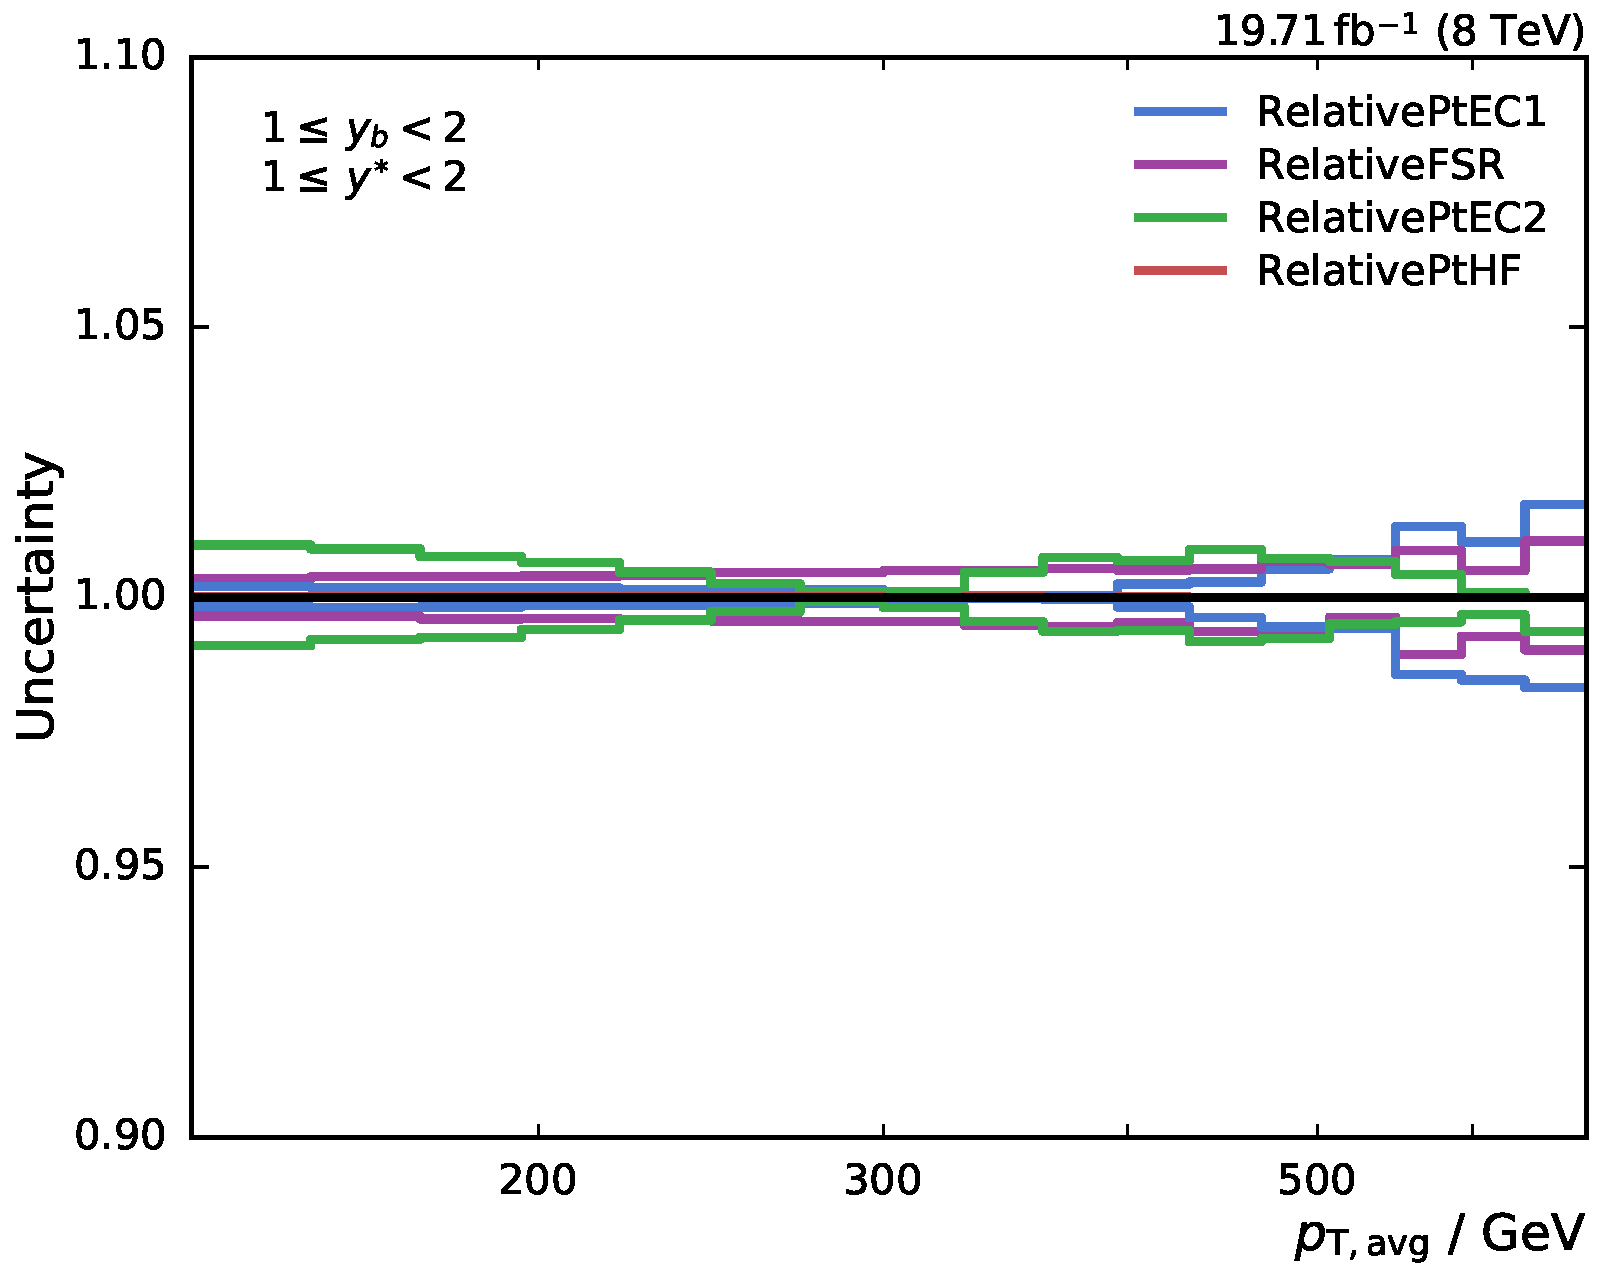
\includegraphics[width=0.45\textwidth]{figures/measurement/jec_relunc_3_yb1ys1.pdf}\hfill
    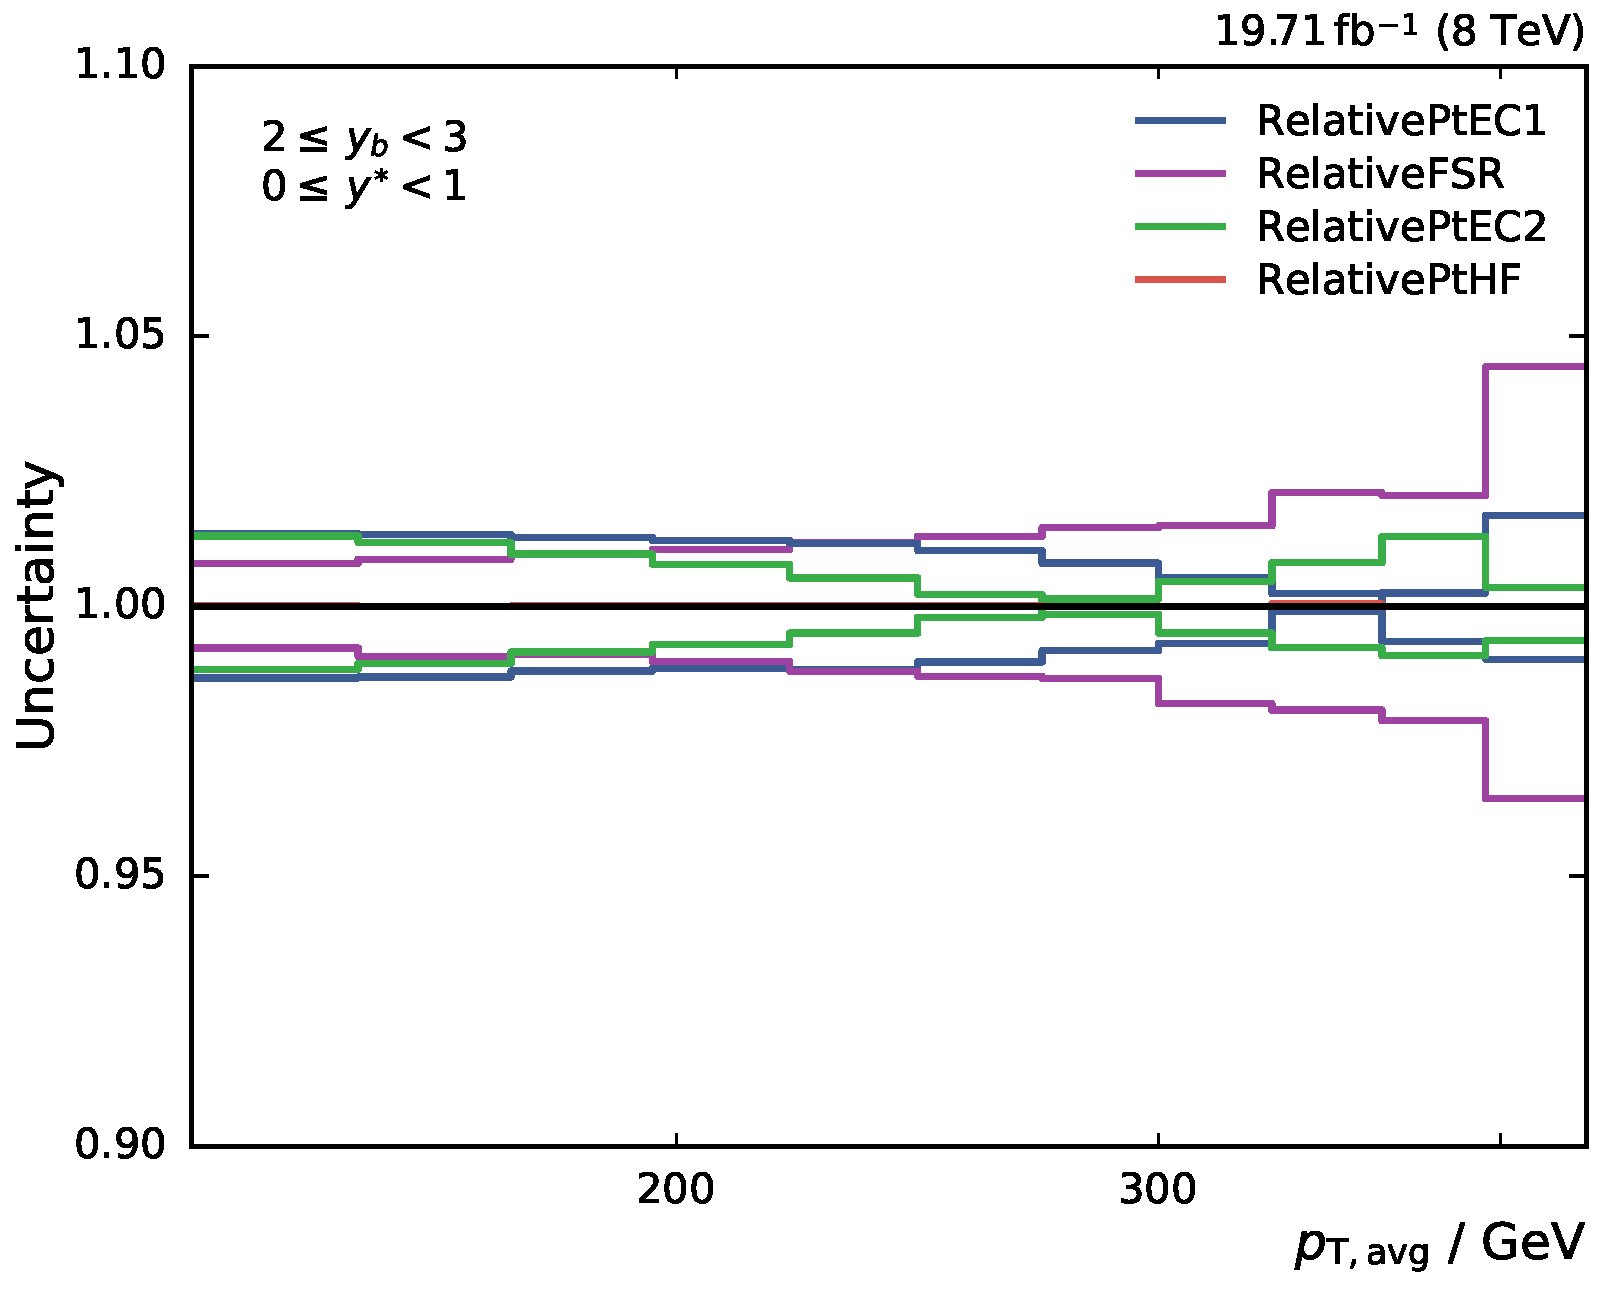
\includegraphics[width=0.45\textwidth]{figures/measurement/jec_relunc_3_yb2ys0.pdf}
    \caption{Splitup of the uncertainties due to jet energy corrections.}
    \label{fig:jec_relunc_3}
\end{figure}

\begin{figure}[htbp]
    \centering
    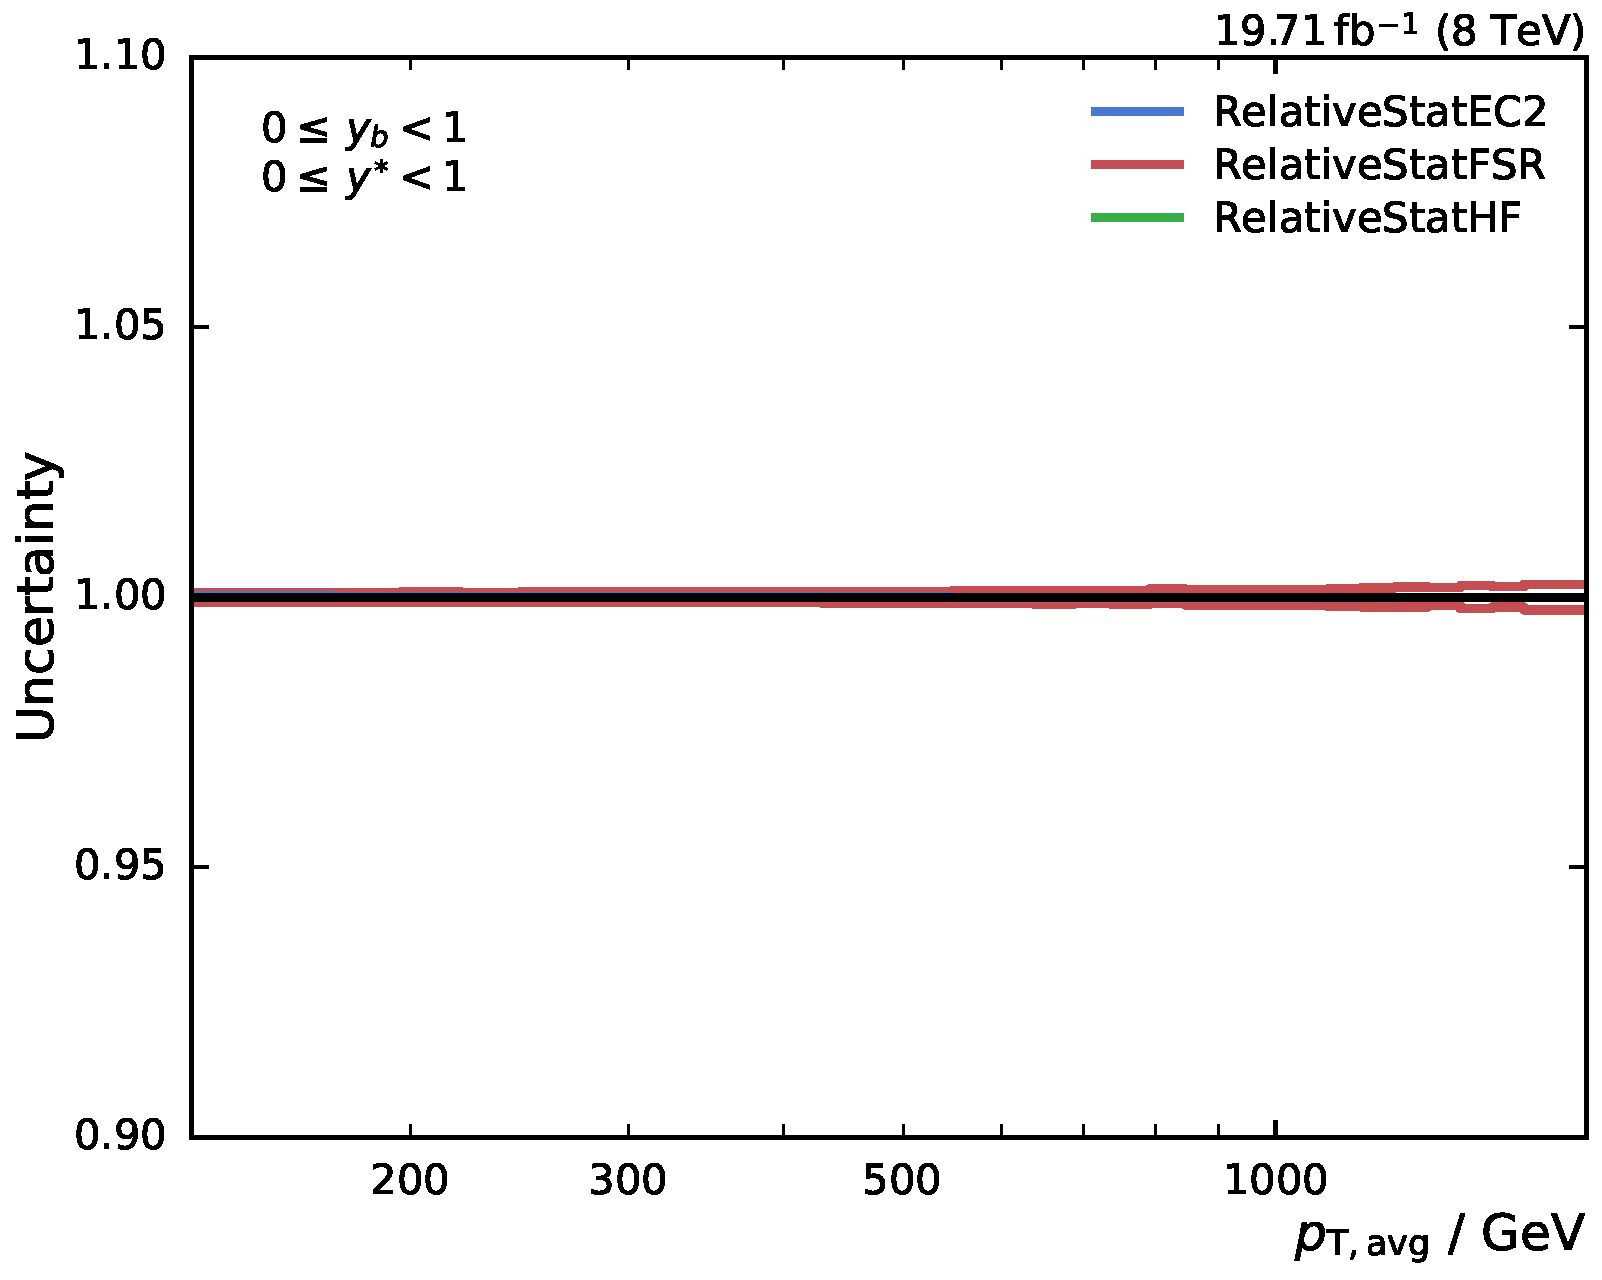
\includegraphics[width=0.45\textwidth]{figures/measurement/jec_relunc_4_yb0ys0.pdf}\hfill
    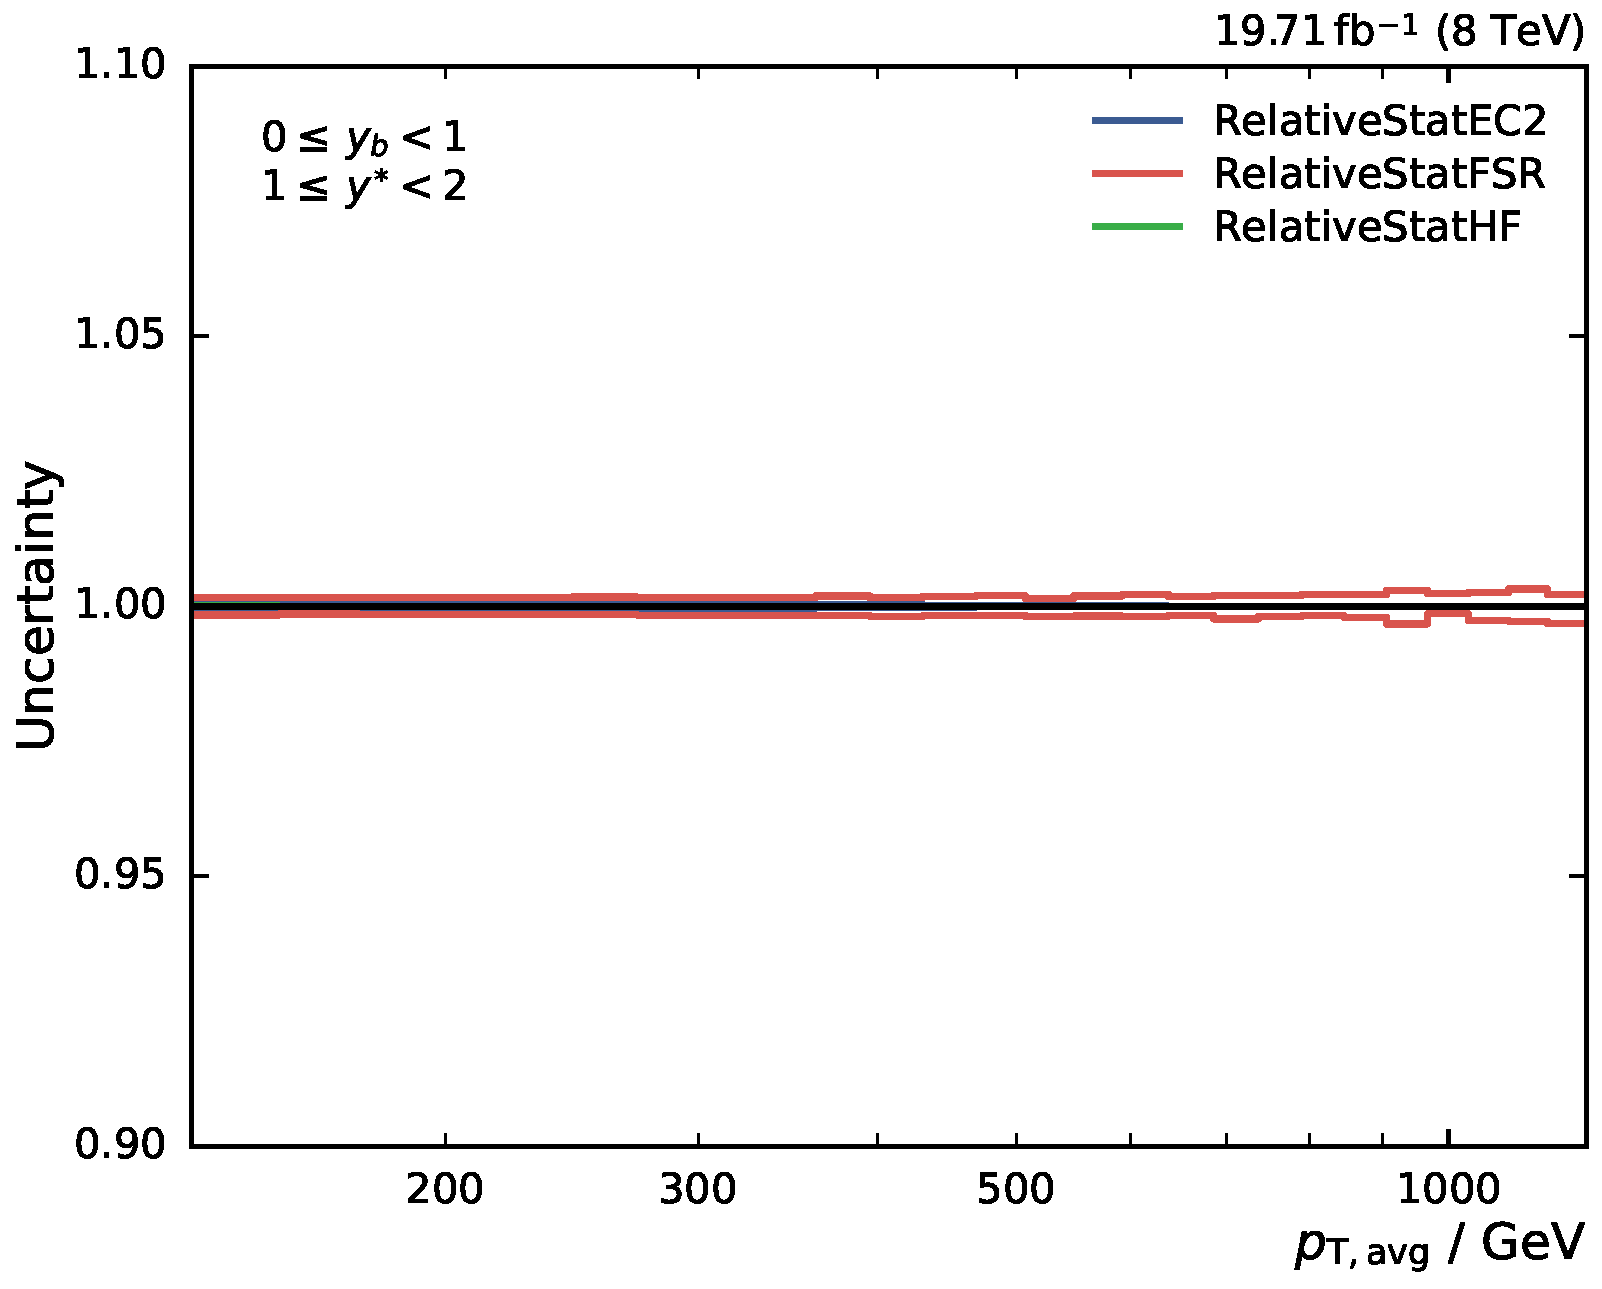
\includegraphics[width=0.45\textwidth]{figures/measurement/jec_relunc_4_yb0ys1.pdf}
    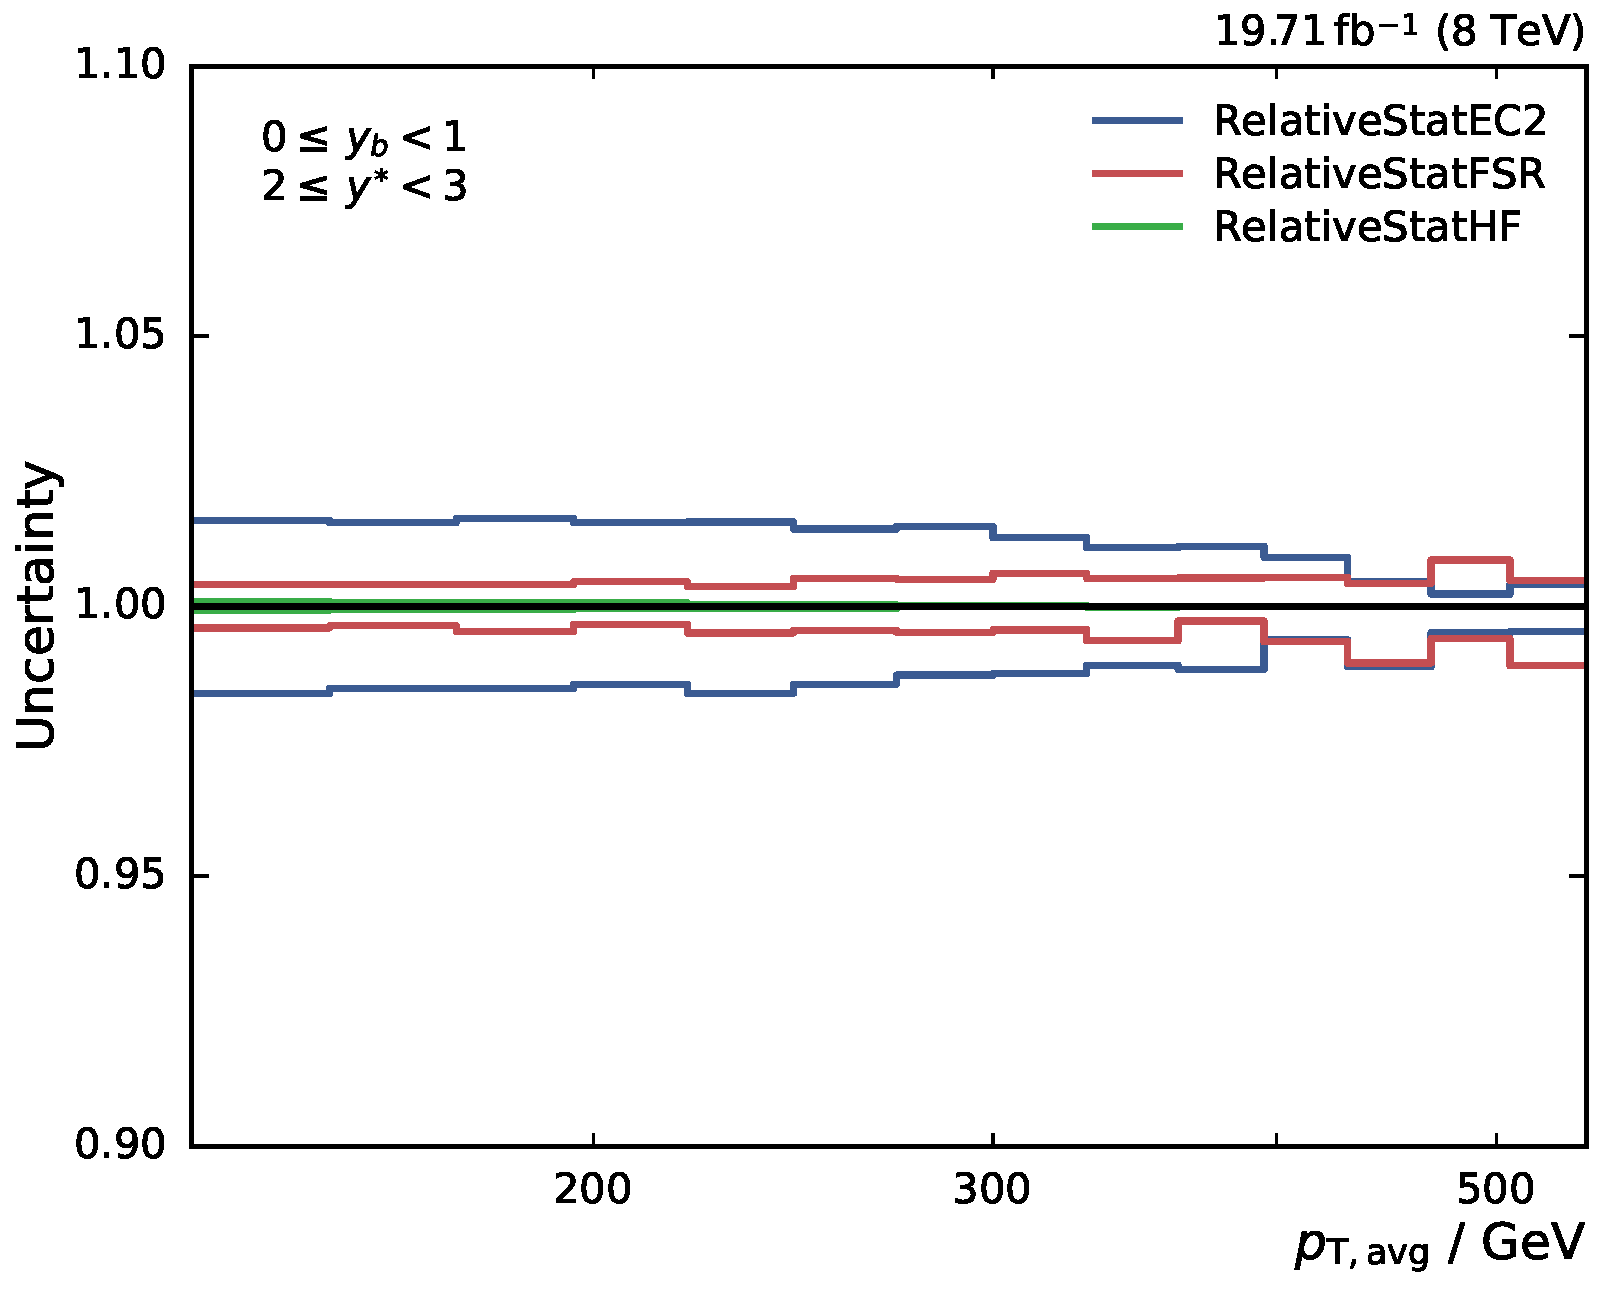
\includegraphics[width=0.45\textwidth]{figures/measurement/jec_relunc_4_yb0ys2.pdf}\hfill
    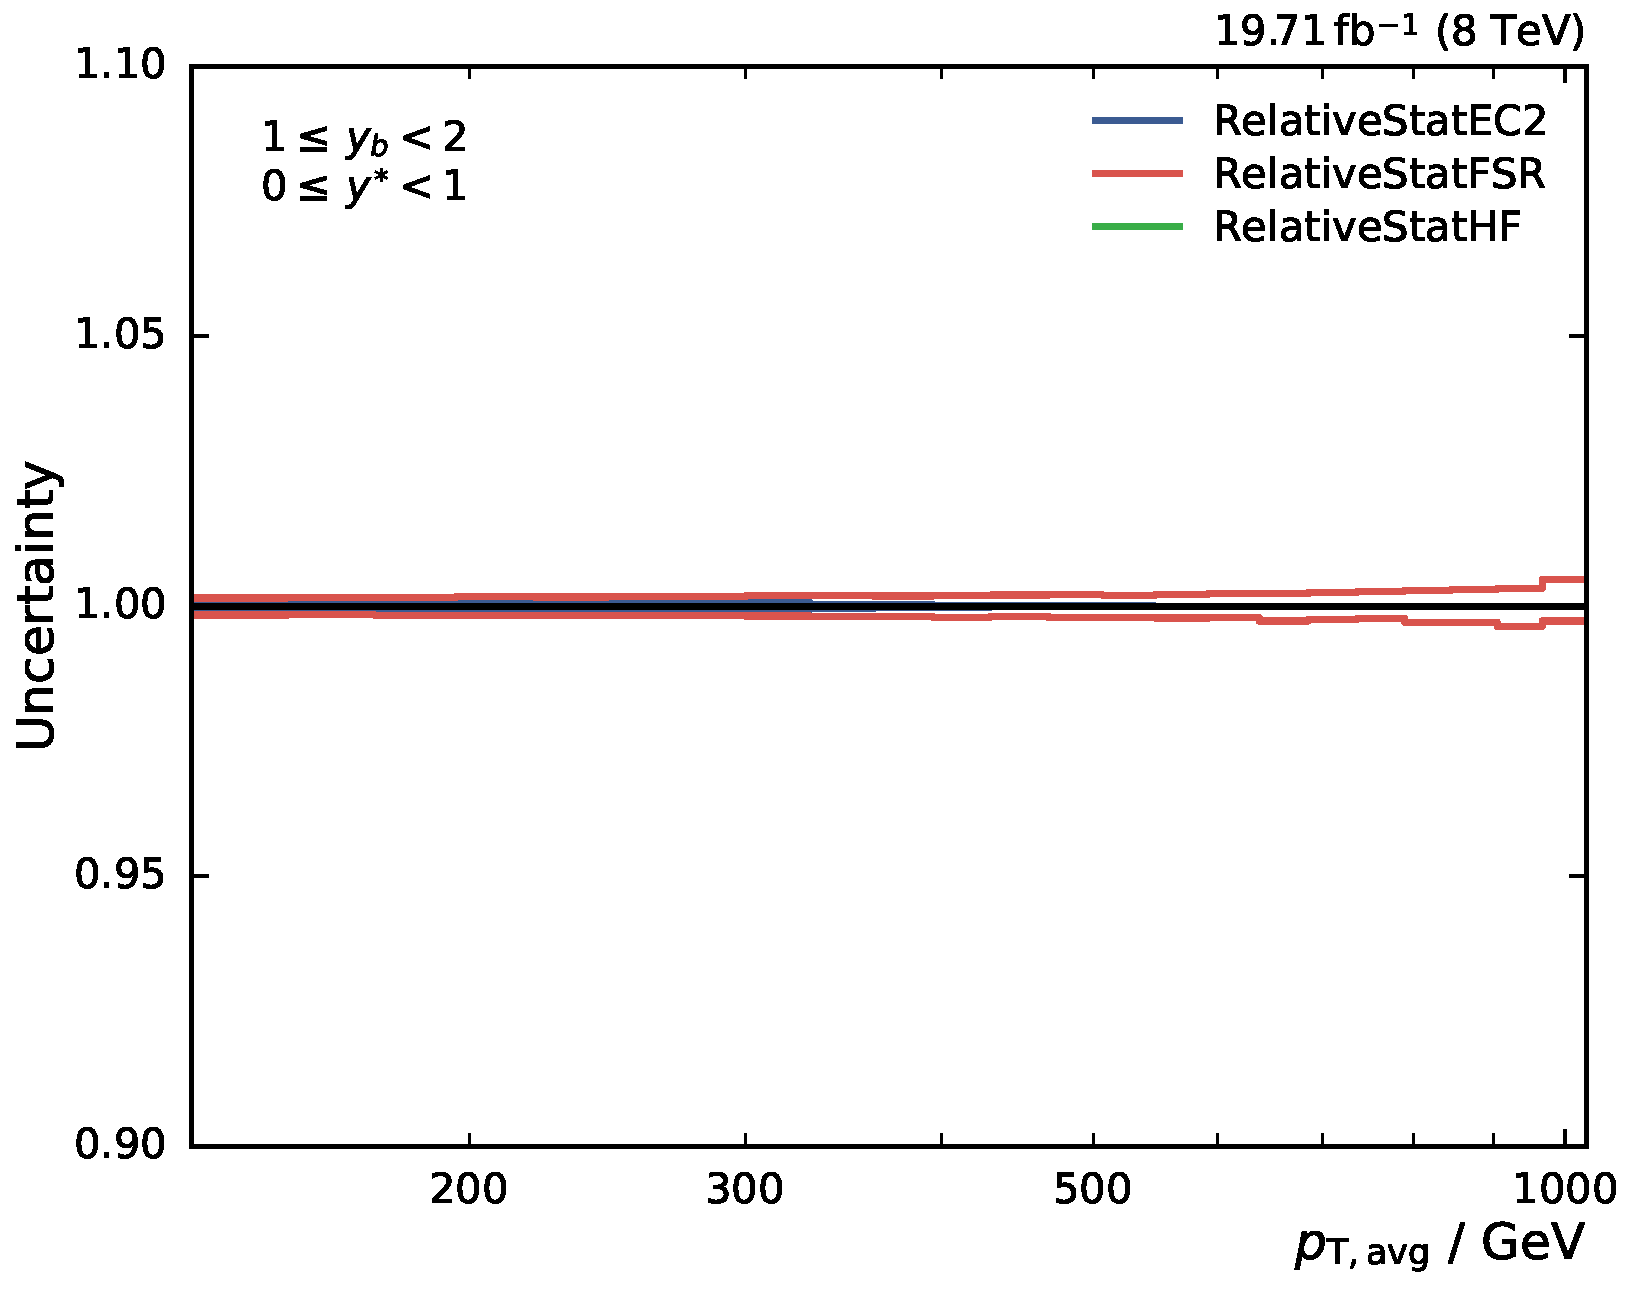
\includegraphics[width=0.45\textwidth]{figures/measurement/jec_relunc_4_yb1ys0.pdf}
    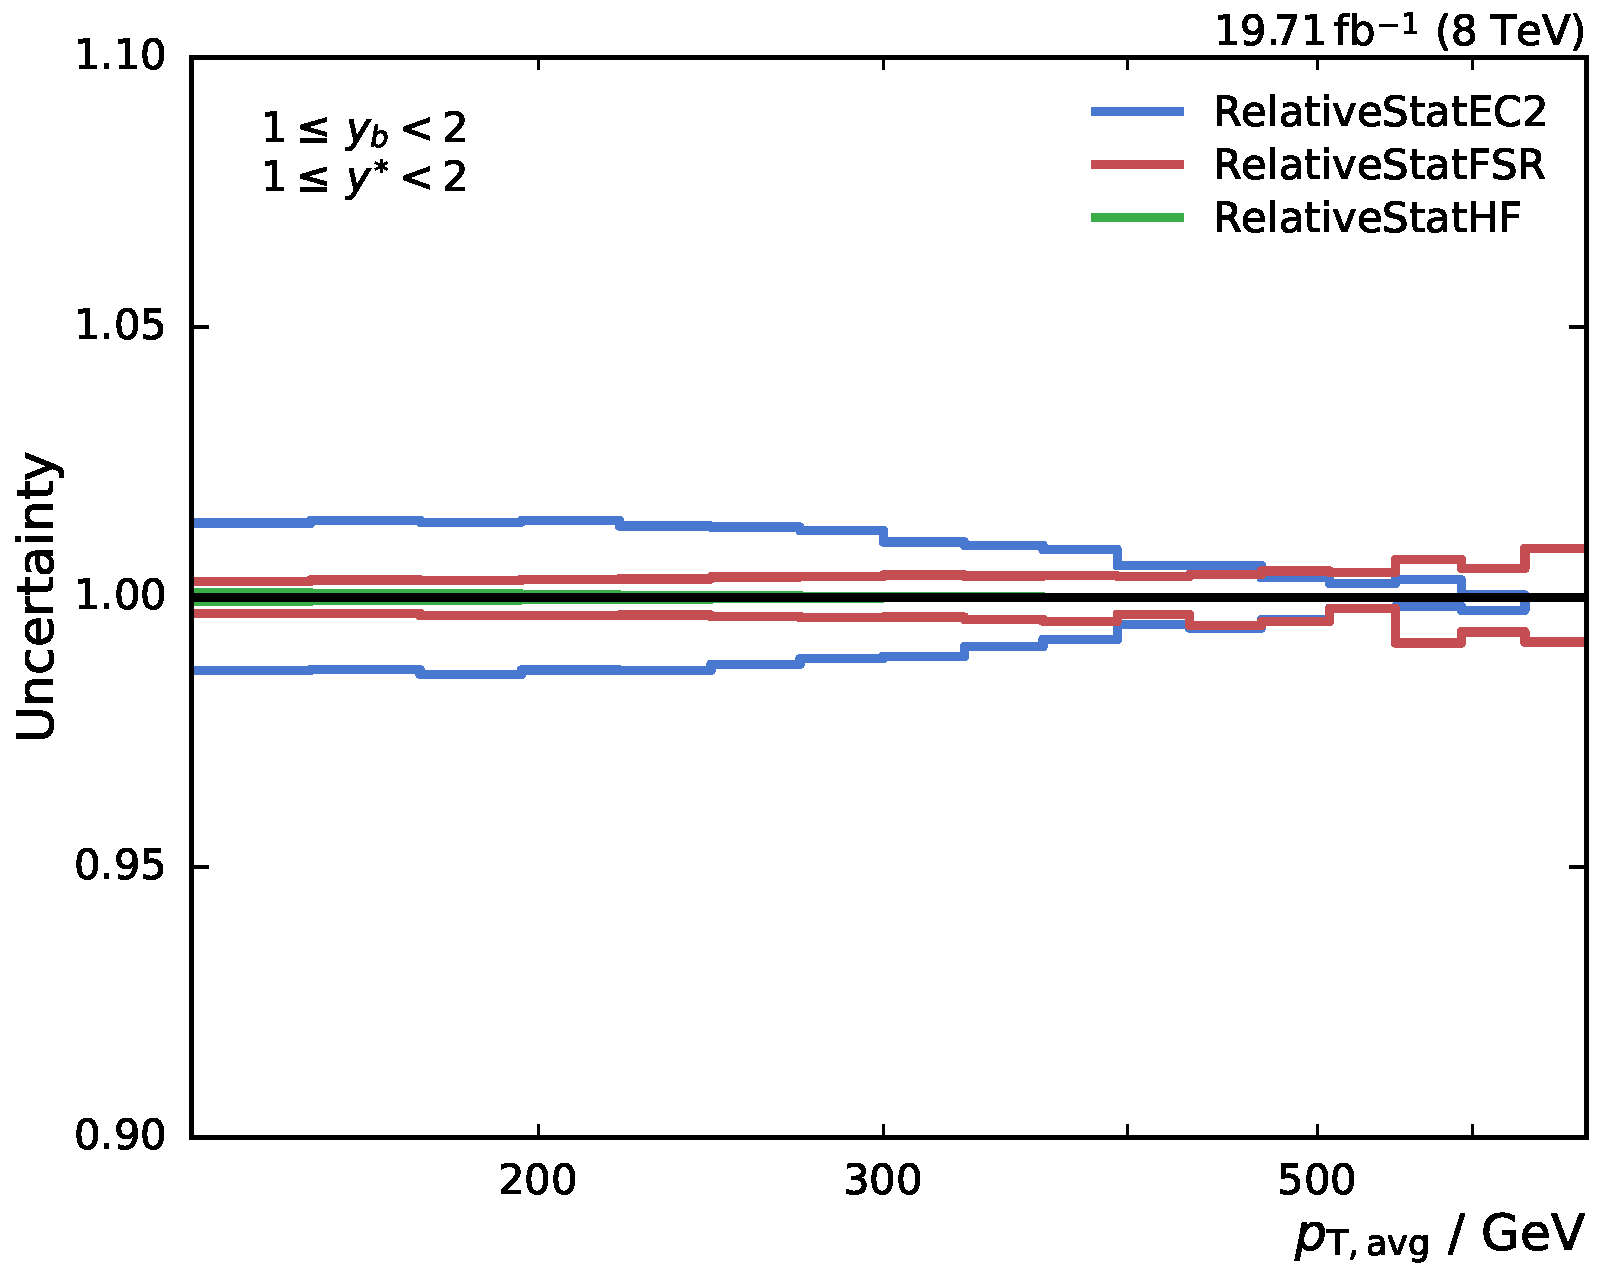
\includegraphics[width=0.45\textwidth]{figures/measurement/jec_relunc_4_yb1ys1.pdf}\hfill
    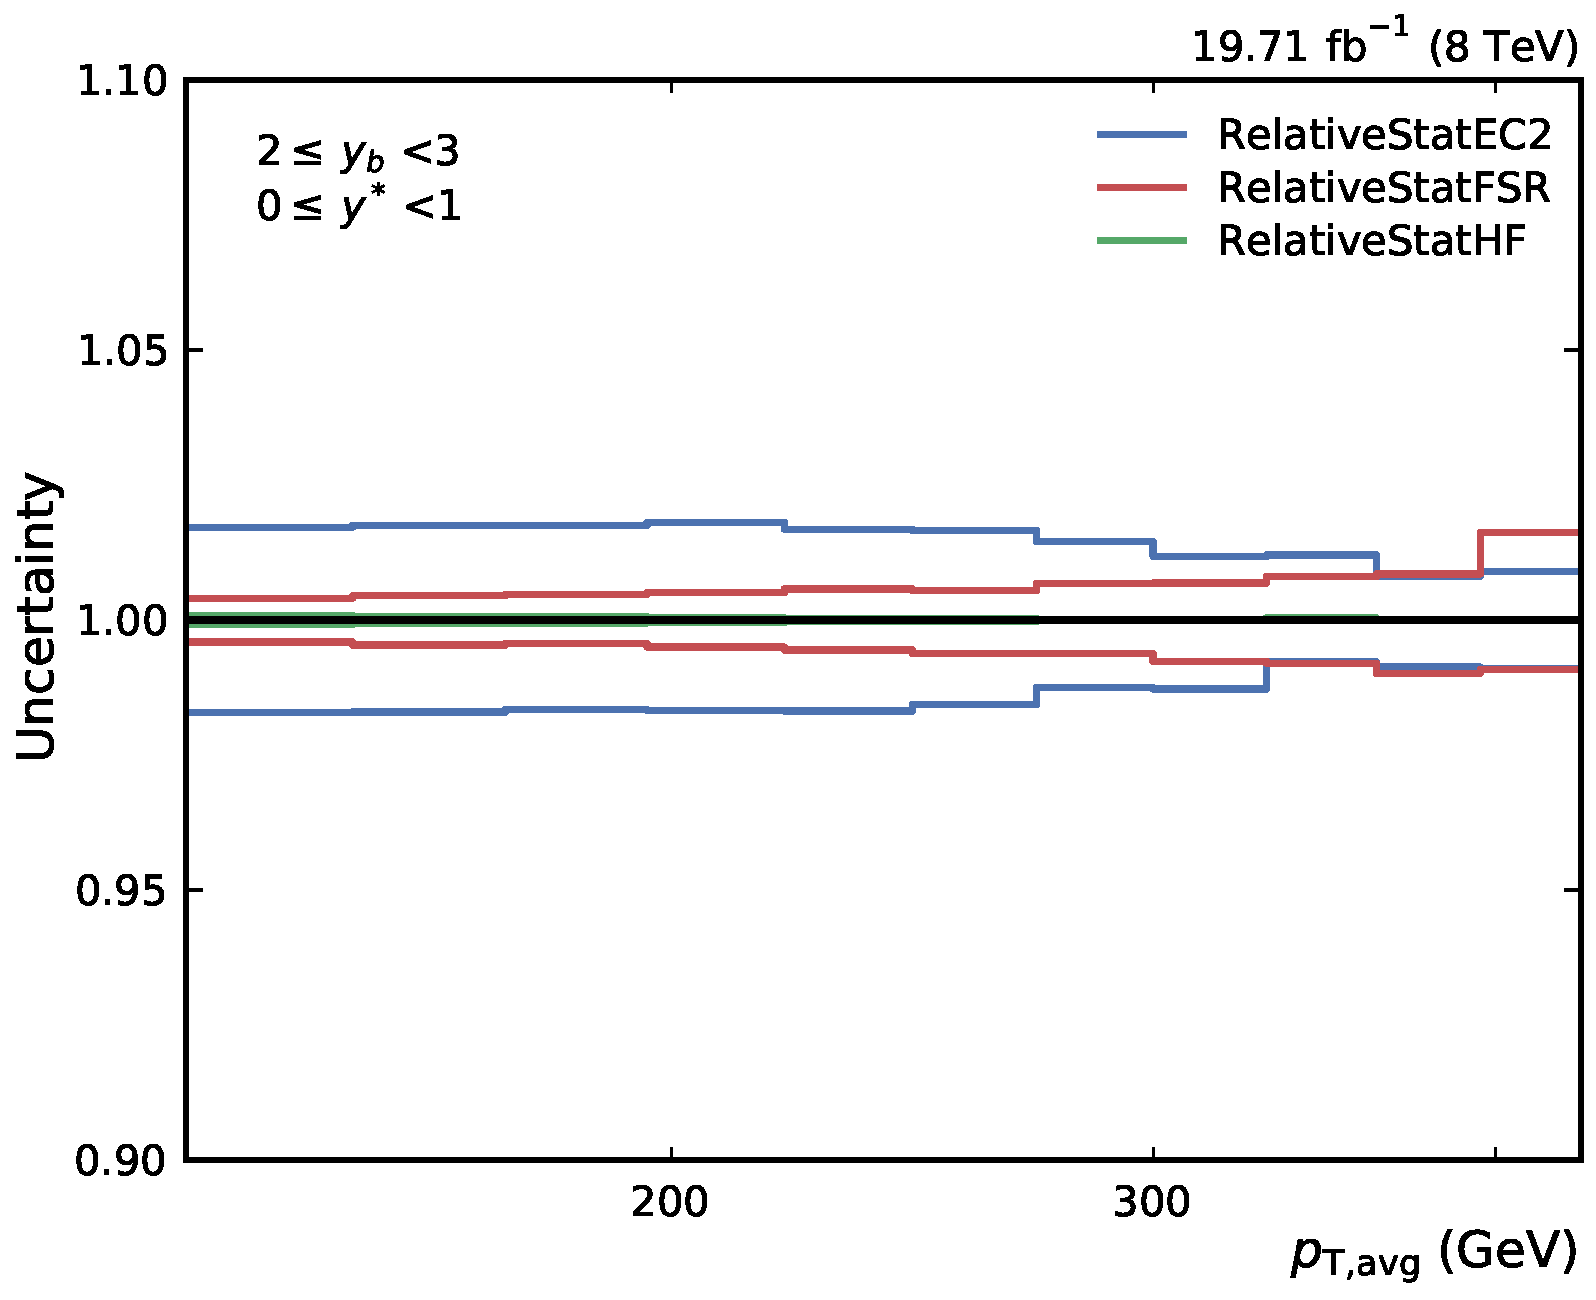
\includegraphics[width=0.45\textwidth]{figures/measurement/jec_relunc_4_yb2ys0.pdf}
    \caption{Splitup of the uncertainties due to jet energy corrections.}
    \label{fig:jec_relunc_4}
\end{figure}

\begin{figure}[htbp]
    \centering
    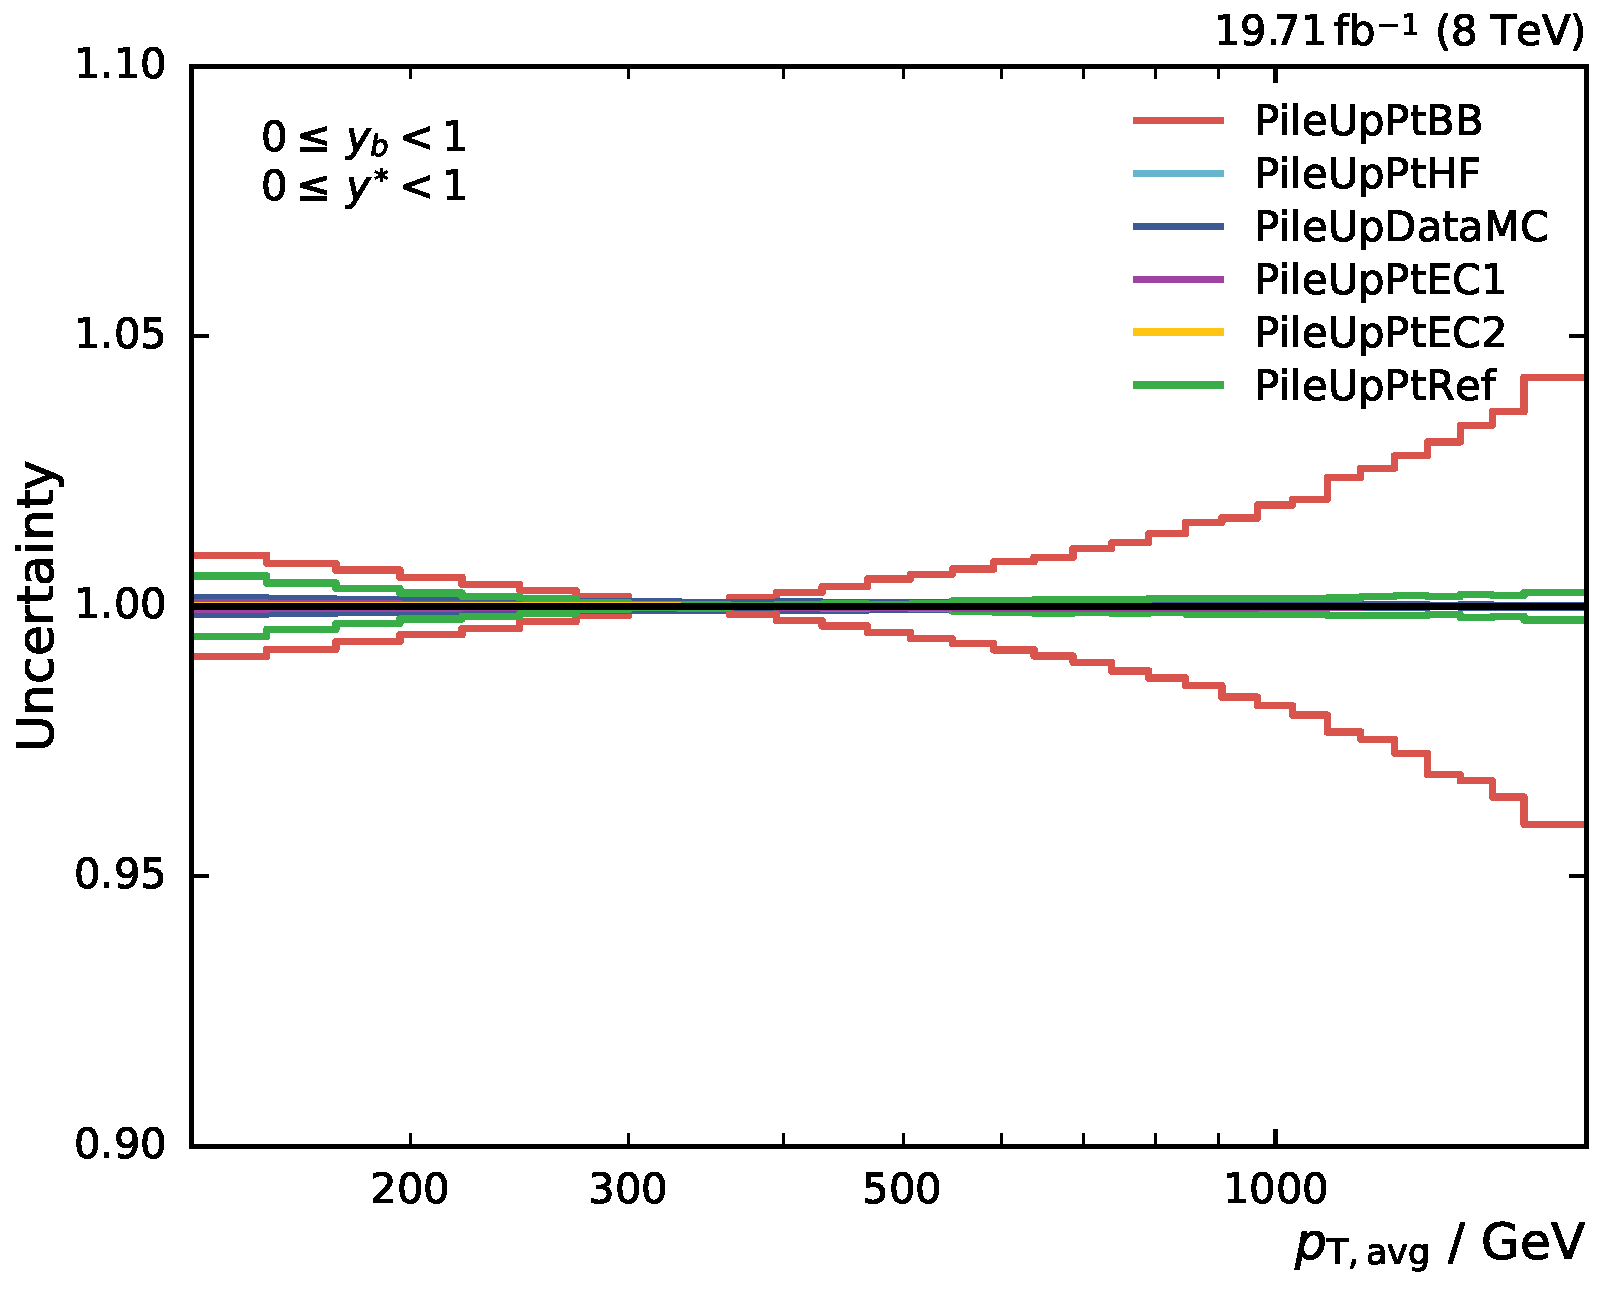
\includegraphics[width=0.45\textwidth]{figures/measurement/jec_relunc_5_yb0ys0.pdf}\hfill
    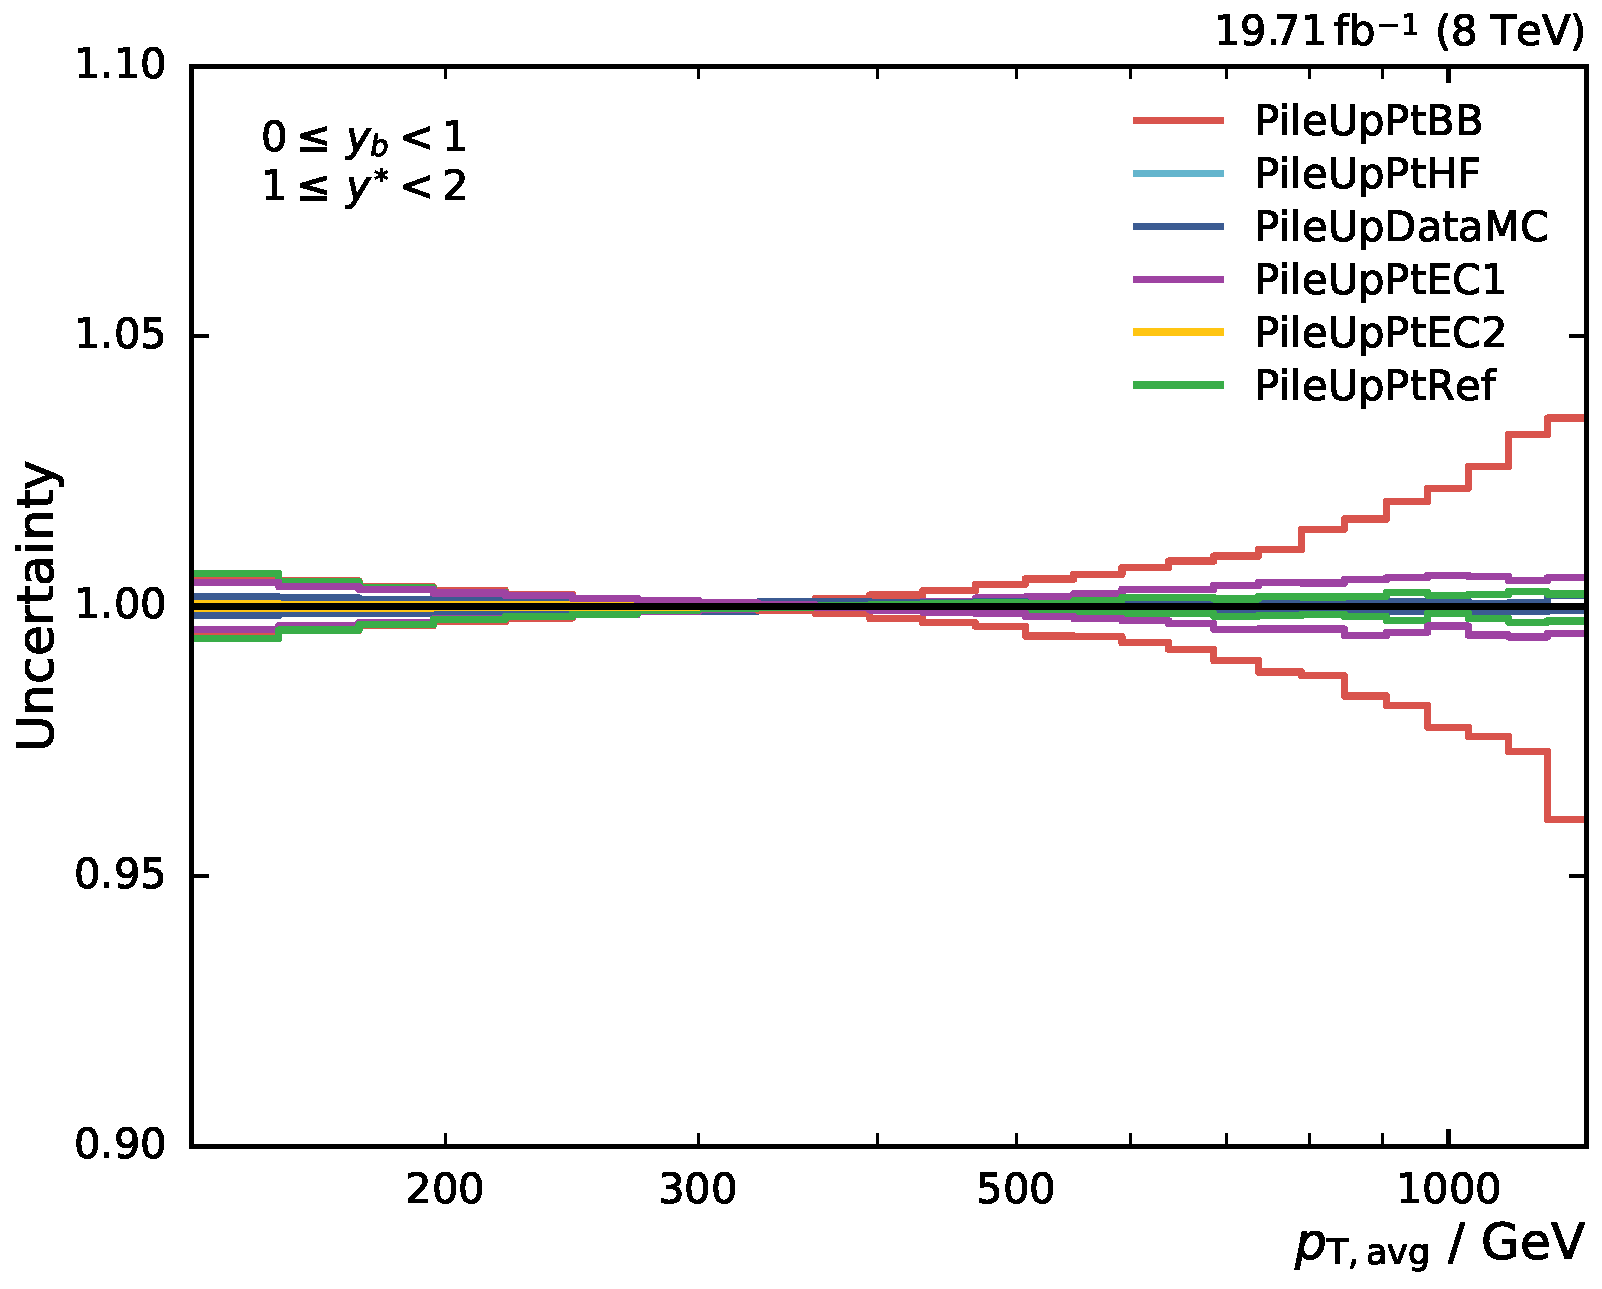
\includegraphics[width=0.45\textwidth]{figures/measurement/jec_relunc_5_yb0ys1.pdf}
    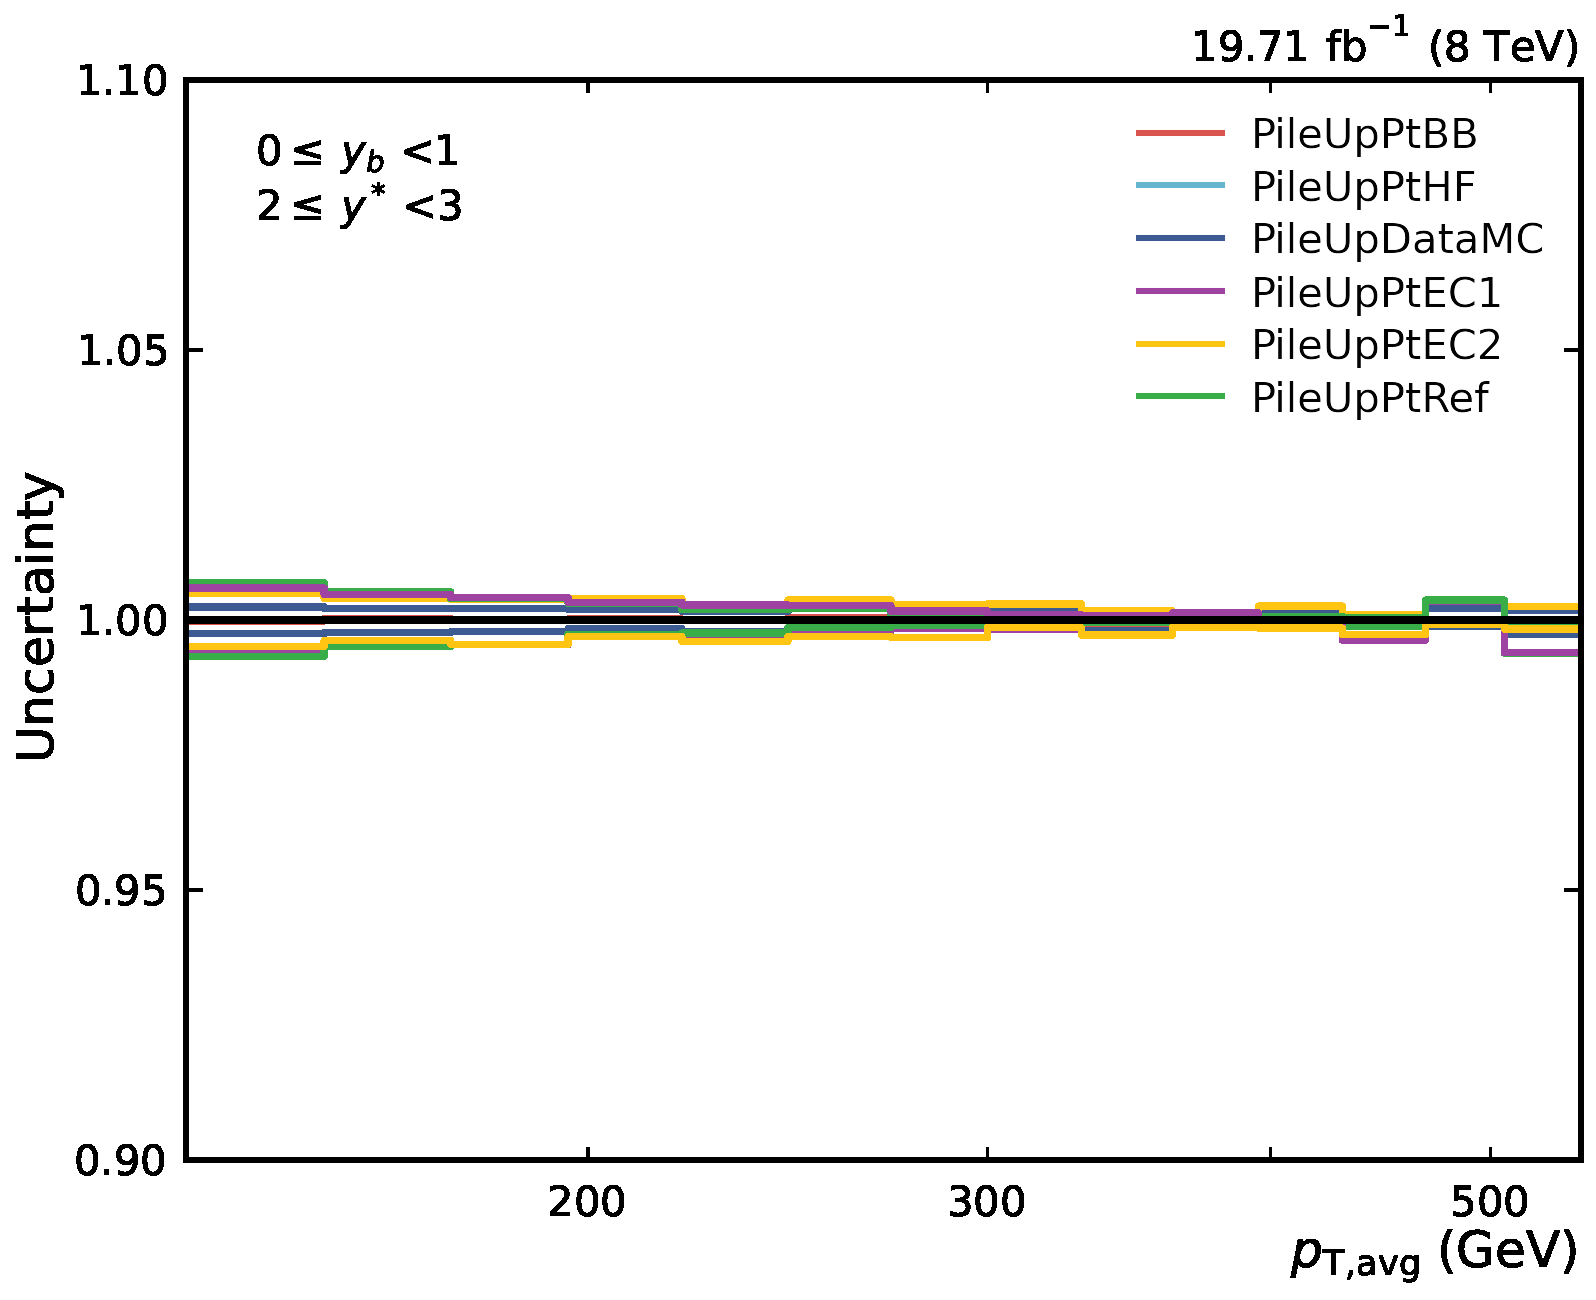
\includegraphics[width=0.45\textwidth]{figures/measurement/jec_relunc_5_yb0ys2.pdf}\hfill
    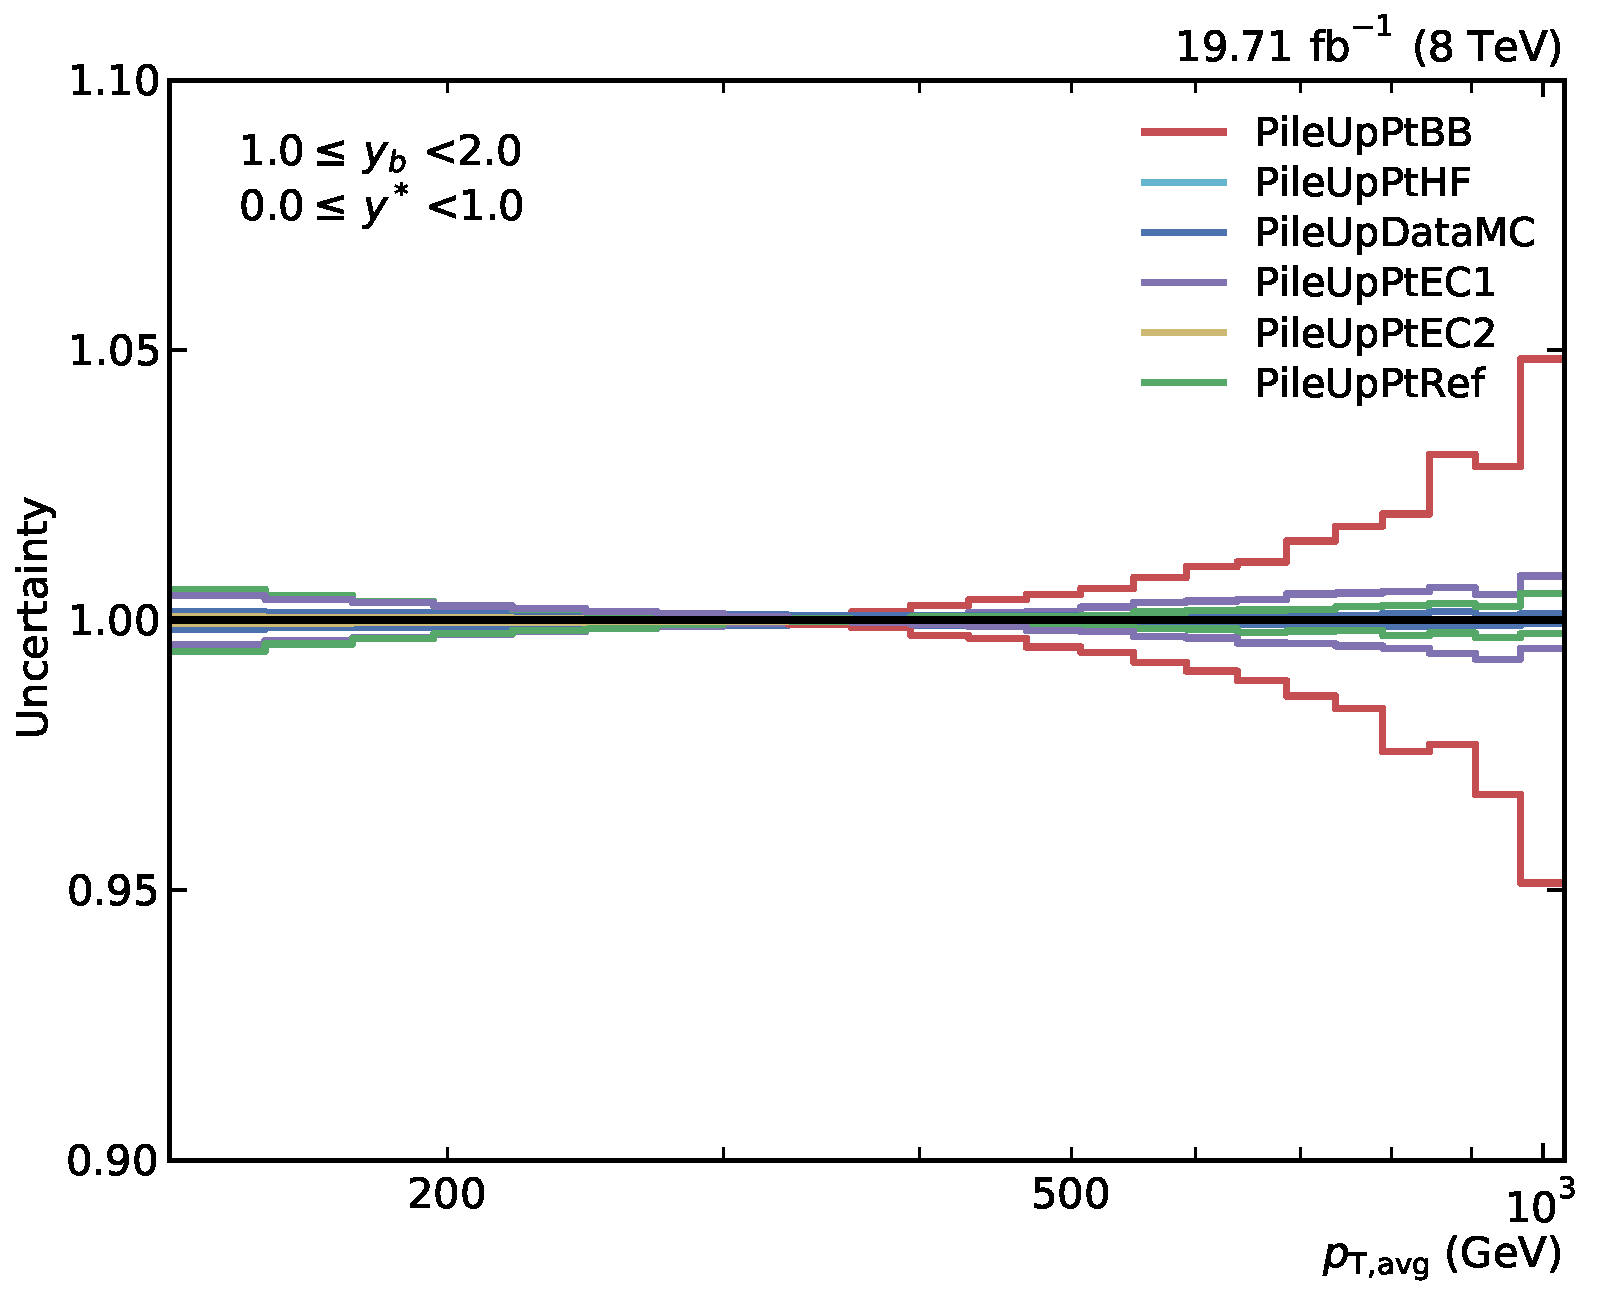
\includegraphics[width=0.45\textwidth]{figures/measurement/jec_relunc_5_yb1ys0.pdf}
    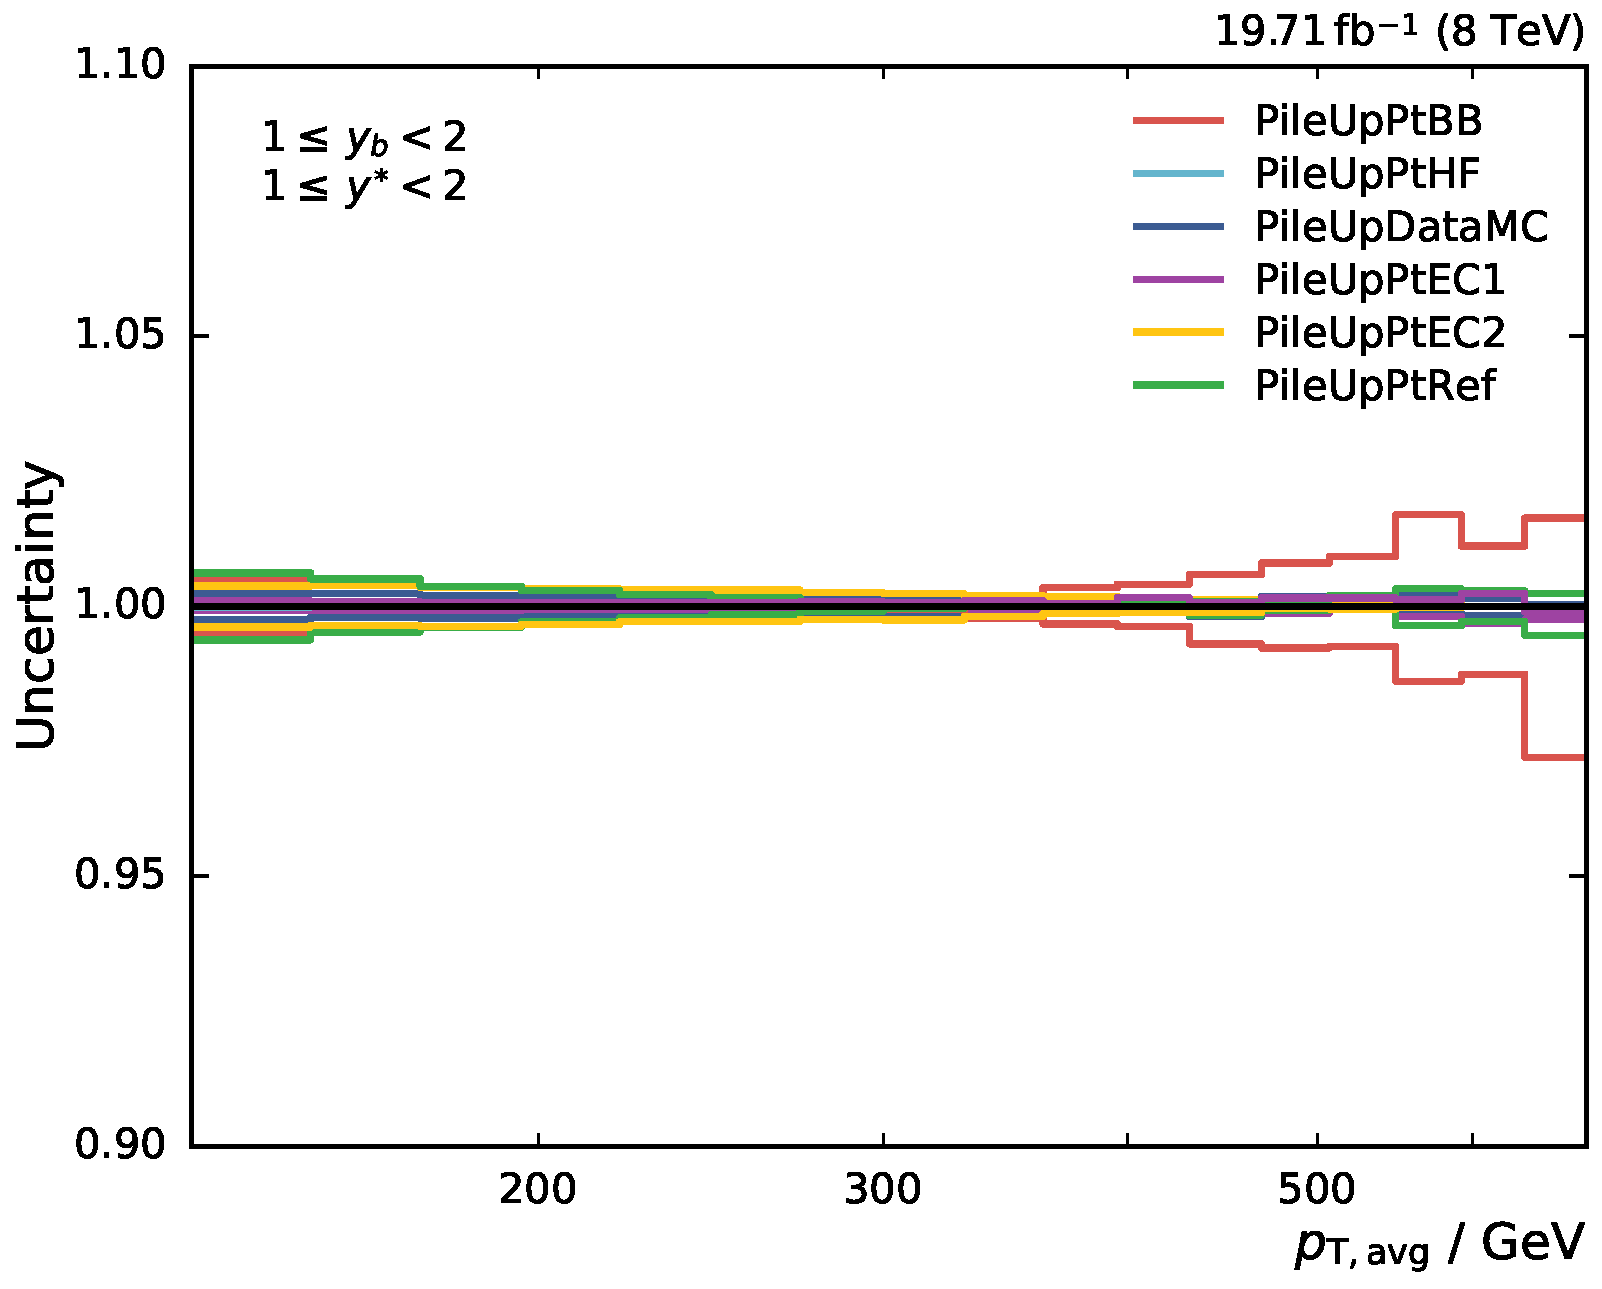
\includegraphics[width=0.45\textwidth]{figures/measurement/jec_relunc_5_yb1ys1.pdf}\hfill
    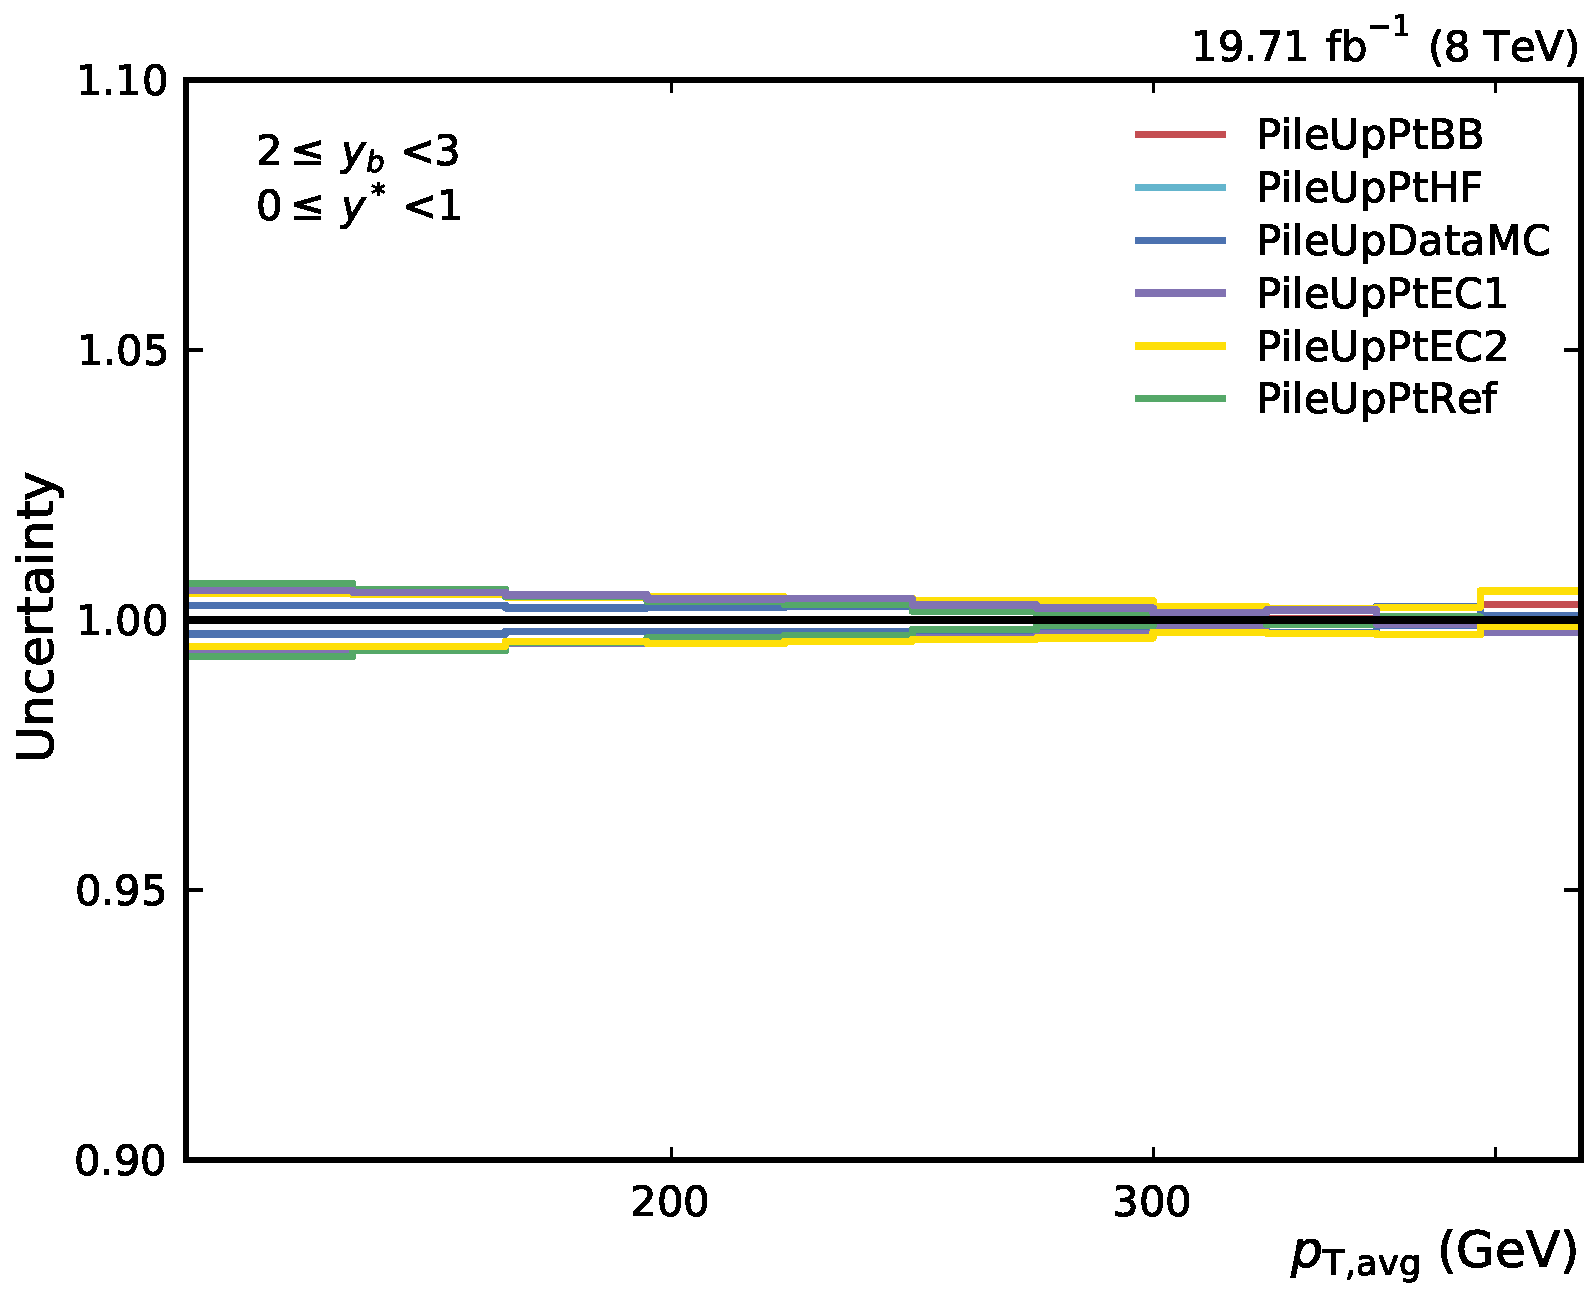
\includegraphics[width=0.45\textwidth]{figures/measurement/jec_relunc_5_yb2ys0.pdf}
    \caption{Splitup of the uncertainties due to jet energy corrections.}
    \label{fig:jec_relunc_5}
\end{figure}

